%!TEX root = ../ThesisRomainbrault.tex

\chapter{Operator-valued functions and integration}
\label{ch:operator-valued_functions_and_integration}

\chapter{Proofs of theorems}
\label{ch:proof_of_theorems}
%!TEX root = ../../ThesisRomainbrault.tex

\section{Proof of the error bound with high probability of the ORFF
estimator}
\label{subsec:concentration_proof}
We recall the notations $\delta=x\groupop z^{-1}$, for all $x$,
$z\in\mathcal{X}$,
$\tilde{K} (x,z) = {\tildePhi{\omega} (x)}^\adjoint \tildePhi{\omega} (z)$,
$\tilde{K}^j (x,z) = {\Phi_x (\omega_j)}^\adjoint \Phi_z (\omega_j)$, where
$\omega_j\sim\probability_{\dual{\Haar,\rho}}$ and $K_e (\delta)=K(x,z)$ and
$\tilde{K}_e(\delta)=\tilde{K}(x,z)$. For the sake of readabilty, we use
throughout the proof the quantities
\begin{dgroup*}
    \begin{dmath*}
        F (\delta)\colonequals\tilde{K} (x,z) - K (x,z)
    \end{dmath*}
    \begin{dmath*}
        F^j (\delta)\colonequals\frac{1}{D} \left(\tilde{K}^j (x,z) - K
        (x,z)\right) 
    \end{dmath*}
\end{dgroup*}
We also view $\mathcal{X}$ as a metric space endowed with the distance
$d_{\mathcal{X}}:\mathcal{X}\times\mathcal{X}\to\mathbb{R}_+$. Compared to the
scalar case, the proof follows the same scheme as the one described in
\citep{Rahimi2007, sutherland2015}, but we consider an operator norm as measure
of the error and therefore concentration inequality dealing with these operator
norm.  The main feature of \cref{pr:bound_approx_unbounded} is that it covers
the case of bounded \acs{ORFF} as well as unbounded \acs{ORFF}. In the case of
bounded \acs{ORFF}, a Bernstein inequality for matrix concentration such that
the one proved in \citet[Corollary 5.2]{Mackey2014} or the formulation of
\citet{Tropp} recalled in \citet{koltchinskii2013remark}~is suitable. However
some kernels like the curl and the divergence-free kernels do not have obvious
bounded $\norm{F^j}_{\mathcal{Y},\mathcal{Y}}$ but exhibit $F^j$ with
subexponential tails. Therefore, we use an operator Bernstein concentration
inequality adapted for random matrices with subexponential norms.
\subsection{Epsilon-net}
\label{subsec:epsilon-net}
Let $\mathcal{C}\subseteq\mathcal{X}$ be a compact subset of $\mathcal{X}$. Let
$\mathcal{D}_{\mathcal{C}} = \Set{x\groupop z^{-1} | x, z\in\mathcal{C} }$ with
diameter at most $2\abs{\mathcal{C}}$ where $\abs{\mathcal{C}}$ is the diameter
of $\mathcal{C}$. Since $\mathcal{C}$ is supposed compact, so is
$\mathcal{D}_{\mathcal{C}}$. Since $\mathcal{D}_{\mathcal{C}}$ is also a metric
space it is well known that a compact metric space is totally bounded. Thus it
is possible to find a finite $\epsilon$-net covering
$\mathcal{D}_{\mathcal{C}}$. We call $T=\mathcal{N}(\mathcal{D}_{\mathcal{C}},
r)$ the number of closed balls of radius $r$ required to cover
$\mathcal{D}_{\mathcal{C}}$. For instance if $\mathcal{D}_{\mathcal{C}}$ is a
subspace finite dimensional Banach space with diameter at most
$2\abs{\mathcal{C}}$ it is possible to cover the space with at most
$T={(4\abs{\mathcal{C}}/r)}^d$ balls of radius $r$
(see \citet[proposition 5]{cucker2001mathematical}).
\paragraph{}
Let us call $\delta_i,i=1,\ldots,T$ the center of the $i$-th ball, also called
anchor of the $\epsilon$-net. Denote $L_{F}$ the Lipschitz constant of $F$. Let
$\norm{\cdot}_{\mathcal{Y},\mathcal{Y}}$ be the operator norm on
$\mathcal{L}(\mathcal{Y})$ (largest eigenvalue). We introduce the following
technical lemma.
\begin{lemma}\label{lm:error_decomposition}
    $\forall \delta \in \mathcal{D}_{\mathcal{C}}$, if
    \begin{dmath}
        L_{F}\le\frac{\epsilon}{2r}\label{condition1}
    \end{dmath}
    and
    \begin{dmath}
        \norm{F (\delta_i)}_{\mathcal{Y},\mathcal{Y}}
        \le\frac{\epsilon}{2}\condition{for all
        $i\in\mathbb{N}^*_T$}\label{condition2}
    \end{dmath}
    then $\norm{F(\delta)}_{\mathcal{Y},\mathcal{Y}} \leq \epsilon$.
\end{lemma}
\begin{proof}
    \begin{dmath*}
        \norm{F (\delta)}_{\mathcal{Y},\mathcal{Y}} = \norm{F (\delta) -
        F(\delta_i) + F(\delta_i)}_{\mathcal{Y},\mathcal{Y} }\le
        \norm{F(\delta) - F(\delta_i)}_{\mathcal{Y},\mathcal{Y}} +
        \norm{F(\delta_i)}_{\mathcal{Y},\mathcal{Y}}
    \end{dmath*}
    for all $0<i<T$. Using the Lipschitz continuity of $F$ we have 
    \begin{dmath*}
        \norm{F(\delta) - F(\delta_i)}_{\mathcal{Y},\mathcal{Y}} \le
        d_{\mathcal{X}}(\delta,\delta_i) L_{F} \hiderel{\le} rL_{F}
    \end{dmath*}
    hence
    \begin{dmath*}
        \norm{F(\delta)}_{\mathcal{Y},\mathcal{Y}} \le rL_{F} +
        \norm{F(\delta_i)}_{\mathcal{Y},\mathcal{Y}} \hiderel{=}
        \frac{r\epsilon}{2 r} + \frac{\epsilon}{2} \hiderel{=} \epsilon.
    \end{dmath*}
\end{proof}
To apply the lemma, we must bound the Lipschitz constant of the operator-valued
function $F$ (\cref{condition1}) and
$\norm{F(\delta_i)}_{\mathcal{Y},\mathcal{Y}}$, for all $i=1, \ldots, T$ as
well (\cref{condition2}).
\subsection{Bounding the Lipschitz constant}
This proof is a slight generalization of \citet{minh2016operator} to arbitrary
metric spaces. It differ from our first approach \citep{brault2016random},
based on the proof of \citet{sutherland2015} which was only valid for a finite
dimensional input space $\mathcal{X}$ and imposed a twice differentiability
condition on the considered kernel.
\begin{lemma}
    \label{lm:LipschitzK}
    Let $H_\omega \in \mathbb{R}_+$ be the Lipschitz constant of
    $h_\omega(\cdot)$ and assume that
    \begin{dmath*}
        \int_{\dual{\mathcal{X}}} H_\omega
        \norm{A(\omega)}_{\mathcal{Y},\mathcal{Y}}d\probability_{\dual{\Haar},
        \rho}(\omega) < \infty.
    \end{dmath*}
    Then the operator-valued function
    $K_e:\mathcal{X}\to\mathcal{L}(\mathcal{Y})$ is Lipschitz with
    \begin{dmath}
        \norm{K_e(x) - K_e(z)}_{\mathcal{Y},\mathcal{Y}}\le
        d_{\mathcal{X}}(x,z) \int_{\dual{\mathcal{X}}} H_\omega
        \norm{A(\omega)}_{\mathcal{Y},\mathcal{Y}}d\probability_{\dual{\Haar},
        \rho}(\omega).
    \end{dmath}
\end{lemma}
\begin{proof}
    We use the fact that the cosine function is Lipschitz with constant $1$ and
    $h_{\omega}$ Lipschitz with constant $H_\omega$. For all $x$,
    $z\in\mathcal{X}$ we have
    \begin{dmath*}
        \norm{\tilde{K}_e(x) - K_e(z)}_{\mathcal{Y},\mathcal{Y}}
        = \norm{\int_{\dual{\mathcal{X}}} \left(\cos h_\omega(x) - \cos
        h_\omega(z)\right)A(\omega)d\probability_{\dual{\Haar},\rho}
        }_{\mathcal{Y},\mathcal{Y}}
        \le \int_{\dual{\mathcal{X}}} \abs{\cos h_\omega(x) - \cos
        h_\omega(z)}\norm{A(\omega)}_{\mathcal{Y},\mathcal{Y}}
        d\probability_{\dual{\Haar},\rho}
        \le \int_{\dual{\mathcal{X}}} \abs{h_\omega(x) -
        h_\omega(z)}\norm{A(\omega)}_{\mathcal{Y},\mathcal{Y}}
        d\probability_{\dual{\Haar},\rho}
        \le d_{\mathcal{X}}(x, z) \int_{\dual{\mathcal{X}}} H_{\omega}
        \norm{A(\omega)}_{\mathcal{Y},\mathcal{Y}}
        d\probability_{\dual{\Haar},\rho}
    \end{dmath*}
\end{proof}
In the same way, considering $\tilde{K}_e(\delta)=\frac{1}{D}\sum_{j=1}^D\cos
h_{\omega_j}(\delta)A(\omega_j)$, where
$\omega_j\sim\probability_{\dual{\Haar},\rho}$, we can show that $\tilde{K}_e$
is Lipschitz with
\begin{dmath*}
    \norm{\tilde{K}_e(x) - \tilde{K}_e(z)}_{\mathcal{Y},\mathcal{Y}}
    \le d_{\mathcal{X}}(x,z)\frac{1}{D}\sum_{j=1}^DH_{\omega_j}
    \norm{A(\omega_j)}_{\mathcal{Y},\mathcal{Y}}.
\end{dmath*}
Combining the Lipschitz continuity of $\tilde{K}_e$ and $\tilde{K}$
(\cref{lm:LipschitzK}) we obtain
\begin{dmath*}
    \norm{F(x)-F(z)}_{\mathcal{Y},\mathcal{Y}}
    = \norm{\tilde{K}_e(x) - \tilde{K}_e(x) - \tilde{K}_e(z) +
    K_e(z)}_{\mathcal{Y}, \mathcal{Y}} 
    \le \norm{\tilde{K}_e(x) -
    \tilde{K}_e(z)}_{\mathcal{Y}, \mathcal{Y}} + \norm{K_e(x) -
    K_e(z)}_{\mathcal{Y}, \mathcal{Y}}
    \le d_{\mathcal{X}}(x,z)\left(\int_{\dual{\mathcal{X}}} H_\omega
    \norm{A(\omega)}_{\mathcal{Y}, \mathcal{Y}}
    d\probability_{\dual{\Haar},\rho} +
    \frac{1}{D}\sum_{j=1}^DH_{\omega_j}\norm{A(\omega_j)}_{\mathcal{Y},
    \mathcal{Y}} \right)
\end{dmath*}
Taking the expectation yields
\begin{dmath*}
    \expectation_{\dual{\Haar},\rho}\left[ L_F \right] = 2
    \int_{\dual{\mathcal{X}}} H_\omega
    \norm{A(\omega)}_{\mathcal{Y},\mathcal{Y}}d\probability_{\dual{\Haar},\rho}
    (\omega)
\end{dmath*}
Thus by Markov's inequality,
\begin{dmath}
    \probability_{\dual{\Haar},\rho}\set{(\omega_j)_{j=1}^D | L_F \ge \epsilon}
    \le \frac{\expectation_{\dual{\Haar},\rho}\left[ L_F \right]}{\epsilon} \le
    \frac{2}{\epsilon} \int_{\dual{\mathcal{X}}} H_\omega
    \norm{A(\omega)}_{\mathcal{Y},\mathcal{Y}}
    d\probability_{\dual{\Haar},\rho}.
    \label{eq:Lipschitz_constant}
\end{dmath}

\subsection[Bounding the error on a given anchor point]{Bounding $F$ on a given
anchor point $\delta_i$}

To bound $\norm{F(\delta_i)}_{\mathcal{Y}, \mathcal{Y}}$, Hoeffding inequality
devoted to matrix concentration \citep{Mackey2014}~can be applied. We prefer
here to turn to tighter and refined inequalities such as Matrix Bernstein
inequalities (\citet{sutherland2015}~also pointed that for the scalar case).
The first non-commutative (matrix) concetration inequalities are due to the
pioneer work of \citet{Ahls2002}, using bound on the moment generating
function. This gave rise to many applications
\citet{Tropp,oliveira2009concentration,koltchinskii2013remark}~ranging from
analysis of randomized optimization algorithm to analysis of random graphs and
generalization bounds usefull in machine learning. The following inequality has
been proposed in \cite{koltchinskii2013remark}.
\begin{theorem}[Bounded non-commutative Bernstein]\label{th:Bernstein1}
    From Theorem 3 of \citet{koltchinskii2013remark}, consider a sequence
    $(X_{j})_{j=1}^D$ of $D$ independent Hermitian $p \times p$ random matrices
    acting on a finite dimensional Hilbert space $\mathcal{Y}$ that satisfy
    $\expectation X_{j} = 0$, and suppose that there exist some constant $U \ge
    \norm{X_{j}}_{\mathcal{Y},\mathcal{Y}}$ for each index $j$. Denote the
    proxy bound on the matrix variance 
    \begin{dmath*}
        V \succcurlyeq \sum_{j=1}^D \expectation X_j^2.
    \end{dmath*}
    Then, for all $\epsilon \geq 0$,
    \begin{dmath*}
        \probability\Set{\norm{\sum_{j=1}^D X_{j}}_{\mathcal{Y}, \mathcal{Y}}
        \geq \epsilon } \leq p
        \exp\left(-\frac{\epsilon^2}{2\norm{V}_{\mathcal{Y},\mathcal{Y}} +
        2U\epsilon/3}\right)
    \end{dmath*}
\end{theorem}
This bound we used in our original paper \cite{brault2016random}~has the
default to grow lineraly with the dimension $p$ of the output space
$\mathcal{Y}$. However if the evaluation of the operator-valued kernel at two
points yields a low-rank matrix, this bound could be improved since only a few
principal dimensions are relevent. Moreover this bound cannot be used when
dealing with operator-valued kernel acting on infinite dimensional Hilbert
spaces. Yet when the evaluation of the kernel at two points is a compact
operator, we could expect the concentration inequality to be valid since it has
finite trace. Recent results of \citet{minsker2011some} consider the notion of
intrinsic dimension to avoid this \say{curse of dimensionality}.
\begin{definition}
    Let $A$ be a trace class operator acting on a Hilbert space
    $\mathcal{Y}$. We call intrinsic dimension the quantity
    \begin{dmath*}
        \intdim(A) = \frac{\Tr\left[A\right]}{\norm{A}_{\mathcal{Y},
        \mathcal{Y}}}.
    \end{dmath*}
\end{definition}
When $A$ is approximately low-rank (\acs{ie} many eigenvalues are small), or
go quickly to zero, the intrinsic dimension can be much lower than the
dimensionality. Indeed,
\begin{dmath*}
    1 \le\intdim(A) \hiderel{\le} \rank(A) \hiderel{\le} \dim(A).
\end{dmath*}
\begin{theorem}[Bounded non-commutative Bernstein with intrinsic dimension 
\citep{minsker2011some, tropp2015introduction}]\label{th:Bernstein2}
    Consider a sequence ${(X_j)}_{j=1}^D$ of $D$ independent Hilbert-Schmidt
    self-adjoint random operators acting on a separable Hilbert $\mathcal{Y}$
    space that satisfy $\expectation X_j = 0$ for all $j\in\mathbb{N}^*_D$.
    Suppose that there exist some constant $U \ge
    2\norm{X_j}_{\mathcal{Y},\mathcal{Y}}$ almost surely for all
    $j\in\mathbb{N}^*_D$. Define a semi-definite upper bound for the the
    operator-valued variance 
    \begin{dmath*}
        V \succcurlyeq \sum_{j=1}^D \expectation X_j^2.
    \end{dmath*}
    Then for all $\epsilon \ge \sqrt{\norm{V}_{\mathcal{Y}, \mathcal{Y}}} + U/3$,
    \begin{dmath*}
        \probability\Set{\norm{\sum_{j=1}^D X_{j}}_{\mathcal{Y}, \mathcal{Y}}
        \ge \epsilon } \le 4\intdim(V)\exp\left(-\psi_{V,U}(\epsilon)\right)
    \end{dmath*}
    where $\psi_{V, U}(\epsilon)=\frac{\epsilon^2}{2\norm{V}_{\mathcal{Y},
    \mathcal{Y}} + 2 U \epsilon / 3}$
\end{theorem}
Essentially, compared to \cref{th:Bernstein1}, \cref{th:Bernstein2} replace the
dimension of $\mathcal{Y}$ by four times the intrinsic dimension of the
variance of the matrix valued random variable. The concentration inequality is
restricted to the case where $\epsilon \ge \sqrt{\norm{V}_{\mathcal{Y},
\mathcal{Y}}} + U/3$ since the probability is vacuous on the contrary. The 
assumption that $X_j$'s are Hilbert-Schmidt operators comes from the fact that
the product of two such operator yields a trace-class operator, for which the
intrinsic dimension is well defined.
\paragraph{}
However, to cover the general case including unbounded \acp{ORFF} like curl and
divergence-free \acp{ORFF}, we choose a version of Bernstein matrix
concentration inequality proposed in~\cite{koltchinskii2013remark} that allows
to consider matrices that are not uniformly bounded but have subexponential
tails.  In the following we use the notion of Orlicz norm to bound random
variable by their tail behavior rather than their value.
\begin{definition}[Orlicz norm]
    We follow the definition given by \citet{koltchinskii2013remark}.  Let
    $\psi:\mathbb{R}_+\to\mathbb{R}_+$ be a non-decreasing convex function with
    $\psi(0)=0$. For a random variable $X$ on a measured space
    $(\Omega,\mathcal{T}(\Omega),\mu)$
    \begin{dmath*}
        \norm{X}_{\psi} \hiderel{\colonequals} \inf
        \Set{C \hiderel{>} 0 \,\, | \,\, \expectation[\psi\left( \abs{X}/C
        \right)] \hiderel{\le} 1}.
    \end{dmath*}
\end{definition}
For the sake of simplicity, we now fix $\psi(t)=\psi_1(t)=\exp(t)-1$. Although
the Orlicz norm should be adapted to the tail of the distribution of the random
operator we want to quantify to obtain the sharpest bounds.  We also introduce
two technical lemmas related to Orlicz norm. The first one relates the
$\psi_1$-Orlicz norm to the moment generating function ($\MGF$).
\begin{lemma}\label{lm:orlicz_mgf}
    Let $X$ be a random variable with a strictly monotonic moment-generating
    function. We have $\norm{X}_{\psi_1}^{-1}=\MGF_{\abs{X}}^{-1}(2)$.
\end{lemma}
\begin{proof}
    We have 
    \begin{dmath*}
        \norm{X}_{\psi_1}=\inf \Set{C \hiderel{>} 0 \,\, | \,\,
        \expectation[\exp\left( \abs{X}/C \right)] \hiderel{\le} 2 } =
        \frac{1}{\sup \Set{C \hiderel{>} 0 \,\, | \,\,
        \MGF_{\abs{X}}(C)\le 2 }}
    \end{dmath*}
    $X$ has strictly monotonic moment-generating thus
    $C^{-1}=\MGF^{-1}_{\abs{X}}(2)$. Hence
    \begin{dmath*}
        \norm{X}_{\psi_1}^{-1}=\MGF^{-1}_{\abs{X}}(2).
    \end{dmath*}
\end{proof}
The second lemma gives the Orlicz norm of a positive constant.
\begin{lemma}
    If $a\in\mathbb{R}_+$ then $\norm{a}_{\psi_1} = \frac{a}{\ln(2)}<2a$.
    \label{lm:orlicz_cte}
\end{lemma}
\begin{proof}
    We consider $a$ as a positive constant random variable, whose \ac{MGF} is
    \begin{dmath*}
        \MGF_a(t)=\exp(at).
    \end{dmath*}
    From \cref{lm:orlicz_mgf}, $\norm{a}_{\psi_1}=\frac{1}{\MGF_X^{-1}(2)}$.
    Then $\MGF^{-1}_{\abs{a}}(2)=\frac{\ln(2)}{\abs{a}}$, $a \neq 0$. If $a=0$
    then $\norm{a}_{\psi_1}=0$ by definition of a norm. Thus $\norm{a}_{\psi_1}
    = \frac{a}{\ln(2)}$.
\end{proof}
We now turn our attention to \citet{minsker2011some}'s theorem to for unbounded
random variables.
\begin{theorem}[Unbounded non-commutative Bernstein with intrinsic dimension]
    \label{th:Bernstein3}
    Consider a sequence $(X_j)_{j=1}^D$ of $D$ independent self-adjoint random
    operators acting on a finite dimensional Hilbert space $\mathcal{Y}$ of
    dimension $p$ that satisfy $\expectation X_j = 0$ for all
    $j\in\mathbb{N}^*_D$.  Suppose that there exist some constant $U \ge
    \norm{\norm{X_j}_{\mathcal{Y},\mathcal{Y}}}_{\psi}$ for all
    $j\in\mathbb{N}^*_D$. Define a semi-definite upper bound for the the
    operator-valued variance
    \begin{dmath*}
        V \succcurlyeq \sum_{j=1}^D \expectation X_j^2.
    \end{dmath*}
    Then for all $\epsilon > 0$,
    \begin{dmath*}
        \probability\Set{\norm{\sum_{j=1}^D X_{j}}_{\mathcal{Y}, \mathcal{Y}}
        \ge \epsilon } \le 
        \begin{cases}
            2\intdim(V)\exp\left(-\frac{\epsilon^2}{2
            \norm{V}_{\mathcal{Y},\mathcal{Y}}\left(1 + \frac{1}{p}\right)}
            \right) r_{V}(\epsilon) \condition{$\epsilon \le
            \frac{\norm{V}_{\mathcal{Y},\mathcal{Y}}}{2U}\frac{1+1/p}{K(V,
            p)}$} \\
            2\intdim(V)\exp\left(-\frac{\epsilon}{4UK(V,
            p)}\right)r_{V}(\epsilon) \condition{otherwise.}
        \end{cases}
    \end{dmath*}
    where $K(V,p)=\log\left(16\sqrt{2}p\right)+\log\left(\frac{D
    U^2}{\norm{V}_{\mathcal{Y}, \mathcal{Y}}}\right)$ and $r_V(\epsilon)= 1 +
    \frac{3}{\epsilon^2\log^2(1 + \epsilon /
    \norm{V}_{\mathcal{Y},\mathcal{Y}})}$
\end{theorem}
Let $\psi=\psi_1$. To use \cref{th:Bernstein3}, we set $X_j=F^j(\delta_i)$. We
have indeed $\expectation_{\dual{\Haar},\rho}[F^j(\delta_i)] = 0$ since
$\tilde{K}(\delta_i)$ is the Monte-Carlo approximation of $K_e(\delta_i)$ and
the matrices $F^j(\delta_i)$ are self-adjoint. We assume we can bound all the
Orlicz norms of the $F^j(\delta_i)=\frac{1}{D}(\tilde{K}^j(\delta_i) -
K_e(\delta_i))$. In the following we use constants $u_i$ such that $u_i=D U$.
Using \cref{lm:orlicz_cte} and the sub-additivity of the
$\norm{\cdot}_{\mathcal{Y},\mathcal{Y}}$ and $\norm{\cdot}_{\psi_1}$ norm,
\begin{dmath*}
    u_i=2D\max_{1\le j\le
    D}\norm{\norm{F^j(\delta_i)}_{\mathcal{Y},\mathcal{Y}}}_{\psi_1} \le
    2\max_{1\le j\le
    D}\norm{\norm{\tilde{K}^j(\delta_i)}_{\mathcal{Y},\mathcal{Y}}}_{\psi_1} +
    2\norm{\norm{K_e(\delta_i)}_{\mathcal{Y},\mathcal{Y}}}_{\psi_1}
    <4\max_{1\le j\le
    D}\norm{\norm{A(\omega_j)}_{\mathcal{Y},\mathcal{Y}}}_{\psi_1} + 4
    \norm{K_e(\delta_i)}_{\mathcal{Y},\mathcal{Y}}
    =4\left(\norm{\norm{A(\omega)}_{\mathcal{Y},\mathcal{Y}}}_{\psi_1} +
    \norm{K_e(\delta_i)}_{\mathcal{Y},\mathcal{Y}}\right)
\end{dmath*}
In the same way we defined the constants $v_i=DV$,
\begin{dmath*}
    v_i=
    D\sum_{j=1}^D\expectation_{\dual{\Haar,\rho}} F^j(\delta_i)^2
    =D\variance_{\dual{\Haar},\rho}\left[ \tilde{K}(\delta_i) \right]
\end{dmath*}
Then applying \cref{th:Bernstein3}, we get for all
$i\in\mathbb{N}^*_{\mathcal{N}(\mathcal{D}_{\mathcal{C}},r)}$ ($i$ is the index
of each anchor)
\begin{dmath*}
    \probability_{\dual{\Haar,\rho}}\Set{(\omega_j)_{j=1}^D |
    \norm{F(\delta_i)}_{\mathcal{Y}, \mathcal{Y}} \ge \epsilon } \le 
    \begin{cases}
        4 \intdim(v_i)\exp\left(-D\frac{\epsilon^2}{2
        \norm{v_i}_{\mathcal{Y},\mathcal{Y}}\left(1 + \frac{1}{p}\right)}
        \right) r_{v_i/D}(\epsilon) \condition{$\epsilon \le
        \frac{\norm{v_i}_{\mathcal{Y},\mathcal{Y}}}{2u_i}\frac{1+1/p}{K(v_i,
        p)}$} \\
        4 \intdim(v_i)\exp\left(-D\frac{\epsilon}{4u_iK(v_i,
        p)}\right)r_{v_i/D}(\epsilon) \condition{otherwise.}
    \end{cases}
\end{dmath*}
with 
\begin{dmath*}
    K(v_i,p)=\log\left(16 \sqrt{2}
    p\right)+\log\left(\frac{u_i^2}{\norm{v_i}_{\mathcal{Y},
    \mathcal{Y}}}\right)
\end{dmath*}
and 
\begin{dmath*}
    r_{v_i/D}= 1 + \frac{3}{\epsilon^2\log^2(1 + D \epsilon /
    \norm{v_i}_{\mathcal{Y},\mathcal{Y}})}.
\end{dmath*}
To unify the bound on each anchor we
define two constant
\begin{dmath*}
    u = 4\left(\norm{\norm{A(\omega)}_{\mathcal{Y},\mathcal{Y}}}_{\psi_1} +
    \sup_{\delta\in\mathcal{D}_{\mathcal{C}}}
    \norm{K_e(\delta)}_{\mathcal{Y},\mathcal{Y}}\right)
    \hiderel{\ge} \max_{i=1,\hdots T} u_i
\end{dmath*}
and
\begin{dmath*}
    v = \sup_{\delta\in\mathcal{D}_{\mathcal{C}}}
    D\variance_{\dual{\Haar},\rho}\left[ \tilde{K}_e(\delta) \right]
    \hiderel{\ge} \max_{i=1,\hdots T} v_i.
\end{dmath*}

\subsection{Union Bound and examples}
Taking the union bound over the anchors yields
\begin{dmath}
    \probability_{\dual{\Haar,\rho}}\Set{(\omega_j)_{j=1}^D |
    \bigcup_{i=1}^{\mathcal{N}(\mathcal{D}_{\mathcal{C}}, r)}
    \norm{F(\delta_i)}_{\mathcal{Y}, \mathcal{Y}} \ge \epsilon
    } \le 4 \mathcal{N}(\mathcal{D}_{\mathcal{C}}, r) r_{v/D}(\epsilon)
    \intdim(v ) \\
    \begin{cases}
        \exp\left(-D\frac{\epsilon^2}{2
        \norm{v}_{\mathcal{Y},\mathcal{Y}}\left(1 + \frac{1}{p}\right)}
        \right) \condition{$\epsilon \le
        \frac{\norm{v}_{\mathcal{Y},\mathcal{Y}}}{2u}\frac{1+1/p}{K(v,
        p)}$} \\
        \exp\left(-D\frac{\epsilon}{4uK(v,
        p)}\right)\condition{otherwise.}
    \end{cases}
    \label{eq:anchor_bound}
\end{dmath}
Hence combining \cref{eq:Lipschitz_constant} and \cref{eq:anchor_bound} gives
and summing up the hypothesis yields the following proposition
\begin{proposition}
    \label{pr:bound_approx_unbounded}
    Let $K:\mathcal{X}\times\mathcal{X}\to\mathcal{L}(\mathcal{Y})$ be a
    shift-invariant $\mathcal{Y}$-Mercer kernel, where $\mathcal{Y}$ is a
    finite dimensional Hilbert space of dimension $p$ and $\mathcal{X}$ a
    metric space. Moreover, let $\mathcal{C}$ be a compact
    subset of $\mathcal{X}$, $A:\dual{\mathcal{X}}\to\mathcal{L}(\mathcal{Y})$
    and $\probability_{\dual{\Haar},\rho}$ a pair such that
    \begin{dmath*}
        \tilde{K}_e = \sum_{j=1}^D \cos{\pairing{\cdot,\omega_j}}A(\omega_j)
        \hiderel{\approx}
        K_e\condition{$\omega_j\sim\probability_{\dual{\Haar}, \rho}$
        \acs{iid}.}.
    \end{dmath*}
    Let
    \begin{dmath*}
        V(\delta) \succcurlyeq \variance_{\dual{\Haar},\rho}
        \tilde{K}_e(\delta) \condition{for all
        $\delta\in\mathcal{D}_{\mathcal{C}}$}
    \end{dmath*}
    and $H_\omega$ be the Lipschitz constant of the function $h: x\mapsto
    \pairing{x,\omega}$. If the three following constant exists
    \begin{dmath*}
        m \ge \int_{\dual{\mathcal{X}}} H_\omega
        \norm{A(\omega)}_{\mathcal{Y},\mathcal{Y}} d\probability_{\dual{\Haar},
        \rho} \hiderel{<} \infty
    \end{dmath*}
    and
    \begin{dmath*}
        u \ge 4\left(\norm{\norm{A(\omega)}_{\mathcal{Y},\mathcal{Y}}}_{\psi_1}
        + \sup_{\delta\in\mathcal{D}_{\mathcal{C}}}
        \norm{K_e(\delta)}_{\mathcal{Y},\mathcal{Y}}\right) \hiderel{<} \infty
    \end{dmath*}
    and
    \begin{dmath*}
        v \ge \sup_{\delta\in\mathcal{D}_{\mathcal{C}}} D
        \norm{V(\delta)}_{\mathcal{Y}, \mathcal{Y}} \hiderel{<} \infty.
    \end{dmath*}
    Define $p_{int}\ge \sup_{\delta\in\mathcal{D}_{\mathcal{C}}}
    \intdim(V(\delta))$ then for all $r\in\mathbb{R}_+^*$ and all
    $\epsilon\in\mathbb{R}_+^*$,
    \begin{dmath*}
        \label{eq:bound1}
        \probability_{\dual{\Haar,\rho}}\Set{(\omega_j)_{j=1}^D | 
        \norm{\tilde{K}-K}_{\mathcal{C}\times\mathcal{C}} \ge \epsilon}
        \le 4\left(\frac{r m}{\epsilon} +
        p_{int} \mathcal{N}(\mathcal{D}_{\mathcal{C}},r) r_{v/D}(\epsilon)
        \\
        \begin{cases}
            \exp\left(-D\frac{\epsilon^2}{8
            v\left(1 + \frac{1}{p}\right)}
            \right) \condition{$\epsilon \le
            \frac{v}{u}\frac{1+1/p}{K(v,
            p)}$} \\
            \exp\left(-D\frac{\epsilon}{8uK(v,
            p)}\right)\condition{otherwise.}
        \end{cases}\right)
    \end{dmath*}
    where 
    \begin{dmath*}
        K(v, p)=\log\left(16 \sqrt{2}
        p\right)+\log\left(\frac{u^2}{\norm{v}_{\mathcal{Y},
        \mathcal{Y}}}\right)
    \end{dmath*}
    and 
    \begin{dmath*}
        r_{v/D}(\epsilon)=1 + \frac{3}{\epsilon^2\log^2(1 + D \epsilon /
        \norm{v}_{\mathcal{Y},\mathcal{Y}})}.
    \end{dmath*}
\end{proposition}
\begin{proof}
    Let $m=\int_{\dual{\mathcal{X}}} H_\omega
    \norm{A(\omega)}_{\mathcal{Y},\mathcal{Y}} d\probability_{\dual{\Haar},
    \rho}$. From \cref{lm:LipschitzK},
    \begin{dmath*}
        \probability_{\dual{\Haar},\rho}\Set{(\omega_j)_{j=1}^D | L_F \ge
        \frac{\epsilon}{2r}} \le \frac{4 r m}{\epsilon}.
    \end{dmath*}
    Thus from \cref{lm:error_decomposition}, for all $r\in\mathbb{R}_+^*$,
    \begin{dmath*}
        \probability_{\dual{\Haar,\rho}}\Set{(\omega_j)_{j=1}^D |
        \sup_{\delta\in\mathcal{D}_{\mathcal{C}}}
        \norm{F(\delta)}_{\mathcal{Y}, \mathcal{Y}} \ge \epsilon
        } \le \probability_{\dual{\Haar},\rho}\Set{(\omega_j)_{j=1}^D | L_F \ge
        \frac{\epsilon}{2r}} +
        \probability_{\dual{\Haar,\rho}}\Set{(\omega_j)_{j=1}^D |
        \bigcup_{i=1}^{\mathcal{N}(\mathcal{D}_{\mathcal{C}}, r)}
        \norm{F(\delta_i)}_{\mathcal{Y}, \mathcal{Y}} \ge \epsilon }
        = 4\frac{r m}{\epsilon} + 4 \mathcal{N}(\mathcal{D}_{\mathcal{C}}, r)
        r_{v/D}(\epsilon) \intdim(v ) \\
        \begin{cases}
            \exp\left(-D\frac{\epsilon^2}{8
            \norm{v}_{\mathcal{Y},\mathcal{Y}}\left(1 + \frac{1}{p}\right)}
            \right) \condition{$\epsilon \le
            \frac{\norm{v}_{\mathcal{Y},\mathcal{Y}}}{u}\frac{1+1/p}{K(v,
            p)}$} \\
            \exp\left(-D\frac{\epsilon}{8uK(v,
            p)}\right)\condition{otherwise.}
        \end{cases}
    \end{dmath*}
\end{proof}
With slight modification we can obtain a second inequality for the case where
the random operators $A(\omega_j)$ are bounded almost surely. This second bound
with more restrictions on $A$ has the advantage of working in infinite
dimension as long as $A(\omega_j)$ is a Hilbert-Schmidt operator.
\begin{proposition}
    \label{pr:bound_approx_bounded}
    Let $K:\mathcal{X}\times\mathcal{X}\to\mathcal{L}(\mathcal{Y})$ be a
    shift-invariant $\mathcal{Y}$-Mercer kernel, where $\mathcal{Y}$ is a
    Hilbert space and $\mathcal{X}$ a
    metric space. Moreover, let $\mathcal{C}$ be a compact
    subset of $\mathcal{X}$, $A:\dual{\mathcal{X}}\to\mathcal{L}(\mathcal{Y})$
    and $\probability_{\dual{\Haar},\rho}$ a pair such that
    \begin{dmath*}
        \tilde{K}_e = \sum_{j=1}^D \cos{\pairing{\cdot,\omega_j}}A (\omega_j)
        \hiderel{\approx}
        K_e\condition{$\omega_j\sim\probability_{\dual{\Haar}, \rho}$
        \acs{iid}.}.
    \end{dmath*}
    where $A(\omega_j)$ is a Hilbert-Schmidt operator for all $j \in
    \mathbb{N}^*_D$. Let $\mathcal{D}_{\mathcal{C}}=\mathcal{C} \groupop
    \mathcal{C}^{-1}$ and
    \begin{dmath*}
        V (\delta) \succcurlyeq\variance_{\dual{\Haar},\rho}
        \tilde{K}_e (\delta) \condition{for all
        $\delta\in\mathcal{D}_{\mathcal{C}}$}
    \end{dmath*}
    and $H_\omega$ be the Lipschitz constant of the function $h: x\mapsto
    \pairing{x,\omega}$. If the three following constant exists
    \begin{dmath*}
        m \ge\int_{\dual{\mathcal{X}}} H_{\omega}
        \norm{A (\omega)}_{\mathcal{Y},\mathcal{Y}}
        d\probability_{\dual{\Haar}, \rho} \hiderel{<} \infty{}
    \end{dmath*}
    and
    \begin{dmath*}
        u \ge\esssup_{\omega\in\dual{\mathcal{X}}}
        \norm{A (\omega)}_{\mathcal{Y}, \mathcal{Y}} +
        \sup_{\delta\in\mathcal{D}_{\mathcal{C}}}
        \norm{K_e (\delta)}_{\mathcal{Y}, \mathcal{Y}} \hiderel{<} \infty{}
    \end{dmath*}
    and
    \begin{dmath*}
        v \ge\sup_{\delta\in\mathcal{D}_{\mathcal{C}}} D
        \norm{V (\delta)}_{\mathcal{Y}, \mathcal{Y}} \hiderel{<} \infty.
    \end{dmath*}
    define $p_{int} \ge \sup_{\delta\in\mathcal{D}_{\mathcal{C}}}
    \intdim\left(V(\delta)\right)$ then for all $r\in\mathbb{R}_+^*$ and all
    $\epsilon>\sqrt{\frac{v}{D}} +
    \frac{1}{3D}u$,
    \begin{dmath*}
        \probability_{\dual{\Haar,\rho}}\Set{(\omega_j)_{j=1}^D |
        \sup_{\delta\in\mathcal{D}_{\mathcal{C}}}
        \norm{F (\delta)}_{\mathcal{Y}, \mathcal{Y}} \ge\epsilon} \le~4
        \left(\frac{r m}{\epsilon} + p_{int}
        \mathcal{N} (\mathcal{D}_{\mathcal{C}}, r)
        \exp\left(-D\psi_{v,u} (\epsilon) \right)\right)
    \end{dmath*}
    where $\psi_{v,u}(\epsilon)=\frac{\epsilon^2}{2(v + u
    \epsilon / 3)}$.
\end{proposition}
When the covering number $\mathcal{N}(\mathcal{D}_{\mathcal{C}}, r)$ of the
metric space $\mathcal{D}_{\mathcal{C}}$ has an analytical form, it is
possible to optimize the bound over the radius $r$ of the covering balls. As an
example, we refine \cref{pr:bound_approx_unbounded} and
\cref{pr:bound_approx_bounded} in the case where $\mathcal{C}$ is a finite
dimensional Banach space.
\begin{corollary}
    Let $K:\mathcal{X}\times\mathcal{X}\to\mathcal{L}(\mathcal{Y})$ be a
    shift-invariant $\mathcal{Y}$-Mercer kernel, where $\mathcal{Y}$ is a
    finite dimensional Hilbert space of dimension $p$ and $\mathcal{X}$ a
    finite dimensional Banach space of dimension $d$. Moreover, let
    $\mathcal{C}$ be a closed ball of $\mathcal{X}$ centered at the origin of
    diameter $\abs{\mathcal{C}}$,
    $A:\dual{\mathcal{X}}\to\mathcal{L}(\mathcal{Y})$ and
    $\probability_{\dual{\Haar},\rho}$ a pair such that
    \begin{dmath*}
        \tilde{K}_e = \sum_{j=1}^D \cos\pairing{\cdot,\omega_j}A(\omega_j)
        \hiderel{\approx}
        K_e\condition{$\omega_j\sim\probability_{\dual{\Haar}, \rho}$
        \acs{iid}.}
    \end{dmath*}
    Let $\mathcal{D}_{\mathcal{C}}=\mathcal{C}\groupop\mathcal{C}^{-1}$ and
    \begin{dmath*}
        V(\delta) \succcurlyeq \variance_{\dual{\Haar},\rho}
        \tilde{K}_e(\delta) \condition{for all
        $\delta\in\mathcal{D}_{\mathcal{C}}$}
    \end{dmath*}
    Let $H_\omega$ be the Lipschitz constant of $h_{\omega}:x\mapsto
    \pairing{x, \omega}$. If the three following constant exists
    \begin{dmath*}
        m \ge \int_{\dual{\mathcal{X}}} H_{\omega}
        \norm{A(\omega)}_{\mathcal{Y},\mathcal{Y}} d\probability_{\dual{\Haar},
        \rho} \hiderel{<} \infty
    \end{dmath*}
    and
    \begin{dmath*}
        u \ge 4\left(\norm{\norm{A(\omega)}_{\mathcal{Y},\mathcal{Y}}}_{\psi_1}
        + \sup_{\delta\in\mathcal{D}_{\mathcal{C}}}
        \norm{K_e(\delta)}_{\mathcal{Y},\mathcal{Y}}\right) \hiderel{<} \infty
    \end{dmath*}
    and
    \begin{dmath*}
        v \ge \sup_{\delta\in\mathcal{D}_{\mathcal{C}}} D
        \norm{V(\delta)}_{\mathcal{Y}, \mathcal{Y}} \hiderel{<} \infty.
    \end{dmath*}
    Define $p_{int}\ge \sup_{\delta\in\mathcal{D}_{\mathcal{C}}}
    \intdim(V(\delta))$, then for all $0 < \epsilon \le m \abs{C}$,
    \begin{dmath*}
        \probability_{\dual{\Haar,\rho}}\Set{(\omega_j)_{j=1}^D |
        \norm{\tilde{K}-K}_{\mathcal{C}\times\mathcal{C}} \ge \epsilon} 
        \le 8\sqrt{2} \left( \frac{m\abs{\mathcal{C}}}{\epsilon}
        \right)
        {\left(p_{int}r_{v/D}(\epsilon)\right)}^{\frac{1}{d + 1}}
        \begin{cases}
            \exp\left(-D\frac{\epsilon^2}{8
            v(d+1)\left(1 + \frac{1}{p}\right)}
            \right) \condition{$\epsilon \le
            \frac{v}{u}\frac{1+1/p}{K(v,
            p)}$} \\
            \exp\left(-D\frac{\epsilon}{8u(d+1)K(v,
            p)}\right)\condition{otherwise,}
        \end{cases}
    \end{dmath*}
    where $K(v, p)=\log\left(16 \sqrt{2}
    p\right)+\log\left(\frac{u^2}{v}\right) $ and $r_{v/D}(\epsilon)=1 +
    \frac{3}{\epsilon^2\log^2(1 + D \epsilon / v)}$.
\end{corollary}
\begin{proof}
    As we have seen in~\cref{subsec:epsilon-net}, suppose that $\mathcal{X}$ is
    a finite dimensional Banach space. Let $\mathcal{C}\subset\mathcal{X}$ be
    a closed ball centered at the origin of diameter $\abs{\mathcal{C}}=C$ then
    the difference ball centered at the origin
    \begin{dmath*}
        \mathcal{D}_{\mathcal{C}} 
        = \mathcal{C}\groupop\mathcal{C}^{-1}
        = \Set{x \groupop~z^{-1} | \norm{x}_{\mathcal{X}} \hiderel{\le} C / 2,
        \norm{z}_{\mathcal{X}} \hiderel{\le} C / 2, (x, z)\in\mathcal{X}^2} 
        \hiderel{\subset} \mathcal{X}
    \end{dmath*}
    is closed and bounded, so compact and has diameter
    $\abs{C}=2C$. It is possible to cover it with
    \begin{dmath*}
        \mathcal{N} (\mathcal{D}_{\mathcal{C}}, r) = \left(\frac{2\abs{C}}{r}
        \right)^d
    \end{dmath*}
    closed balls of radius $r$. Pluging back into \cref{eq:bound1} yields
    \begin{dmath*}
        \probability_{\dual{\Haar,\rho}}\Set{(\omega_j)_{j=1}^D | 
        \norm{\tilde{K}-K}_{\mathcal{C}\times\mathcal{C}} \ge \epsilon}
        \le 4\left(\frac{r m}{\epsilon} + p_{int} \left(\frac{2\abs{C}}{r}
        \right)^d r_{v/D}(\epsilon) \\
        \begin{cases}
            \exp\left(-D\frac{\epsilon^2}{8
            v\left(1 + \frac{1}{p}\right)}
            \right) \condition{$\epsilon \le
            \frac{v}{u}\frac{1+1/p}{K(v,
            p)}$} \\
            \exp\left(-D\frac{\epsilon}{8uK(v,
            p)}\right)\condition{otherwise.}
        \end{cases}\right)
    \end{dmath*}
    The right hand side of the equation has the form $ar+br^{-d}$ with
    \begin{dmath*}
        a = \frac{m}{\epsilon}
    \end{dmath*}
    and
    \begin{dmath*}
        b =  p_{int} {\left(2 \abs{\mathcal{C}}\right)}^d r_{v/D}(\epsilon)
        \begin{cases}
            \exp\left(-D\frac{\epsilon^2}{8
            v\left(1 + \frac{1}{p}\right)}
            \right) \condition{$\epsilon \le
            \frac{v}{u}\frac{1+1/p}{K(v,
            p)}$} \\
            \exp\left(-D\frac{\epsilon}{8uK(v,
            p)}\right)\condition{otherwise.}
        \end{cases}
    \end{dmath*}
    Following \cite{Rahimi2007, sutherland2015, minh2016operator}, we optimize
    over $r$.  It is a convex continuous function on $\mathbb{R}_+$ and achieve
    minimum at
    \begin{dmath*}
        r=\left(\frac{bd}{a}\right)^{\frac{1}{d+1}}
    \end{dmath*}
    and the minimum value is
    \begin{dmath*}
        r_*=a^{\frac{d}{d + 1}}b^{\frac{1}{d + 1}}\left( d^{\frac{1}{d + 1}} +
        d^{-\frac{d}{d+1}} \right),
    \end{dmath*}
    hence
    \begin{dmath*}
        \probability_{\dual{\Haar,\rho}}\Set{(\omega_j)_{j=1}^D |
        \norm{\tilde{K}-K}_{\mathcal{C}\times\mathcal{C}} \ge \epsilon} 
        \le C_d {\left( \frac{2m\abs{\mathcal{C}}}{\epsilon}
        \right)}^{\frac{d}{d + 1}}
        {\left(p_{int}r_{v/D}(\epsilon)\right)}^{\frac{1}{d + 1}}
        \begin{cases}
            \exp\left(-D\frac{\epsilon^2}{8
            v(d+1)\left(1 + \frac{1}{p}\right)}
            \right) \condition{$\epsilon \le
            \frac{v}{u}\frac{1+1/p}{K(v,
            p)}$} \\
            \exp\left(-D\frac{\epsilon}{8u(d+1)K(v,
            p)}\right)\condition{otherwise,}
        \end{cases}
        \le 8\sqrt{2} \left( \frac{m\abs{\mathcal{C}}}{\epsilon}
        \right)
        {\left(p_{int}r_{v/D}(\epsilon)\right)}^{\frac{1}{d + 1}}
        \begin{cases}
            \exp\left(-D\frac{\epsilon^2}{8
            v(d+1)\left(1 + \frac{1}{p}\right)}
            \right) \condition{$\epsilon \le
            \frac{v}{u}\frac{1+1/p}{K(v,
            p)}$} \\
            \exp\left(-D\frac{\epsilon}{8u(d+1)K(v,
            p)}\right)\condition{otherwise,}
        \end{cases}
    \end{dmath*}
    where $C_d = 4 \left( d^{\frac{1}{d + 1}} + d^{-\frac{d}{d+1}} \right)$.
    Eventually when $\mathcal{X}$ is a Banach space, the Lipschitz constant of
    $h_{\omega}$ is the supremum of the gradient
    \begin{dmath*}
        H_{\omega} = \sup_{\delta\in\mathcal{D}_{\mathcal{C}}} \norm{(\nabla
        h_{\omega}) (\delta)}_{\dual{\mathcal{X}}}.
    \end{dmath*}
\end{proof}
Following the same proof technique we obtain the second bound for bounded
\ac{ORFF}.
\begin{corollary}
    Let $K:\mathcal{X}\times\mathcal{X}\to\mathcal{L}(\mathcal{Y})$ be a
    shift-invariant $\mathcal{Y}$-Mercer kernel, where $\mathcal{Y}$ is a
    Hilbert space and $\mathcal{X}$ a finite dimensional Banach space of 
    dimension $D$. Moreover, let $\mathcal{C}$ be a closed ball of 
    $\mathcal{X}$ centered at the origin of diameter $\abs{\mathcal{C}}$,
    subset of $\mathcal{X}$, $A:\dual{\mathcal{X}}\to\mathcal{L}(\mathcal{Y})$
    and $\probability_{\dual{\Haar},\rho}$ a pair such that
    \begin{dmath*}
        \tilde{K}_e = \sum_{j=1}^D \cos{\pairing{\cdot,\omega_j}}A (\omega_j)
        \hiderel{\approx}
        K_e\condition{$\omega_j\sim\probability_{\dual{\Haar}, \rho}$
        \acs{iid}.}
    \end{dmath*}
    where $A(\omega_j)$ is a Hilbert-Schmidt operator for all $j \in
    \mathbb{N}^*_D$. Let $\mathcal{D}_{\mathcal{C}}=\mathcal{C} \groupop
    \mathcal{C}^{-1}$ and
    \begin{dmath*}
        V (\delta) \succcurlyeq\variance_{\dual{\Haar},\rho}
        \tilde{K}_e (\delta) \condition{for all
        $\delta\in\mathcal{D}_{\mathcal{C}}$}
    \end{dmath*}
    and $H_\omega$ be the Lipschitz constant of the function $h: x\mapsto
    \pairing{x,\omega}$. If the three following constant exists
    \begin{dmath*}
        m \ge\int_{\dual{\mathcal{X}}} H_{\omega}
        \norm{A (\omega)}_{\mathcal{Y},\mathcal{Y}}
        d\probability_{\dual{\Haar}, \rho} \hiderel{<} \infty{}
    \end{dmath*}
    and
    \begin{dmath*}
        u \ge\esssup_{\omega\in\dual{\mathcal{X}}}
        \norm{A (\omega)}_{\mathcal{Y}, \mathcal{Y}} +
        \sup_{\delta\in\mathcal{D}_{\mathcal{C}}}
        \norm{K_e (\delta)}_{\mathcal{Y}, \mathcal{Y}} \hiderel{<} \infty{}
    \end{dmath*}
    and
    \begin{dmath*}
        v \ge\sup_{\delta\in\mathcal{D}_{\mathcal{C}}} D
        \norm{V (\delta)}_{\mathcal{Y}, \mathcal{Y}} \hiderel{<} \infty.
    \end{dmath*}
    define $p_{int} \ge \sup_{\delta\in\mathcal{D}_{\mathcal{C}}}
    \intdim\left(V(\delta)\right)$ then for all $\sqrt{\frac{v}{D}} +
    \frac{u}{3D} < \epsilon < m\abs{\mathcal{C}}$,
    \begin{dmath*}
        \probability_{\dual{\Haar,\rho}}\Set{(\omega_j)_{j=1}^D |
        \sup_{\delta\in\mathcal{D}_{\mathcal{C}}}
        \norm{F (\delta)}_{\mathcal{Y}, \mathcal{Y}} \ge\epsilon} \le~8\sqrt{2}
        \left(\frac{m\abs{\mathcal{C}}}{\epsilon}\right) p_{int}^{\frac{1}{d +
        1}} \exp\left(-D\psi_{v,d,u} (\epsilon) \right)
    \end{dmath*}
    where $\psi_{v,d,u}(\epsilon)=\frac{\epsilon^2}{2(d+1)(v + u
    \epsilon / 3)}$.
\end{corollary}

\section{Proof of the ORFF estimator variance bound}
We use the notations $\delta = x \groupop z^{-1}$ for all $x, z
\in\mathcal{X}$, $\tilde{K}(x,z) = {\tildePhi{\omega}(x)}^\adjoint
\tildePhi{\omega}(z)$, $\tilde{K}^j(x, z) = {\Phi_x(\omega_j)}^\adjoint
\Phi_z(\omega_j)$ and $K_e(\delta)=K_e(x, z)$.
\begin{proposition}[Bounding the \emph{variance} of $\tilde{K}$]
    \label{pr:variance_bound} 
    Let $K$ be a shift invariant $\mathcal{Y}$-Mercer kernel on a second
    countable \ac{LCA} topological space $\mathcal{X}$. Let
    $A:\dual{\mathcal{X}}\to\mathcal{L}(\mathcal{Y})$ and
    $\probability_{\dual{\Haar},\rho}$ a pair such that
    \begin{dmath*}
        \tilde{K}_e = \sum_{j=1}^D \cos{\pairing{\cdot,\omega_j}}A (\omega_j)
        \hiderel{\approx}
        K_e\condition{$\omega_j\sim\probability_{\dual{\Haar}, \rho}$
        \acs{iid}.}
    \end{dmath*}
    Then,
    \begin{dmath*}
        \variance_{\dual{\Haar}, \rho} \left[ \tilde{K}_e(\delta) \right]
        \preccurlyeq \frac{1}{2D} \left( \left( K_e(2\delta) + K_e(e) \right)
        \expectation_{\dual{\Haar}, \rho}\left[ A(\omega) \right] -
        2 K_e(\delta)^2 + \variance_{\dual{\Haar}, \rho}\left[
        A(\omega) \right]\right)
    \end{dmath*}
\end{proposition}
\begin{proof}
    Let $\delta\in\mathcal{D}_{\mathcal{C}}$ be a constant. From the definition
    of the variance of a random variable and using the fact that the
    $(\omega_j)_{j=1}^D$ are \ac{iid} random variables,
    \begin{dmath*}
        \variance_{\dual{\Haar}, \rho} \left[ \tilde{K}_e(\delta) \right]
        = \expectation_{\dual{\Haar}, \rho}\left[ \frac{1}{D} \sum_{j=1}^D
        \tilde{K}^j_e(\delta) - K_e(\delta) \right]^2
        = \frac{1}{D^2} \expectation_{\dual{\Haar}, \rho}\left[ \sum_{j=1}^D
        \tilde{K}^j_e(\delta) - K_e(\delta) \right]^2
        = \frac{1}{D} \expectation_{\dual{\Haar}, \rho} \left[
        \tilde{K}_e^j(\delta)^2 - \tilde{K}_e^j(\delta)K_e(\delta) - 
        K_e(\delta)\tilde{K}_e^j(\delta) + K_e(\delta)^2 \right]
    \end{dmath*}
    From the definition of $\tilde{K}^j_e$, $\expectation_{\dual{\Haar}, \rho}
    \tilde{K}^j_e(\delta) = K_e(\delta)$, which leads to
    \begin{dmath*}
        \variance_{\dual{\Haar}, \rho} \left[ \tilde{K}_e(\delta) \right]
        = \frac{1}{D} \expectation_{\dual{\Haar}, \rho} \left[
        \tilde{K}^j_e(\delta)^2 - K_e(\delta)^2 \right]
    \end{dmath*}
    A trigonometric identity gives us $(\cos\pairing{\delta,
    \omega})^2=\frac{1}{2}\left( \cos\pairing{2\delta, \omega} +
    \cos\pairing{e, \omega} \right)$. Thus
    \begin{dmath*}
        \variance_{\dual{\Haar}, \rho} \left[ \tilde{K}_e(\delta) \right]
        = \frac{1}{2D} \expectation_{\dual{\Haar}, \rho} \left[ \left(
        \cos\pairing{2\delta, \omega} + \cos\pairing{e, \omega} \right)
        A(\omega)^2 - 2 K_e(\delta)^2 \right].
    \end{dmath*}
    Also,
    \begin{dmath*}
        \expectation_{\dual{\Haar}, \rho} \left[ \cos\pairing{2\delta, \omega}
        A(\omega)^2 \right] 
        = \expectation_{\dual{\Haar}, \rho}\left[ \cos\pairing{2\delta, \omega}
        A(\omega) \right] \expectation_{\dual{\Haar}, \rho}\left[ A(\omega)
        \right] + \covariances_{\dual{\Haar}, \rho}\left[ \cos\pairing{2\delta,
        \omega} A(\omega), A(\omega) \right]
        = K_e(2\delta) \expectation_{\dual{\Haar}, \rho}\left[ A(\omega)
        \right] + \covariances_{\dual{\Haar}, \rho}\left[ \cos\pairing{2\delta,
        \omega} A(\omega), A(\omega) \right]
    \end{dmath*}
    Similarly we obtain 
    \begin{dmath*}
        \expectation_{\dual{\Haar}, \rho}\left[ \cos\pairing{e, \omega}
        A(\omega)^2 \right] = K_e(e)\expectation_{\dual{\Haar}, \rho}\left[
        A(\omega) \right] + \covariances_{\dual{\Haar}, \rho}\left[
        \cos\pairing{e, \omega} A(\omega), A(\omega) \right]
    \end{dmath*}
    Therefore
    \begin{dmath*}
        \variance_{\dual{\Haar}, \rho} \left[ \tilde{K}_e(\delta) \right]
        = \frac{1}{2D} \left( \left( K_e(2\delta) + K_e(e) \right)
        \expectation_{\dual{\Haar}, \rho}\left[ A(\omega) \right] -
        2K_e(\delta)^2 + \covariances_{\dual{\Haar}, \rho}\left[
        \left(\cos\pairing{2\delta, \omega} + \cos\pairing{e, \omega}\right)
        A(\omega), A(\omega) \right]\right)
        = \frac{1}{2D} \left( \left( K_e(2\delta) + K_e(e) \right)
        \expectation_{\dual{\Haar}, \rho}\left[ A(\omega) \right] -
        2K_e(\delta)^2 + \covariances_{\dual{\Haar}, \rho}\left[
        \left(\cos\pairing{\delta, \omega}\right)^2
        A(\omega), A(\omega) \right]\right) \\
        \preccurlyeq \frac{1}{2D} \left( \left( K_e(2\delta) + K_e(e) \right)
        \expectation_{\dual{\Haar}, \rho}\left[ A(\omega) \right] -
        2 K_e(\delta)^2 + \variance_{\dual{\Haar}, \rho}\left[
        A(\omega) \right]\right)
    \end{dmath*}
\end{proof}

\chapterend


\chapter{Relevant piece of code}
\label{ch:relevant_piece_of_code}
%!TEX root = ../../ThesisRomainbrault.tex

\section{Python code for figure 3.1}
{\scriptsize
\inputpygments{python}{./src/not_mercer.py}}

\section{Python code for figure 5.1}
{\scriptsize
\inputpygments{python}{./src/representer.py}}

\section{Python code for figure 5.3}
\label{code:efficient_decomposable_gaussian}
{\scriptsize
\inputpygments{python}{./src/efficient_decomposable_gaussian.py}}

\section{Python code for figure 5.4}
\label{code:efficient_curlfree_gaussian}
{\scriptsize
\inputpygments{python}{./src/efficient_curlfree_gaussian.py}}

\section{Python code for figure 5.5}
\label{code:efficient_divfree_gaussian}
{\scriptsize
\inputpygments{python}{./src/efficient_divfree_gaussian.py}}

\chapterend


\chapter{One Class Splitting Criteria for Random Forests}
\label{ch:one_class_splitting}
\bigskip
\begin{justify}
This thesis has also been the opportunity to be part of a
collaborative work on anomaly detection with random forests, with other fellow
Ph.~D. students of \myUniTP. The following paper \citet{goix2016one} is based
on a original idea of Nicolas Goix, and is currently under review at
\acs{ECML}. The original paper can be found at
\url{https://arxiv.org/pdf/1611.01971.pdf}.
\end{justify}
\minitoc
%!TEX root = ../../ThesisRomainbrault.tex

\newcommand{\pointSampled}[1]{
    \coordinate (A) at (#1);
    \draw[fill=black] (A) circle (0.03cm);
}

\newcommand{\vide}[1]{}

\label{ocrf:sec:intro}
% \textit{Anomaly detection} generally aims at finding patterns/observations in
% data that do not conform to the expected behavior.
%
Anomalies, novelties or outliers are usually assumed to lie in low probability
regions of the data generating process.
%
% by assuming that the dataset under study contains at most a \textit{small}
% number of anomalies, generated by distribution models that \textit{differ}
% from the one generating other data. %vast majority of the data.  % anomalies
% are a \textit{small} number of observations generated by \textit{different}
% models from the one generating the rest of the data %\sout{ -- the only
% difference in novelty detection is that the novel patterns are incorporated
% into the normal model after being detected. }.  % This formulation motivates
% many statistical anomaly detection methods, based % on the underlying
% assumption that anomalies occur in low probability regions of % the data
% generating process. Here and hereafter, the term `normal data' does % not
% refer to Gaussian distributed data, but to \emph{not abnormal} ones,
This assumption drives many statistical anomaly detection methods. % , assuming
% that anomalies are found in low probability regions of the data generating
% process.
Parametric techniques \citep{Barnett94, Eskin2000} suppose that the inliers are
generated by a distribution belonging to some specific parametric model a
priori known.
%
Here and hereafter, we denote by inliers the \say{not abnormal} data, and by
outliers/anomalies/novelties the data from the abnormal class.
% Here and hereafter, the term `normal data' does not refer to the Gaussian
% distributed data, but rather to \emph{not abnormal} ones, \ie~data belonging
% to the above mentioned majority.
%
Classical non-parametric approaches are based on density (level set) estimation
\citep{Scholkopf2001, Scott2006, Breunig2000LOF, Quinn2014}, on dimensionality
reduction \citep{Shyu2003, Aggarwal2001} or on decision trees \citep{Liu2008,
Shi2012}.
%
Relevant overviews of current research on anomaly detection can be found in
\citet{Hodge2004survey, Chandola2009survey, Patcha2007survey,
Markou2003survey}.
\paragraph{}
The algorithm proposed in this paper lies in the \emph{novelty detection}
setting, also called %\emph{semi-supervised} anomaly detection or
\emph{one-class classification}. In this framework, we assume that we only
observe examples of one class (referred to as the normal class, or inlier
class). The second --hidden-- class is called the abnormal class, or outlier
class.
% , and that objects from the other class
% (the abnormal class, or outlier class) are uniformly distributed.
The goal is to identify characteristics of the inlier class, such as its
support or some density level sets with levels close to zero.
%
This setup is for instance used in some --non-parametric-- kernel methods such
as \ac{OCSVM} \citep{Scholkopf2001}, which
extends the \ac{SVM} methodology \citep{Cortes1995,Shawe2004} to handle
training using only inliers.  Recently, \ac{LSAD} \citep{Quinn2014}, a kernel
method similarly extends a multi-class probabilistic classifier
\citep{Sugiyama2010} to the one-class setting.
%
% it treats the origin as the only member of the second class (after mapping
% the data to some feature space). Thus the OCSVM finds a separating hyperplane
% between the origin and the mapped one class, using some `relaxation
% parameters'.  The OCSVM consists in estimating Minimum Volume sets, which
% amounts to estimating density level sets, if the density has no flat parts.

% Both OCSVM and LSAD algorithms extend \emph{structurally} the corresponding
% classification framework, namely without artificially creating a second class
% to fall back on a two-class problem.  The methodology proposed in this work
% applies the same structural Veffort to Random Forests (RFs).
\paragraph{}
\acp{RF} are strong machine learning tools \citep{Breiman2001}, comparing well
with state-of-the-art methods such as \ac{SVM} or boosting algorithms
\citep{Freund1996}, and used in a wide range of domains \citep{Svetnik2003,
Diaz2006, Genuer2010}. These estimators fit a number of decision tree
classifiers on different random sub-samples of the dataset.  Each tree is built
recursively, according to a splitting criterion based on some impurity measure
of a node.  The prediction is done by an average over each tree prediction.  In
classification the averaging is based on a majority vote. % Empirical studies
% (see for instance~\citet{Breiman2001, Svetnik2003}) have shown that i
Practical and theoretical insights on \acp{RF} are given in \citet{Genuer2008,
Biau2008, Louppe2014, Biau2016}.
\paragraph{}
Yet few attempts have been made to transfer the idea of \acp{RF} to one-class
classification \citep{Desir13, Liu2008, Shi2012}.
%, Clemencon2014}. On ne cite pas clemencon2014 car leur algorythm treeRank
%n'est pas des RFs (base estimator = non-symetric ranking trees) (en fait
%unsupervisedTreeRank c'est juste une modif triviale de TreeRank en
%considerant des volumes)
%
In \citet{Liu2008}, the novel concept of \emph{isolation} is introduced. The
Isolation Forest algorithm isolates anomalies, instead of profiling the inlier
behavior which is the usual approach. It avoids adapting splitting rules to
the one-class setting by using extremely randomized trees, also named extra
trees \citep{Geurts2006}: isolation trees are built completely randomly,
without any splitting rule.
% chosing one feature and one uniform value over this feature to split on.
Therefore, Isolation Forest is not really based on \acp{RF}, the base
estimators being extra trees instead of classical decision trees. Isolation
Forest performs very well in practice with low memory and time complexities.
%SH Thus it is basically not a pure one-class algorithm aiming at estimating
%characteritics of one class, but rather a true outlier detector which applies
%ideally on training data polluted by anomalies.  Isolation is done by
%randomly selecting a feature and then a split value between the maximum and
%minimum values of the selected feature. Since recursive partitioning can be
%represented by a tree structure, the number of splittings required to isolate
%a sample is equivalent to the path length from the root node to the
%terminating node.  Such a random partitioning produces noticeable shorter
%paths for anomalies. Hence, when a forest of random trees collectively
%produce shorter path lengths for particular samples, they are highly likely
%to be anomalies.
In \citet{Desir13, Shi2012}, outliers are generated to artificially form a
second class.
%
In \citet{Desir13} the authors propose a technique to reduce the number of
outliers needed by shrinking the dimension of the input space. The outliers
are then generated from the reduced space using a distribution complementary
to the inlier distribution. Thus their algorithm artificially generates a
second class, to use classical \acp{RF}.
%
In \citet{Shi2012}, two different outliers generating processes are compared.
In the first one, an artificial second class is created by randomly sampling
from the product of empirical marginal --inlier-- distributions. In the second
one outliers are uniformly generated from the hyper-rectangle that contains
the observed data. The first option is claimed to work best in practice, which
can be understood from the curse of dimensionality argument:
%
in large dimension \citep{Tax2002}, when the outliers distribution is not
tightly defined around the target set, the chance for an outlier to be in the
target set becomes very small, so that a huge number of outliers is needed.
%
%In other words, an unreasonable amount of artificial outliers has to be
%generated, for being dense enough to cover all possible `outlier behavior',
%\ie~dense enough to transform the two-class classification task into \a
%(one-class) support estimation task.
\paragraph{}
Looking beyond the \ac{RF} literature, \citet{Scott2006} proposes a
methodology to build dyadic decision trees to estimate minimum-volume sets
\citep{Polonik97, Einmahl1992}. This is done by reformulating their structural
risk minimization problem to be able to use the algorithm in
\citet{Blanchard2004}.  While this methodology can also be used for non-dyadic
trees pruning (assuming such a tree has been previously constructed,
\acs{eg}~using some greedy heuristic), it does not allow to grow such trees.
%
Also, the theoretical guaranties derived there relies on the dyadic structure
assumption.
%
% A dyadic structure has to be assumed, to be able to 1) link the tree growing
% process with the general optimization problem and 2) to control the
% complexity of the sesulting partitions, with respect to the regularity of the
% underlying distribution. In other words, this strong tree structure is needed
% to derive theoretical guaranties.
%
% This methodology can also be used for non-dyadic trees, by assuming such a
% tree has been previously constructed (\eg~using some greedy heuristic).
% Optimization then reduces to a classical pruning problem.  While strong
% theoretical guaranties are derived, the pruning procedure does not allow to
% control the shape of the tree, the latter being determined by the initial
% building process.
In the same spirit, \citet{CLEM14} proposes to use the two-class splitting
criterion defined in \citet{Clemencon2009Tree}. This two-class splitting rule
aims at producing oriented decision trees with a \say{left-to-right} structure
to address the bipartite ranking task.  Extension to the one-class setting is
done by assuming a uniform distribution for the outlier class. Consistency and
rate bounds relies also on this left-to-right structure.  % to reduce the tree
building process to a recursive optimization procedure, thus allowing
%
% Besides the fact that the base estimators considered in this reference are
% different than the standard decision trees used in RFs, the main difference
% with our approach is that we do not assume any fixed outlier distribution,
% and we consider one-class versions of .
%
Thus, these two references \citep{Scott2006, CLEM14} impose constraints on the
tree structure (designed to allow a statistical study) which differs then
significantly from the general structure of the base estimators in \ac{RF}. The
price to pay is the flexibility of the model, and its ability to capture
complex broader patterns or structural characteristics from the data.
\paragraph{}
In this paper, we make the choice to stick to the \ac{RF} framework. We
do not assume any structure for the binary decision trees. The price to pay is
the lack of statistical guaranties --the consistency of \acp{RF} has only been
proved recently \citep{Scornet2015} and in the context of regression additive
models.  The gain is that we preserve the flexibility and strength of \acp{RF},
the algorithm presented here being able to compete well with state-of-the-art
anomaly detection algorithms. Besides, we do not assume any --fixed in
advance-- outlier distribution as in \citet{CLEM14}, but define it in an
adaptive way during the tree building process.
\paragraph{}
To the best of our knowledge, no algorithm structurally extends (without second
class sampling and without alternative base estimators) \acp{RF} to one-class
classification. %, as OCSVM does for standard SVM.  Here we precisely %
The main purpose of this work is to introduce such a methodology. It builds on
a natural adaptation of two-class
% Gini improvement proxy, yielding a one-class
Gini-based criterion specially designed for splitting criteria to the one-class
setting, as well as an adaptation of the two-class majority vote.
\paragraph{}
The basic underlying idea is the following. To split a node without second
class examples (outliers), we proceed as follows.  Each time we look for the
best split for a node $t$, we simply replace (in the two-class \emph{impurity
decrease} to be maximized % \Cref{ocrf:tc_proxy}) the second class proportion
going to the left child node $t_L$ by the proportion expectation
$\Leb(t_L)/\Leb(t)$ (idem for the right node), $\Leb(t)$ being the Lebesgue
measure, \acs{ie}~the volume of the rectangular cell corresponding to node $t$.
It ensures that one child node manages to capture the maximum number of
observations with a minimal volume, while the other child looks for the
opposite. %Such volume constraint/mass objective are similarly used to define
% minimum-volume sets \citep{Polonik97, Einmahl1992}.
\paragraph{}
This simple idea corresponds to an adaptive modeling of the outlier
distribution.  The proportion expectation mentioned above is weighted
proportionally to the number of inliers in node $t$. Thus, the resulting
outlier distribution is tightly concentrated around the inliers. %as a result,
the latter concentrates outside, closely around but also inside the support of
the normal distribution.
%
Besides, and this attests the consistency of our approach with the two-class
framework, it turns out that the one-class model promoted here corresponds to
the asymptotic behavior of an adaptive % (\wrt~the tree growing process)
outliers generating methodology.
\paragraph{}
This paper is structured as follows. \Cref{ocrf:sec:background} provides the
reader with necessary background, to address \cref{ocrf:sec:one-class} which
proposes an adaptation of \acp{RF} to the one-class setting and describes a
generic one-class random forest algorithm. The latter is compared empirically
with state-of-the-art anomaly detection methods in \cref{ocrf:sec:benchmark}.
Finally a theoretical justification of the one-class criterion is given in
\cref{sec:ocrf:theory}.

\section{Background on decision trees}
\label{ocrf:sec:background}
%% TODO DROUGUI: why RANDOM forests??
%\subsection{Binary trees}
%Let $\mb X = (X_1, \ldots, X_d)$ a random vector in
Let us denote by $\mathcal{X} \subset \mathbb{R}^d$ the $d$-dimensional
hyper-rectangle containing all the observations.  Consider a binary tree on
$\mathcal{X}$ whose node values are subsets of $\mathcal{X}$, iteratively
produced by splitting $\mathcal{X}$ into two disjoint subsets.  Each internal
node $t$ with value $\mathcal{X}_t$ is labeled with a split feature $m_t$ and
split value $c_t$ (along that feature), in such a way that it divides
$\mathcal{X}_t$ into two disjoint spaces $\mathcal{X}_{t_L} \colonequals \Set{x
\in \mathcal{X}_t | x_{m_t} < c_t}$ and $\mathcal{X}_{t_R} \colonequals \Set{x
\in \mathcal{X}_t | x_{m_t} \ge c_t}$, where $t_L$ (respectively $t_R$) denotes
the left (respectively right) children of node $t$, and $x_j$ denotes the $j$th
coordinate of vector $x$. Such a binary tree is grown from a sample $ X_1,
\ldots,  X_n$ ($\forall i\in\mathbb{N}_n^*$, $ X_i \in \mathcal{X}$) and its
finite depth is determined either by a fixed maximum depth value or by a
stopping criterion evaluated on the nodes (\acs{eg}~based on an impurity
measure).  The external nodes (the \emph{leaves}) form a partition of
$\mathcal{X}$.
\paragraph{}
In a supervised classification setting, these binary trees are called
\emph{classification trees} and prediction is made by assigning to each sample
$x \in \mathcal{X}$ the majority class of the leaves containing $x$. This is
called the \emph{majority vote}.  Classification trees are usually built using
an impurity measure $i(t)$ whose decrease is maximized at each split of a node
$t$, yielding an optimal split $(m_t^*, c_t^*)$. The decrease of impurity (also
called \emph{goodness of split}) $\Delta i(t, t_L, t_R)$ \acs{wrt}~the split
$(m_t, c_t)$ and corresponding to the partition
$\mathcal{X}_t=\mathcal{X}_{t_L}\sqcup \mathcal{X}_{t_R}$ of the node $t$ is
defined as
\begin{dmath}
    \label{ocrf:eq:impurity_measure_decrease}
    \Delta i(t, t_L, t_R) = i(t) - p_L i(t_L) - p_R i(t_R),
\end{dmath}
where $p_L = p_L(t)$ (respectively $p_R = p_R(t)$) is the proportion of samples
from $\mathcal{X}_t$ going to $\mathcal{X}_{t_L}$ (respectively to
$\mathcal{X}_{t_R}$).  The impurity measure $i(t)$ reflects the goodness of
node $t$: the smaller $i(t)$, the purer the node $t$ and the better the
prediction by majority vote on this node. Usual choices for $i(t)$ are the Gini
index \citep{Gini1912} or the Shannon entropy \citep{Shannon2001}.  To produce
a randomized tree, these optimization steps are usually partially randomized
(conditionally on the data, splits $(m_t^*, c_t^*)$'s become random variables).
A classification tree can even be grown totally randomly \citep{Geurts2006}.
%
In a two-class classification setup, the Gini index is
\begin{dmath}
    \label{ocrf:eq:gini}
    i_G(t) = 2\left(\frac{n_t}{n_t + n_t'}\right) \left( \frac{n_t'}{n_t +
    n_t'}\right)
    %= 1 - \frac{n_t^2 + n_t'^2}{(n_t + n_t')^2},
\end{dmath}
where $n_t$ (respectively $n_t'$) stands for the number of observations with
label $0$ (respectively $1$) in node $t$. The Gini index is maximal when
$n_t/(n_t + n_t') = n_t'/(n_t + n_t')=0.5$, namely when the conditional
probability to have label $0$ given that we are in node $t$ is the same as to
have label $0$ unconditionally: the node $t$ does not discriminate at all
between the two classes.
% TODO: DROUGUI: p_empirique(label 0 | X_t) = n_t/(n_t+n_t')=0.5 ???=???
% p_empirique(label 0) = n/(n+n') ?? pas si n > n' !!
%Let $\mb X = (X_1, \ldots, X_d)$ a random vector in
For a node $t$, maximizing the impurity
decrease~\cref{ocrf:eq:impurity_measure_decrease} is equivalent to minimizing
$p_L i(t_L) + p_R i(t_R)$.  Since $p_L = (n_{t_L} + n_{t_L}') / (n_t + n_t')$
and $p_R = (n_{t_R} + n_{t_R}')/(n_t + n_t')$, and the quantity $(n_t + n_t')$
being constant in the optimization problem, this is equivalent to minimizing
the following proxy of the impurity decrease,
\begin{dmath}
    \label{ocrf:eq:two_class_proxy}
    I(t_L, t_R) =   (n_{t_L} + n_{t_L}') i(t_L) + (n_{t_R} + n_{t_R}') i(t_R).
\end{dmath}
Note that with the Gini index $i_G(t)$ given in \cref{ocrf:eq:gini}, the
corresponding proxy of the impurity decrease is
\begin{dmath}
    \label{ocrf:tc_proxy}
    I_G(t_L, t_R)= \frac{n_{t_L} n'_{t_L}}{n_{t_L} +  n'_{t_L}} + \frac{n_{t_R}
    n'_{t_R}}{n_{t_R} +  n'_{t_R}}.
\end{dmath}
%
In the one-class setting, no label is available, hence the impurity measure
$i(t)$
% \Cref{ocrf:eq:impurity_measure_decrease}
does not apply to this setup. The standard splitting criterion which consists
in minimizing the latter cannot be used anymore.

% A naïve idea to solve this problem is to generate $n'$ samples uniformly on
% the hyper-rectangle that contains the data (the root node cell of a tree on
% the entire dataset) to form artificially a second class, and to consider the
% number $n'_t$ of these uniform observations that fall in node
% $\mathcal{X}_t$.  Equivalently, we can also replace the second class
% instances number $n_t'$ by the expectation of the number of uniform
% observations falling in $\mathcal{X}_t$ among $n'$ when generating $n'$

% A natural way to extend the supervised classification framework to this
% unsupervised problem is to generate outliers in order to artificially form a
% second class. As no prior knowledge is available for determining the outliers
% distribution, the most natural approach is to estimate the level sets of the
% underlying distribution (observations are \iid~realizations of this
% distribution, potentially polluted by outliers). In other words and as
% mentioned above, the reference measure should be the Lebesgue measure,
% meaning that outliers should be generated according to an uniform
% distribution, over some region containing the target set, namely the
% support/level set of the normal distribution.


% However (see \cite{Tax2002}), in large dimension, when the outlier
% distribution is not very tightly defined around the target set, the chance
% for an outlier to be in the target set becomes very small, so that a huge
% number of outliers are needed (curse of dimensionality).  % In other words, a
% unreasonable amount of artificial outliers have to be generated, for being
% dense enough to cover all possible `outlier behavior', \ie~dense enough to
% transform the two-class classification task into a (one-class) support
% estimation task.  In other words, with such generated data, the two-class
% classifier should be able to discriminate the observed class from \emph{any}
% other possible distribution.  However, the number of outliers needed to
% `surround' normal data increase drastically with the dimension (curse of
% dimensionality).


%In the next section, we propose a method to efficiently generate outliers,
%step by step, directly in dense regions of the trees.  Then, considering the
%limit behavior of this generating process into the optimization problem at
%stake, yields a one-class proxy version of the impurity measure used to
%optimally splitting. Equipped with such one-class splitting rule, we avoid
%sampling outliers.

\section{Adaptation to the one-class setting}
\label{ocrf:sec:one-class}
%SH In this section, we present a theoretical ground for the one-class setting,
%yielding one-class versions of impurity measures. As outliers are supposed
%uniformly distributed, the abnormality measure corresponds to the Lebesgue
%measure. To circumvent the curse of dimensionality inherent in the
%consideration of this measure, an abnormality weight interpreted as the
%expected proportion of (non-observed) outliers is adaptively chosen in the
%tree building process \wrt~the volume of the node at stake. Consistence is
%achieved \wrt~the standard two-class framework from which our model can be
%recovered by simply replacing empirical quantities (relative to the
%non-observed abnormal behavior) by their expectation, when generating outliers
%in a specific efficient way during the tree building process. %The latter
%generating methodology is also a by-product of our approach.  This yields a
%one-class random forest algorithm, called OneClassRF, which
%\emph{structurally} extends random forest to one-class classification.
% %, in the same spirit one-class SVM does with standard SVM.
% %
The two reasons why \acp{RF} do not apply to one-class classification are that
the standard splitting criterion does not apply to this setup, as well as the
majority vote. In this section, we propose a one-class splitting criterion and
a one-class version of the majority vote.
%\subsection{One-class splitting criterion}
\subsection{One-class splitting criterion}
\label{sec:one-class-crit}
%
\begin{figure*}[!ht]
  \centering
  \resizebox{\textwidth}{!}{%
  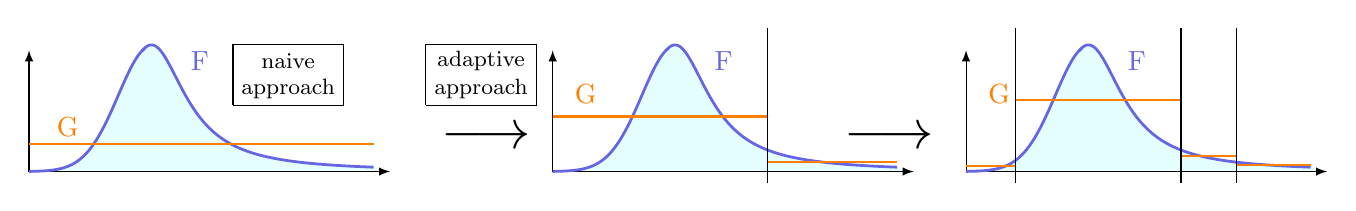
\begin{tikzpicture}[scale=0.7,declare function={
    %%cauchy distrib
    c1 = 6/10;
    c2 = 4/10;
    seuil = c1/(c1+c2);
    a1 = 0.1;
    a2 = 0.2;
    x01 = 0.8;
    x02 = 2.9;
    cauchyMass1(\x) = c1*a1/( pi*( pow(a1,2) + pow((\x-x01),2) ));
    cauchyMass2(\x) = c2*a2/( pi*( pow(a2,2) + pow((\x-x02),2) ));
    loinormale(\x) = c2*exp(-pow((\x-x02),2)/0.05);
    loinormale2(\x) = c2*exp(-pow((\x-x02-1.5),2)/0.3);
      indicatorFunction(\x) = exp(-pow(\x-3,2)/6);
      %%params
      firstVerticalSplitX = 1;
      lastVerticalSplitX = 5.7;
      verticalDashedSplitX = 2.3;
      verticalSplitX = 4;
      lowHorizontalDashedSplitY = 4.5;
      highHorizontalDashedSplitY = 5.5;
      coeffHomothety = 3.8;
      homothetyBone = -1.7;
      homothetyBtwo = -14;
    },
]
  \definecolor{niceblue}{rgb}{0.4,0.4,0.9}
    \definecolor{blue2}{rgb}{0.9,1,1}
\definecolor{ggreen}{rgb}{0.3,0.7,0.4}
\definecolor{orange2}{rgb}{1,0.7,0}

%%%%%%%%%%%%%%%% FIRST curve

\fill [blue2, domain=-7.9:-1.65, variable=\x]
      (-7.9, 1)
      -- plot[samples=200,smooth] ({\x},{
      1.5*coeffHomothety*loinormale((\x-homothetyBone+15)/coeffHomothety)  +1 }
      )
      -- (-1.47, 1)
      -- cycle;
\fill [blue2, domain=-5.8:-1.65, variable=\x]
      (-5.85, 1)
      -- plot[samples=200,smooth] ({\x},{
      1.5*0.633*coeffHomothety*cauchyMass2((\x-homothetyBone+15)/coeffHomothety)
      +1 } )
      -- (-1.47, 1)
      -- cycle;
  \draw[->,>=latex] (-7.9,1) to (-7.9,3.2);
  \draw[->,>=latex] (-7.9,1) to (-1.35,1);
  \draw [domain=-7.9:-5.8, scale=1, color=niceblue, line width=1pt]
  plot[samples=200,smooth] (\x,{
  1.5*coeffHomothety*loinormale((\x-homothetyBone+15)/coeffHomothety)  +1} );
  \draw [domain=-5.85:-1.65, scale=1, color=niceblue, line width=1pt]
  plot[samples=200,smooth] (\x,{
  1.5*0.633*coeffHomothety*cauchyMass2((\x-homothetyBone+15)/coeffHomothety)
  +1} );

  %% splits
  \draw[color=orange,thick] (-7.9,1.5) -- (-1.65,1.5);

  \node[color=orange] at (-7.2,1.8){G};
  \node[color=niceblue] at (-4.8,3){F};

  \node at (-3.2,3){\footnotesize naive};
  \node at (-3.2,2.5){\footnotesize approach};
  \draw (-4.2,2.2) -- (-2.2,2.2) -- (-2.2,3.3) -- (-4.2,3.3) -- (-4.2,2.2);


\node at (0.3,3){\footnotesize adaptive};
  \node at (0.3,2.5){\footnotesize approach};
  \draw (-0.7,2.2) -- (1.3,2.2) -- (1.3,3.3) -- (-0.7,3.3) -- (-0.7,2.2);
    \node at (0.4,1.6) {\scalebox{2}{$\longrightarrow$}};


%%%%%%%%%%%%%%%% second curve

\fill [blue2, domain=1.6:7.95, variable=\x]
      (1.6, 1)
      -- plot[samples=200,smooth] ({\x},{
      1.5*coeffHomothety*loinormale((\x-homothetyBone+5.5)/coeffHomothety)  +1
      } )
      -- (8.03, 1)
      -- cycle;
\fill [blue2, domain=3.65:7.85, variable=\x]
      (3.65, 1)
      -- plot[samples=200,smooth] ({\x},{
      1.5*0.633*coeffHomothety*cauchyMass2((\x-homothetyBone+5.5)/coeffHomothety)
      +1 } )
      -- (8.03, 1)
      -- cycle;
  \draw[->,>=latex] (1.6,1) to (1.6,3.2);
  \draw[->,>=latex] (1.6,1) to (8.15,1);
  \draw [domain=1.6:3.7, scale=1, color=niceblue, line width=1pt]
  plot[samples=200,smooth] (\x,{
  1.5*coeffHomothety*loinormale((\x-homothetyBone+5.5)/coeffHomothety)  +1} );
  \draw [domain=3.65:7.85, scale=1, color=niceblue, line width=1pt]
  plot[samples=200,smooth] (\x,{
  1.5*0.633*coeffHomothety*cauchyMass2((\x-homothetyBone+5.5)/coeffHomothety)
  +1} );


\node[color=niceblue] at (4.7,3){F};


\draw[color=orange,thick] (1.6,2) -- (5.5,2);
\draw[color=orange,thick] (5.5,1.17) -- (7.85,1.17);
     \node[color=orange] at (2.2,2.4){G};

  %% splits
  \draw (5.5,0.8) -- (5.5,3.6);


  %%%%%%%%%%%%%%%%%% third curve

\fill [blue2, domain=9.1:15.45, variable=\x]
      (9.1, 1)
      -- plot[samples=200,smooth] ({\x},{
      1.5*coeffHomothety*loinormale((\x-homothetyBone-2)/coeffHomothety)  +1 }
      )
      -- (15.53, 1)
      -- cycle;
\fill [blue2, domain=11.15:15.35, variable=\x]
      (11.15, 1)
      -- plot[samples=200,smooth] ({\x},{
      1.5*0.633*coeffHomothety*cauchyMass2((\x-homothetyBone-2)/coeffHomothety)
      +1 } )
      -- (15.53, 1)
      -- cycle;
  \draw[->,>=latex] (9.1,1) to (9.1,3.2);
  \draw[->,>=latex] (9.1,1) to (15.65,1);
  \draw [domain=9.1:11.2, scale=1, color=niceblue, line width=1pt]
  plot[samples=200,smooth] (\x,{
  1.5*coeffHomothety*loinormale((\x-homothetyBone-2)/coeffHomothety)  +1} );
  \draw [domain=11.15:15.35, scale=1, color=niceblue, line width=1pt]
  plot[samples=200,smooth] (\x,{
  1.5*0.633*coeffHomothety*cauchyMass2((\x-homothetyBone-2)/coeffHomothety)
  +1} );

\node[color=niceblue] at (12.2,3){F};

    \node at (7.7,1.6) {\scalebox{2}{$\longrightarrow$}};

\draw[color=orange,thick] (9.1,1.1) -- (10,1.1);
\draw[color=orange,thick] (10,2.3) -- (13,2.3);
\draw[color=orange,thick] (13,1.28) -- (14,1.28);
\draw[color=orange,thick] (14,1.12) -- (15.35,1.12);
     \node[color=orange] at (9.7,2.4){G};

  %% splits
  \draw (13,0.8) -- (13,3.6);
\draw (14,0.8) -- (14,3.6);
\draw (10,0.8) -- (10,3.6);

\end{tikzpicture}}
  \caption[Outliers distribution $G$ in the naive and adaptive approach.
  ]{Outliers distribution $G$ in the naive and adaptive approach.  In the naive
  approach, $G$ does not depends on the tree and is constant on the input
  space. In the adaptive approach the distribution depends on the inlier
  distribution $F$ through the tree. The outliers density is constant and equal
  to the average of $F$ on each node before splitting it.
  \label{ocrf:fig:outlier_density}}
\end{figure*}
%
% \begin{figure*}[!ht]
%   \centering
%   \includegraphics[width=1.\linewidth]{outlier_density.png}
%   \caption{\small Outliers distribution $G$ in the naive and adaptive
%   approach.  In the naive approach, $G$ does not depends on the tree and is
%   constant on the input space. In the adaptive approach the distribution
%   depends on the inlier distribution $F$ through the tree. The outliers
%   density is constant and equal to the average of $F$ on each node before
%   splitting it.  %Note that $G$ is tightly concentrated around the inliers,
%   as required in high dimension.  %In the case of more than one tree, the
%   resulting outlier distribution is then the average of such tree-specific
%   densities.  } \label{ocrf:fig:outlier_density}
% \end{figure*}
%
As one does not observe the second-class (outliers), $n_t'$ needs to be
defined. In the naive approach below, it is defined as $n_t'\colonequals n'
\Leb(\mathcal{X}_t) / \Leb(\mathcal{X})$, where $n'$ is the assumed total
number of --hidden-- outliers.
%
In the adaptive approach hereafter, it is defined as $n_t' \colonequals \gamma
n_t$, with typically $\gamma=1$. Thus, the class ratio $\gamma_t \colonequals
n_t'/n_t$ is well defined in both approaches and in the naive approach, goes to
$0$ when $\Leb(\mathcal{X}_t) \to 0$ while it is maintained constant
% $\gamma_t \equiv$ to
to $\gamma$ in the adaptive one.

\subsubsection{Naive approach}
A naive approach to extend the Gini splitting criterion to the one-class
setting is to assume a  uniform distribution for the second class (outliers),
and to replace their number $n_t'$ in node $t$ by the expectation $n'
\Leb(\mathcal{X}_t) / \Leb(\mathcal{X})$, where $n'$ denotes the total number
of outliers (for instance, it can be chosen as a proportion of the number of
inliers).
%
The problem with this approach appears when the dimension is \emph{not small}.
As mentioned in the introduction (curse of dimensionality), when actually
generating $n'$ uniform outliers on $\mathcal{X}$, the probability that a node
(sufficiently small to yield a good precision) contains at least one of them is
very close to zero. That is why data-dependent distributions for the outlier
class are often considered \citep{Desir13, Shi2012}.
%
Taking the expectation $n' \Leb(\mathcal{X}_t) / \Leb(\mathcal{X})$ to replace
the number of points in node $t$ does not solve the curse of dimensionality
mentioned in the introduction: the volume proportion
$L_t\colonequals\Leb(\mathcal{X}_t) / \Leb(\mathcal{X})$ is very close to $0$
for nodes $t$ deep in the tree, especially in large dimension.
%
In addition, we typically grow trees on sub-samples of the input data, meaning
that even the root node of the trees may be very small compared to the
hyper-rectangle containing all the input data.
%
An other problem is that the Gini splitting criterion is skew-sensitive
\citep{Flach2003}, and has here to be apply on nodes $t$ with $0 \simeq n_t'
\ll n_t$. When trying empirically this approach, we observe that splitting such
nodes produces a child containing (almost) all the data (see
\cref{sec:ocrf:theory}).
%
\begin{example}
    To illustrate the fact that the volume proportion
    \begin{dmath*}
        L_t\colonequals \frac{\Leb(\mathcal{X}_t)}{\Leb(\mathcal{X})}
    \end{dmath*}
    becomes very close to zero in large dimension for lots of nodes $t$ (in
    particular the leaves), suppose for the sake of simplicity that the input
    space is $\mathcal{X} = [0,1]^d$. Suppose that we are looking for a rough
    precision of $1/2^3=0.125$ in each dimension, \acs{ie}~a unit cube
    precision of $2^{-3d}$.  To achieve such a precision, the splitting
    criterion has to be used on nodes/cells $t$ of volume of order $2^{-3d}$,
    namely with $L_t = 1/2^{3d}$.  Note that if we decide to choose $n'$ to be
    $2^{3d}$ times larger than the number of inliers in order that $n' L_{t}$
    is not negligible \acs{wrt}~the number of inliers, the same --reversed--
    problem of unbalanced classes appears on nodes with small depth.
\end{example}

\subsubsection{Adaptive approach}
Our solution is to remove the uniform assumption on
the outliers, and to choose their distribution adaptively in such a way it is
tightly concentrated around the inlier distribution. Formally, the idea is to
maintain constant the class ratio $\gamma_t \colonequals n_t' / n_t$ on each
node $t$: before looking for the best split, we update the number of outliers
to be equal (up to a scaling constant $\gamma$) to the number of inliers, $n_t'
= \gamma n_t$, \acs{ie}~$\gamma_t \equiv \gamma$. These --hidden-- outliers are
uniformly distributed on node $t$. The parameter $\gamma$ is typically set to
$\gamma = 1$, see suppl. \Cref{supp:gamma_interpretation} for a discussion on
the relevance of this choice (in a nutshell, $\gamma$ has an influence on
optimal splits).
%
\pgfmathsetseed{7}
\begin{figure*}[ht!]
\center
\resizebox{\textwidth}{!}{%
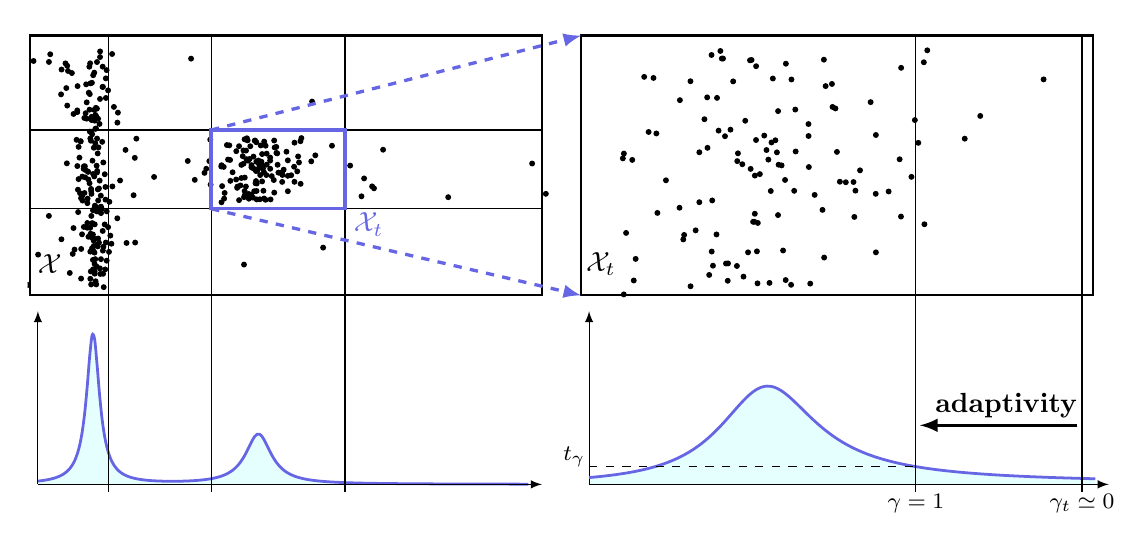
\begin{tikzpicture}[declare function={%
    %%cauchy distrib
    c1 = 6/10;
    c2 = 4/10;
    seuil = c1/(c1+c2);
    a1 = 0.1;
    a2 = 0.2;
    x01 = 0.8;
    x02 = 2.9;
    cauchyMass1(\x) = c1*a1/( pi*( pow(a1,2) + pow((\x-x01),2) ));
    cauchyMass2(\x) = c2*a2/( pi*( pow(a2,2) + pow((\x-x02),2) ));
      cauchyRepFuncInv1(\x) = a1*tan( 3.142*(\x-0.5) r) + x01;
      cauchyRepFuncInv2(\x) = a2*tan( 3.142*(\x-0.5) r) + x02;
      indicatorFunction(\x) = exp(-pow(\x-3,2)/6);
      %%params
      firstVerticalSplitX = 1;
      lastVerticalSplitX = 5.7;
      verticalDashedSplitX = 2.3;
      verticalSplitX = 4;
      lowHorizontalDashedSplitY = 4.5;
      highHorizontalDashedSplitY = 5.5;
      coeffHomothety = 3.8;
      homothetyBone = -1.7;
      homothetyBtwo = -14;
    },
]
  \definecolor{niceblue}{rgb}{0.4,0.4,0.9}
    \definecolor{blue2}{rgb}{0.9,1,1}

    %%% draw area
    \clip (-0.03,0.5) rectangle (13.8,6.8);

    %%% TOP RECTANGLES
    \draw[thick] (0,3.4) rectangle (6.5,6.7);
    \draw[thick] (7,3.4) rectangle (13.5,6.7);
    \node at (0.25,3.8) {$\mathcal{X}$};
    \node at (7.25,3.8) {$\mathcal{X}_t$};
    \node[color=niceblue] at (verticalSplitX+0.3,lowHorizontalDashedSplitY-0.2)
    {$\mathcal{X}_t$};

    %%%%%%%%%%%%%%%%%% LEFT PART
    %%% points sampling
    \foreach \x in {1,2,...,350}{%
    \pgfmathsetmacro{\seuil}{c1/(c1+c2)}
    \pgfmathsetmacro{\aleatorio}{rnd}
    \pgfmathsetmacro{\rndCauchy}{\aleatorio>seuil ? 0 : 1 }
    \pgfmathsetmacro{\abscissePoint}{\rndCauchy*cauchyRepFuncInv1(rand) +
    (1-\rndCauchy)*cauchyRepFuncInv2(rand)}
    \pgfmathsetmacro{\ordinatePoint}{\rndCauchy*(1.5*rand+5) +
    (1-\rndCauchy)*(rand*0.4+5)}
    \pgfmathsetmacro{\abscissePointFiltered}{ \abscissePoint>6.6 ? -10 :
    \abscissePoint }
    \pointSampled{\abscissePointFiltered,\ordinatePoint}
    \pgfmathsetmacro{\rightEnough}{\abscissePoint>verticalDashedSplitX ? true :
    false }
    \pgfmathsetmacro{\leftEnough}{\abscissePoint<verticalSplitX ? true : false }
    \pgfmathsetmacro{\highEnough}{\ordinatePoint>lowHorizontalDashedSplitY ?
    true : false}
    \pgfmathsetmacro{\lowEnough}{\ordinatePoint<highHorizontalDashedSplitY ?
    true : false}
    \pgfmathsetmacro{\newAbscisse}{\rightEnough && \leftEnough && \highEnough
    && \lowEnough ? \abscissePoint*coeffHomothety + homothetyBone : -10  }
    \pointSampled{\newAbscisse,\ordinatePoint*coeffHomothety + homothetyBtwo}
  }


  %% curve
 \fill [blue2, domain=0.1:6.33, variable=\x]
      (0.1, 1)
      -- plot[samples=200,smooth] ({\x},{cauchyMass1(\x) + cauchyMass2(\x) +1}
      )
      -- (6.33, 1)
      -- cycle;
  \draw [domain=0.1:6.33, scale=1, color=niceblue, line width=1pt, fill=blue2]
  plot[samples=200,smooth] (\x,{cauchyMass1(\x) + cauchyMass2(\x) +1});
  %% axis
  \draw[->,>=latex] (0.1,1) to (0.1,3.2);
  \draw[->,>=latex] (0.1,1) to (6.5,1);

  %% splits
  \draw (firstVerticalSplitX,0.9) -- (firstVerticalSplitX,6.7); % gamma=10
  \draw (verticalSplitX,0.9) -- (verticalSplitX,6.7); % gamma=1
  %\draw (lastVerticalSplitX,0.9) -- (lastVerticalSplitX,6.7); % gamma=0.1
  %\node[below] at (firstVerticalSplitX,1){\footnotesize $\gamma=10$};
  %\node[below] at (verticalSplitX,1){\footnotesize $\gamma=1$};
  %\node[below] at (lastVerticalSplitX+0.5,1){\footnotesize $\gamma=0.1$};

  \draw (verticalDashedSplitX,0.9) -- (verticalDashedSplitX,6.7);
  \draw (0,lowHorizontalDashedSplitY) -- (6.5,lowHorizontalDashedSplitY);
  \draw (0,highHorizontalDashedSplitY) -- (6.5,highHorizontalDashedSplitY);

  %% ZOOM
  \draw[very thick, color=niceblue]
  (verticalDashedSplitX,lowHorizontalDashedSplitY) rectangle
  (verticalSplitX,highHorizontalDashedSplitY);
  \draw[very thick, dashed, color=niceblue,->,>=latex]
  (verticalDashedSplitX,highHorizontalDashedSplitY) -- (7,6.7);
  \draw[very thick, dashed, color=niceblue,->,>=latex]
  (verticalDashedSplitX,lowHorizontalDashedSplitY) -- (7,3.4);


  %%%%%%%%%%%%%%%%%% RIGHT PART second curve
  \fill [blue2, domain=7.1:13.53, variable=\x]
      (7.1, 1)
      -- plot[samples=200,smooth] ({\x},{%
      indicatorFunction((\x-7)/5)*coeffHomothety*1.5*cauchyMass2((\x-homothetyBone)/coeffHomothety)
      +1 } )
      -- (13.53, 1)
      -- cycle;
  \draw[->,>=latex] (7.1,1) to (7.1,3.2);
  \draw[->,>=latex] (7.1,1) to (13.7,1);
  \draw [domain=7.1:13.53, scale=1, color=niceblue, line width=1pt]
  plot[samples=200,smooth] (\x,{%
  indicatorFunction((\x-7)/5)*1.5*coeffHomothety*cauchyMass2((\x-homothetyBone)/coeffHomothety)
  +1} );

  %% splits
  \draw (verticalSplitX+7.25,0.9) -- (verticalSplitX+7.25,6.7); % gamma=1
  \draw (13.36,0.9) -- (13.36,6.7); % gammat
  \node[below] (gammaone) at (verticalSplitX+7.25,1){\footnotesize $\gamma=1$};
  \node[below] (gammat) at (13.36,1){\footnotesize $\gamma_t \simeq 0$};
  \draw[dashed] (7.1,1.23) -- (verticalSplitX+7.25,1.23);
  \node[right] at (6.65,1.35){\footnotesize $t_{\gamma}$};

  \draw[->,>=latex, very thick] (13.3,1.75) to (verticalSplitX+7.3,1.75);
  \node at (verticalSplitX+8.4,2)  {\textbf{adaptivity}};

\end{tikzpicture}}
\caption[Adaptative splitting criteria]{The left part represents
the dataset under study and the underlying density.  The node $\mathcal{X}_t$
obtained after some splits is illustrated in the right part of this figure:
without the proposed adaptive approach, the class ratio $\gamma_t$ becomes too
small and yields poor splits
%(normal data are condensed on a very small volume)
(all the data are in the \say{inlier side} of the split, which thus does not
discriminate at all).  Contrariwise, setting $\gamma$ to one, \acs{ie}~using
the adaptive approach, is far preferable.
%Note that a given $\gamma$ corresponds to a level set $t_{\gamma}$.
 \label{ocrf:fig:split_alpha}}
\end{figure*}
\paragraph{}
With this methodology, one cannot derive a one-class version of the Gini index
\cref{ocrf:eq:gini}, but we can define a one-class version of the proxy of the
impurity decrease \cref{ocrf:tc_proxy}, by simply replacing $n_{t_L}'$
(respectively $n_{t_R}'$) by $n_t' \lambda_L$ (resp. $n_t' \lambda_R$), where
$\lambda_L \colonequals \Leb(\mathcal{X}_{t_L}) / \Leb(\mathcal{X}_{t})$ and
$\lambda_R \colonequals \Leb(\mathcal{X}_{t_R}) / \Leb(\mathcal{X}_{t})$ are
the volume proportion of the two child nodes
%
\begin{dmath}
    \label{ocrf:oc_proxy_ad2}
    I_G^{OC-ad}(t_L, t_R)= \frac{n_{t_L} \gamma n_t \lambda_L}{n_{t_L} + \gamma
    n_t \lambda_L} + \frac{n_{t_R} \gamma n_t \lambda_R}{n_{t_R} + \gamma n_t
    \lambda_R}.
\end{dmath}
%
Minimization of the one-class Gini improvement proxy \cref{ocrf:oc_proxy_ad2}
is illustrated in \cref{ocrf:fig:split_alpha}.
%and \Cref{ocrf:fig:split_two_modes}.
Note that $n_t'\lambda_L$ (resp. $n_t'\lambda_R$) is the expectation of the
number of uniform  observations (on $\mathcal{X}_t$) among $n_t'$ (fixed to
$n_t' = \gamma n_t$) falling into the left (respectively right) node.
\paragraph{}
Choosing the split minimizing $I_G^{OC-ad}(t_L, t_R)$ at each step of the tree
building process, corresponds to generating $n_t' = \gamma n_t$ outliers each
time the best split has to be chosen for node $t$, and then using the classical
two-class Gini proxy \cref{ocrf:tc_proxy}. The only difference is that
$n_{t_L}'$ and $n_{t_R}'$ are replaced by their expectations
$n_t'\lambda_{t_L}$ and $n_t'\lambda_{t_R}$ in our method.

\subsubsection{Resulting outlier distribution}
\Cref{ocrf:fig:outlier_density} shows the corresponding outlier density $G$ (we
drop the dependence in the number of splits to keep the notations uncluttered).
Note that $G$ is a piece-wise constant approximation of the inlier distribution
$F$. Considering the Neyman-Pearson test $X \sim F$ versus $X \sim G$ instead
of $X \sim F$ versus $X \sim \mathcal{U}$ may seem surprising at first sight.
Let us try to give some intuition on why this works in practice. First, there
exists (at each step) $\epsilon>0$ such that $G>\epsilon$ on the entire input
space, since the density $G$ is constant on each node and equal to the average
of $F$ on this node \emph{before splitting it}. If the average of $F$ was
estimated to be zero (no inlier in the node), the node would obviously not have
been split, from where the existence of $\epsilon$.
%
Thus, at each step, one can also view $G$ as
% Note that $G$ on some leaf $t_m$ with parents $t_0, \ldots, t_{m-1}$ takes
% the form $G_{|t_m} = \sum_{j=0}^{m} \int_{\mathcal{X}_{t_i}} F =
% 1/\leb{\mathcal{X}} + \sum_{j=1}^{m} \int_{\mathcal{X}_{t_i}} F $
a piece-wise approximation of $F_\epsilon := (1 - \epsilon) F + \epsilon
\mathcal{U}$, which is a mixture of $F$ and the uniform distribution. %
($\epsilon$ depending on the step/number of splits) Yet, one can easily show
that optimal tests for the Neyman-Pearson problem $H_0: X \sim F$ vs. $H_1: X
\sim F_\epsilon$ are identical to the optimal tests for $H_0: X \sim F$ vs.
$H_1: X \sim \mathcal{U}$, since the corresponding likelihood ratios are
related by a monotone transformation, see \citet{Scott2009} for instance (in
fact, this reference shows that these two problems are even equivalent in terms
of consistency and rates of convergence of the learning rules). An other
intuitive justification is as follows. In the first step, the algorithm tries
to discriminate $F$ from $\mathcal{U}$. When going deeper in the tree, splits
manage to discriminate $F$ from a (more and more accurate) approximation of
$F$. Asymptotically, splits become irrelevant since they are trying to
discriminate $F$ from itself (a perfect approximation, $\epsilon \to 0$).
%
%\begin{remark}({\sc By-product: Efficiently generating outliers})
\begin{remark}({Consistency with the two-class framework})
    Consider the following method to generate outliers --tightly concentrated
    around the support of the inlier distribution.
    % it suffices to generate them as described above, recursively during the
    % tree building process.
    Sample uniformly $n'= \gamma n$ outliers on the rectangular cell containing
    all the inliers. Split this root node using classical two-class impurity
    criterion (\acs{eg}~minimizing \cref{ocrf:tc_proxy}). Apply recursively the
    three following steps: for each node $t$, remove the potential outliers
    inside  $\mathcal{X}_t$, re-sample $n_t'=\gamma n_t$ uniform outliers on
    $\mathcal{X}_t$, and use the latter to find the best split using
    \Cref{ocrf:tc_proxy}.
    %, and start again on $\mathcal{X}_{t_L}$ and $\mathcal{X}_{t_R}$.
    Then, each optimization problem \cref{ocrf:tc_proxy} we have solved is
    equivalent (in expectation) to its one-class version
    \cref{ocrf:oc_proxy_ad2}. In other words, by generating outliers
    adaptively, we can recover (in average) a tree grown using the one-class
    impurity, from a tree grown using the two-class impurity.
    %the one-class splitting criterion promoted in this paper can be recovered
    %from the two-class one, when generating the outliers adaptively.
\end{remark}

\begin{remark}({Extension to other impurity criteria})
    Our extension to the one-class setting also applies to other impurity
    criteria. For instance, in the case of the Shannon entropy defined in the
    two-class setup by
    %\begin{align*}
    %\label{ocrf:eq:shannon}
    \begin{dmath*}
        i_S(t) = \frac{n_t}{n_t + n_t'} \log_2 \frac{n_t + n_t'}{n_t} +
        \frac{n_t'}{n_t + n_t'} \log_2 \frac{n_t + n_t'}{n_t'},
    \end{dmath*}
    %\end{align*}
    the one-class impurity improvement proxy becomes
    %\begin{align*}
    %\label{ocrf:eq:one_class_shannon_proxy}
    \begin{dmath*}
        I_S^{OC-ad}(t_L, t_R) = n_{t_L} \log_2 \frac{n_{t_L} + \gamma n_t
        \lambda_L}{n_{t_L}} + n_{t_R} \log_2 \frac{n_{t_R} + \gamma n_t
        \lambda_R}{n_{t_R}}.
    \end{dmath*}
    %\end{align*}
\end{remark}
%
%
\subsection{Prediction: scoring function of the forest}
%: a majority vote with one single candidate?}
\label{ocrf:sec:prediction}
 Now that \acp{RF} can be grown in the one-class setting using the one-class
 splitting criterion, the forest has to return a prediction adapted to this
 framework.  In other words we also need to extend the concept of majority
 vote.
%
\begin{figure}[htb]
    \centering
    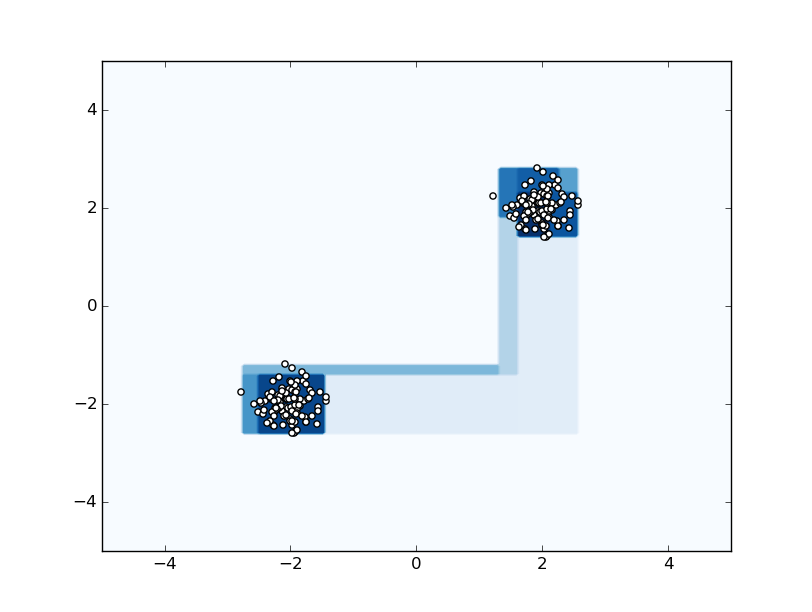
\includegraphics[width=\textwidth]{./gfx/oneclassrf.png}
    \caption[One Class Random Forest level-sets]{\ac{OneClassRF} with one tree,
    level-sets of the scoring function. \label{ocrf:fig:oneclassrf}}
\end{figure}

Most usual one-class (or more generally anomaly detection) algorithms actually
provide more than just a level-set estimate or a predicted label for any new
observation, abnormal versus normal. Instead, they return a real valued
function, termed \emph{scoring function}, defining a preorder/ranking on the
input space. Such a function $s: \mathbb{R}^d \to \mathbb{R}$ allows to rank
any observations according to their supposed \say{degree of abnormality}.
Thresholding it provides level-set estimates, as well as a decision rule that
splits the input space into inlier/normal and outlier/abnormal regions.
%
%We thus adapt the majority vote to the one-class setting by defining the
%scoring function of a forest.
%
%We propose three natural scoring functions of a forest.
The scoring function $s(x)$ we use is the one defined in \citet{Liu2008} in
view of its established high performance. It is a decreasing function of the
average depth of the leaves containing $x$ in the forest.
%, `if the trees were fully grown':
An average term is added to each node containing more than one sample, say
containing $N$ samples. This term $c(N)$ is the average depth of an extremely
randomized tree \citep{Geurts2006} (\acs{ie}~built without minimizing any
criterion, by randomly choosing one feature and one uniform value over this
feature to split on) on $N$ samples. Formally,
\begin{dmath}
    \label{ocrf:eq:scoring3}
    \log_2 s(x) = -\left(\sum_{t \text{~leaves}} \mathds{1}_{\Set{x \in t}} d_t
    + c(n_t)\right) / c(n),
\end{dmath}
where $d_t$ is the depth of node $t$, and $c(n) = 2H(n - 1) - 2(n - 1)/n$,
$H(i)$ being the harmonic number. Alternative scoring functions can be defined
for this one-class setting (see \cref{supp:scoring_functions}).
%
%
%
\subsection{OneClassRF: a Generic One-Class Random Forest algorithm}
Let us summarize the One Class Random Forest algorithm, based on generic
\acp{RF} \citep{Breiman2001}. It has $6$ parameters, namely
\texttt{max\textunderscore samples}, \texttt{max\textunderscore
features\textunderscore tree}, \texttt{max\textunderscore
features\textunderscore node}, $\texttt{gamma}$, \texttt{max\textunderscore
depth}, \texttt{n\textunderscore trees}.
%
\begin{table*}[ht]
    \caption{Original datasets characteristics}
    \label{ocrf:table:data}
    \centering
    \footnotesize
    %\tabcolsep=0.08cm
    \begin{tabularx}{\textwidth}{lccXl}
        \toprule
        Datasets        & nb of samples      & nb of features     &
       anomaly class      &                   \\
        \midrule
        adult       & 48842              & 6                  &    class
        '$>50K$' &      (23.9\%)      \\
        annthyroid  & 7200               & 6                  &    classes
        $\neq$ 3 &        (7.42\%)    \\
        arrhythmia  & 452                & 164                &    classes
        $\neq$ 1 (features 10-14 removed)&  (45.8\%)          \\
        forestcover & 286048             & 10                 &    class 4
        (versus  class 2 )                  &           (0.96\%) \\
        http        & 567498             & 3                  &      attack &
        (0.39\%)        \\
        ionosphere  & 351                & 32                 &    bad &
        (35.9\%)     \\
        pendigits   & 10992              & 16                 &    class 4 &
        (10.4\%)    \\
        pima        & 768                & 8                  &    pos (class
        1) &        (34.9\%)    \\
        shuttle     & 85849              & 9                  &      classes
        $\neq$ 1 (class 4 removed)     &  (7.17\%)          \\
        smtp        & 95156              & 3                  &      attack &
        (0.03\%)        \\
        spambase    & 4601               & 57                 &    spam &
        (39.4\%) \\
        wilt        & 4839               & 5                  &    class `w'
        (diseased trees)               &    (5.39\%)        \\
        \bottomrule
    \end{tabularx}
\end{table*}
\paragraph{}
Each tree is classically grown on a random subset of both the input samples and
the input features \citep{Ho1998, Panov2007}.  This random subset is a
sub-sample of size \texttt{max\textunderscore samples}, with
\texttt{max\textunderscore features\textunderscore tree} variables chosen at
random without replacement (replacement is only done after the tree is grown).
The tree is built by minimizing \cref{ocrf:oc_proxy_ad2} for each split, using
parameter $\gamma$ (recall that $n_t' \colonequals \gamma n_t$), until either
the maximal depth \texttt{max\textunderscore depth} is achieved or the node
contains only one point.
% define a large number of geometric features and search over a random
% selection of these for the best split at each node
Minimizing \cref{ocrf:oc_proxy_ad2} is done as introduced in \citet{Amit1997}:
at each node, we search the best split over a random selection of features with
fixed size $max\textunderscore features\textunderscore node$.
%
The forest is composed of a number $n\textunderscore trees$ of trees. The
predicted score of a point $x$ is given by $s(x)$, with $s$ defined by
\Cref{ocrf:eq:scoring3}.
%SH (copier en suppl mat) As an illustration, Figure~\Cref{ocrf:fig:oneclassrf}
%represents the level set of the scoring function produced by OneClassRF, with
%only one tree ($n\textunderscore trees$$=1$) of maximal depth
%$max\textunderscore depth$=4, without sub-sampling, and using the Gini-based
%one-class splitting criterion with
%$\gamma=1$.
Remarks on alternative stopping criteria and variable importances are available
in \cref{supp:stopping_criteria}.
\paragraph{}
\Cref{ocrf:fig:oneclassrf} represents the level sets of the scoring function
produced by \ac{OneClassRF}, with only one tree
% ($n\textunderscore trees$$=1$)
of maximal depth $4$,
% $max\textunderscore depth$=4
without sub-sampling, and using the Gini-based one-class splitting criterion
with $\gamma=1$.
%
%
% \begin{remark}({\sc Underlying Level-Set estimation}) As mentionned above,
% the link between $\gamma$ and the level of the level-set estimate induced by
% the split is difficult to exhibit, as well as how it repercutes into the
% level of the global level-set estimate.  Intuitively, $\gamma$ plays the same
% role as parameter $\nu$ for the OCSVM in its $\nu$-soft margin formulation.
% OCSVM also returns a scoring function (inducing an infinite number of
% level-sets), but which seeks to be optimal for estimating a particular
% level-set (corresponding to a particular thresholding of the scoring
% function) whose level can explicitely be controlled by $\nu$.  However, we
% are not able to derive an explicit relation, as it exists for the OCSVM,
% between the targeted level set and $\gamma$. Note that this does not mean
% that we are not able to estimate any arbitrary level-set. It only means that
% we do not know for which level, the scoring function outputed by OneClassRF
% originally seeks to be optimal.  \end{remark}
%
%
%by \Cref{ocrf:eq:scoring1}, \Cref{ocrf:eq:scoring2} or
%\Cref{ocrf:eq:scoring3}.  \paragraph{Description of the OneClassRF algorithm.}
%Now that we have exposed the one-class splitting rule to grow the trees, as
%well as the forest output replacing the majority vote, the one-class random
%forest algorithm promoted here is described as follows. %similar to Breiman's
%approach, see \cite{Breiman2001}.  % Let us denote by \ttt{X} the input data.
%In its most generic version, it has five parameters, $max\textunderscore
%samples$, $max\textunderscore features$, $n\textunderscore estimators$,
%$max\textunderscore depth$ and $\gamma$.  Each tree is classicaly grown on a
%random subset of both the input samples and the input variables,
%see~\cite{Ho1998, Panov2007}. This random subset is a sub-sample of size
%$max\textunderscore samples$, with $max\textunderscore features$ variables
%chosen at random without replacement (replacement is only done after the tree
%is grown). The tree is built by minimizing \Cref{ocrf:oc_proxy_ad2} at each
%step using parameter $\gamma$, until the maximal depth $max\textunderscore
%depth$ is achieved. The forest is composed of a number $n\textunderscore
%estimators$ of trees. The predicted score of a point $x$ is given by
%\Cref{ocrf:eq:scoring}, namely the average (over the trees) of
%$n_t/\leb(\mathcal{X}_t)$, where $t$ is the leaf node (of the tree considered)
%containing $x$.  % \begin{algorithm}[OneClassRF.fit]~\\ % \begin{pythoncode} %
%Inputs: X % Parameters: max_samples, max_features, n_estimators, max_depth %
%Output: A set of n_estimators trees.  % \end{pythoncode} % \end{algorithm}
%\begin{remark}({\sc Extremely Randomized Trees}) In the case of extremely
%randomized trees (see \cite{Geurts2006}), namely trees grown totally randomly
%as used in Isolation Forest (\cite{Liu2008}), no splitting criterion is needed
%so that no impurity function is used. The one class version of the
% majority vote can still be used in this case, which yields a scoring function
% of the form $s(x) = \sum_t \mathds{1}_{\{\Omega_t \}}
% \frac{N_t}{\leb(\Omega_t)}$. XXX benchmark on this algo? (easy: iforest with
% score from OCSVM) \end{remark}
%XXX sklearn exemple with OneClassRF with different alpha
%

\section{Benchmarks}
\label{ocrf:sec:benchmark}
%
In this section, we compare the \ac{OneClassRF} algorithm described above to
seven state-of-art anomaly detection algorithms: the \ac{iForest} algorithm
\citep{Liu2008}, a one-class \acp{RF} algorithm based on sampling a
second class \ac{OCRFsampling} \citep{Desir13}, \acf{OCSVM}
\citep{Scholkopf2001}, \acf{LOF} \citep{Breunig2000LOF}, Orca \citep{Bay2003},
\acf{LSAD} \citep{Quinn2014}, \acf{RFC} \citep{Shi2012}.
%We have used default parameters for these algorithms, as detailed in
%supplementary material.
%
\subsection{Default parameters of OneClassRF}
The default parameters taken for our algorithm are the followings.
%
\begin{itemize}
    \item \texttt{max\textunderscore samples} is fixed to $20\%$ of the
    training sample size (with a minimum of $100$);
    \item \texttt{max\textunderscore features\textunderscore tree} is fixed to
    $50\%$ of the total number of features with a minimum of $5$ (\acs{ie}~each
    tree is built on $50\%$ of the total number of features);
    \item \texttt{max\textunderscore features\textunderscore node} is fixed to
    $5$;
    \item $\gamma$ is fixed to $1$;
    \item \texttt{max\textunderscore depth} is fixed to $\log_2$ (logarithm in
    base $2$) of the training sample size as in \citet{Liu2008};
    \item \texttt{n\textunderscore trees} is fixed to $100$ as in the previous
    reference.
\end{itemize}
%and parameter $s_i$ is set to $s_3$ as defined in \eqref{ocrf:eq:scoring3}.
\paragraph{}
The other algorithms in the benchmark are trained with their recommended
(default) hyper-parameters as seen in their respective paper or author's
implementation. See \cref{supp:hyper_choice} for details.
%
The characteristics of the twelve reference datasets considered here are
summarized in \cref{ocrf:table:data}. They are all available on the \acs{UCI}
repository \citep{Lichman2013} and the preprocessing is done as usually in the
literature (see \cref{supp:dataset_description}).
%
%
\maxdeadcycles=1000
\afterpage{%
\begin{landscape}
    \begin{table}[htb]
        \centering
        \caption{Results for the novelty detection setting.
        %We compare various methods from the state-of-the-art (top line) to
        %OneClassRF over different classical datasets (leftmost column).
        \label{ocrf:table:results-semisupervised}}
        %\scriptsize
        \resizebox{\textheight}{!}{%
        \begin{tabular}{lcccccccccccccccc}
        \toprule
            %
            Datasets & \multicolumn{2}{c }{\ac{OneClassRF}} & \multicolumn{2}{c
            }{\ac{iForest}} & \multicolumn{2}{c }{\ac{OCRFsampling}} &
            \multicolumn{2}{c }{\ac{OCSVM}}& \multicolumn{2}{c }{\ac{LOF}}&
            \multicolumn{2}{c }{Orca}& \multicolumn{2}{c }{\ac{LSAD}}&
            \multicolumn{2}{c }{\ac{RFC}}  \\%& parameters $(\epsilon, k)$\\
        \cmidrule{1-17}
            \acs{AUC}   & \acs{ROC} &  \acs{PR} & \acs{ROC} &  \acs{PR} &
            \acs{ROC} & \acs{PR}  & \acs{ROC} & \acs{PR}  & \acs{ROC} &
            \acs{PR} & \acs{ROC} & \acs{PR}  & \acs{ROC} &  \acs{PR} &
            \acs{ROC} & \acs{PR}  \\
            adult        &        \textbf{0.665} & \textbf{0.278} & 0.661 &
            0.227 & \acs{NA} & \acs{NA} & 0.638 & 0.201 & 0.615 & 0.188 & 0.606
            & 0.218 & 0.647    & 0.258     & \acs{NA} & \acs{NA} \\
            annthyroid   &        \textbf{0.936} & 0.468 & 0.913 & 0.456 &
            0.918 & \textbf{0.532} & 0.706 & 0.242 & 0.832 & 0.446 & 0.587 &
            0.181 &  0.810 & 0.327     & \acs{NA} & \acs{NA} \\
            arrhythmia   &        0.684 & 0.510 & 0.763 & 0.492 & 0.639 & 0.249
            & \textbf{0.922} & \textbf{0.639} & 0.761 & 0.473 & 0.720 & 0.466 &
            0.778 & 0.514     & 0.716 & 0.299 \\
            forestcover  &        0.968 & 0.457 & 0.863 & 0.046 & \acs{NA} &
            \acs{NA} & \acs{NA} & \acs{NA} & \textbf{0.990} & \textbf{0.795} &
            0.946 & 0.558 &  0.952    & 0.166 & \acs{NA} & \acs{NA} \\
            http         &        \textbf{0.999} & \textbf{0.838} & 0.994 &
            0.197 & \acs{NA} & \acs{NA} & \acs{NA} & \acs{NA} & \acs{NA} &
            \acs{NA} & \textbf{0.999} & 0.812 &  0.981    & 0.537     &
            \acs{NA} & \acs{NA} \\
            ionosphere   &        0.909 & 0.643 & 0.902 & 0.535 & 0.859 & 0.609
            & 0.973 & 0.849 & 0.959 & 0.807 & 0.928 & \textbf{0.910} &
            \textbf{0.978} & 0.893     & 0.950 & 0.754 \\
            pendigits    &        0.960 & 0.559 & 0.810 & 0.197 & 0.968 & 0.694
            & 0.603 & 0.110 & 0.983 & 0.827 & \textbf{0.993} & \textbf{0.925} &
            0.983 & 0.752     & \acs{NA} & \acs{NA} \\
            pima         &        0.719 & 0.247 & 0.726 & 0.183 &
            \textbf{0.759} & \textbf{0.266} & 0.716 & 0.237 & 0.700 & 0.152 &
            0.588 & 0.175 &  0.713 & 0.216     & 0.506 & 0.090 \\
            shuttle      &        \textbf{0.999} & \textbf{0.998} & 0.996 &
            0.973 & \acs{NA} & \acs{NA} & 0.992 & 0.924 & \textbf{0.999} &
            0.995 & 0.890 & 0.782 & 0.996    & 0.956     & \acs{NA} & \acs{NA}
            \\ smtp         &        0.922 & 0.499 & 0.907 & 0.005 & \acs{NA} &
            \acs{NA} & 0.881 & \textbf{0.656} & \textbf{0.924} & 0.149 & 0.782
            & 0.142 &  0.877    & 0.381     & \acs{NA} & \acs{NA} \\
            spambase &        \textbf{0.850} & 0.373 & 0.824 & 0.372 & 0.797 &
            \textbf{0.485} & 0.737 & 0.208 & 0.746 & 0.160 & 0.631 & 0.252 &
            0.806 & 0.330     & 0.723 & 0.151 \\
            wilt         &        0.593 & 0.070 & 0.491 & 0.045 & 0.442 & 0.038
            & 0.323 & 0.036 & 0.697 & 0.092 & 0.441 & 0.030 &  0.677    & 0.074
            & \textbf{0.896} & \textbf{0.631} \\
        \cmidrule{1-17}
            average    & \textbf{0.850} & \textbf{0.495} & 0.821 & 0.311 &
            0.769 & 0.410 & 0.749 & 0.410 & 0.837 & 0.462 & 0.759 & 0.454 &
            \textbf{0.850} & 0.450 &  0.758  & 0.385 \\
            \acs{cum} train time & \multicolumn{2}{c }{\textbf{61s}} &
            \multicolumn{2}{c }{68s} & \multicolumn{2}{c }{\acs{NA}} &
            \multicolumn{2}{c }{\acs{NA}}& \multicolumn{2}{c }{\acs{NA}}&
            \multicolumn{2}{c }{2232s}& \multicolumn{2}{c }{73s}&
            \multicolumn{2}{c }{\acs{NA}}  \\
        \bottomrule
        \end{tabular}}
    \end{table}
\end{landscape}}
%
%
\subsection{Results}
All the code is available at \url{https://github.com/ngoix/OCRF}. The
experiments are performed in the novelty detection framework, where the
training set consists of inliers only.
%We removed anomalies from the training data.
No significance level test are given, but experiements or each algorithm are
repeated $10$ times on random training and testing datasets are performed,
yielding averaged \ac{ROC} and \ac{PR} curves whose \acsp{AUC} are summarized
in \cref{ocrf:table:results-semisupervised} (higher is better).
%We use the set of hyper-parameters recommanded in the corresponding reference
%papers.
The training time of each algorithm has been limited (for each experiment among
the $10$ performed for each dataset) to $30$ minutes, where \acs{NA} indicates
that the algorithm could not finish training within the allowed time limit.  In
average on all the datasets, our proposed algorithm \ac{OneClassRF} achieves
both best \acs{AUC} \acs{ROC} and \acs{AUC} \acs{PR} scores (with \acs{LSAD}
for \acs{AUC} \acs{ROC}). It also achieves the lowest cumulative training time.
%
For further insights on the benchmarks \acs{cf}~\cref{supp:further_exp}.
%
%Figures \Cref{ocrf:figNoveltyAUCROC} and \Cref{ocrf:figNoveltyCompTime}
%summarize the results. % from the novelty detection framework, whereas figures
%\Cref{ocrf:figUnsupervAUCROC}, \Cref{ocrf:figUnsupervAUCPR} and
%\Cref{ocrf:figUnsupervCompTime} presents those from the unsupervised one.  In
%the novelty detection settings,
It appears that \ac{OneClassRF} has the best performance on five datasets in
terms of \acs{ROC} \acsp{AUC}, and is also the best in average.
%\footnote{Precision-Recall AUCs have also been computed and are
%available in the supplementary material.},
Computation times (training plus testing) of \ac{OneClassRF} are also very
competitive.
% (see supplementary material).
%In the unsupervised settings, OneClassRF and iForest have similar performances
%in terms of AUCs (ROC and PR), but OneClassRF still uses less computation
%time.
%
%These results are surprising: iForest computation time should be lower since
%it randomly builds trees. The explaination is....
%
% T = np.array([[1.83, 1.19, np.NAN, 16.20, 7.03, 9.42, 1.05, np.NAN],
% [0.39, 0.19, 65.02, 0.54, 1.03, 0.66, 0.31, np.NAN],
% [0.36, 0.12, 9.30, 0.0, 0.04, 0.38, 0.01, 33.17],
% [19.97, 15.86, np.NAN, np.NAN, 59.56, 733.75, 6.18, np.NAN],
% [29.5, 42.25, np.NAN, np.NAN, np.NAN, 1368.83, 51.41, np.NAN],
% [0.36, 0.10, 2.47, 0.0, 0.03, 0.38, 0.0, 12.42],
% [0.67, 0.32, 458.94, 1.35, 1.66, 1.81, 0.42, np.NAN],
% [0.13, 0.10, 5.20, 0.0, 0.12, 0.26, 0.01, 18.12],
% [3.13, 3.87, np.NAN, 95.99, 20.39, 76.24, 7.42, np.NAN],
% [3.99, 3.51, np.NAN, 118.93, 12.11, 38.52, 5.98, np.NAN],
% [0.49, 0.21, 55.71, 0.22, 0.85, 1.49, 0.25, 593.87],
% [0.39, 0.16, 68.29, 0.14, 0.73, 0.46, 0.22, 752.19]])
% np.mean(T, axis=0)
% array([   5.10083333,    5.65666667,           nan,           nan,
%                  nan,  186.01666667,    6.105     ,           nan])
%
%
Experiments in an outlier detection framework (the training set is polluted by
outliers) have also been made (see \cref{sup:outlier_detection}).
%In this case, the anomaly rate is arbitrarily bounded to $10\%$ max (before
%splitting data into training and testing sets).
The anomaly rate is arbitrarily bounded to $10\%$ max (before splitting data
into training and testing sets).
%
%
%
%
\section{Theoretical analysis}
%justification for the one-class splitting criterion}
\label{sec:ocrf:theory}
This section aims at recovering \cref{ocrf:oc_proxy_ad2} from a natural
modeling of the one-class framework, along with a theoretical study of the
problem raised by the naive approach.
\subsection{Underlying model}
\label{ocrf:sec:model} In order to generalize the two-class framework to the
one-class one, we need to consider the population versions associated to
empirical quantities \cref{ocrf:eq:impurity_measure_decrease},
\cref{ocrf:eq:gini} and \cref{ocrf:eq:two_class_proxy}, as well as the
underlying model assumption. The latter can be described as follows.

\subsubsection{Existing Two-Class Model (n, $\boldsymbol{\alpha}$).}
We consider a \acs{rv}~$X:\Omega \to \mathbb{R}^d$ \acs{wrt}~a probability
space $(\Omega, \mathcal{F}, \probability)$. The law of $X$ depends on another
\acs{rv}~$y \in \{0,1\}$, verifying
$\probability\Set{y=1}=1-\probability\Set{y=0}=\alpha$.  We assume that
conditionally on $y=0$, $ X$ follows a law $F$, and conditionally on $y=1$ a
law $G$;
%To summarize:
\begin{dgroup*}
\begin{dmath*}
    X\enskip|\enskip y=0 \quad\sim\quad F, \qquad
    \probability\Set{y=0}=1-\alpha,
\end{dmath*}
\begin{dmath*}
    X\enskip|\enskip y=1 \quad\sim\quad G, \qquad
    \probability\Set{y=1}=\alpha.
\end{dmath*}
\end{dgroup*}
Then, considering
\begin{dmath*}
    p(t_L | t) = \probability\Set{X\in \mathcal{X}_{t_L} | X\in \mathcal{X}_t},
\end{dmath*}
and
\begin{dmath*}
    p(t_R | t) = \probability\Set{X\in \mathcal{X}_{t_R} | X\in \mathcal{X}_t},
\end{dmath*}
the population version (probabilistic version) of
\Cref{ocrf:eq:impurity_measure_decrease} is
\begin{dmath}
    \label{ocrf:eq:impurity_measure_decrease_theo}
    \Delta i^{theo}(t, t_L, t_R) = i^{theo}(t) -  p(t_L | t) i^{theo}(t_L)
    -  p(t_R | t) i^{theo}(t_R).
\end{dmath}
It can be used with the Gini index $i_G^{theo}$,
\begin{dmath}
\label{ocrf:eq:gini_theo}
    i_G^{theo}(t) \hiderel{=} 2 \probability\set{y\hiderel{=}0 |  X \in
    \mathcal{X}_t} \probability\set{y \hiderel{=} 1 |  X \in
    \mathcal{X}_t}
    % \nonumber &~=~ 2 \frac{\probability(X \in \mathcal{X}_t,~ y = 0) \cdot
    % \probability(X \in \mathcal{X}_t,~ y = 1) }{\mathbb{P}(X \in
    % \mathcal{X}_t)^2}
\end{dmath}
% ~~=~~ \frac{(1-\alpha) \int_{\mathcal{X}_t}f ~~~ \alpha \int_{\mathcal{X}_t}g
% }{\left((1-\alpha) \int_{\mathcal{X}_t}f + \alpha
% \int_{\mathcal{X}_t}g\right)^2}
which is the population version of \cref{ocrf:eq:gini}.
% Indeed, when observing $n$ \iid~realizations $( X_1, y_1),\ldots, ( X_n,
% y_n)$ of $( X,y)$, replacing probabilities by their empirical version amounts
% to replacing $\probability(X \in \mathcal{X}_t,~ y = 0)$ by $n_t / n$,
% $\probability(X \in \mathcal{X}_t,~ y = 1)$ by $n_t'/n$ and $\mathbb{P}(X \in
% \mathcal{X}_t)$ by $(n_t + n_t')/n$ with $n_t = \text{card}\{i,~X_i\in
% \mathcal{X}_t, y_i=0 \}$ and $n_t' = \text{card}\{i,~X_i\in \mathcal{X}_t,
% y_i=1 \}$, thus recovering \Cref{ocrf:eq:gini}.

\subsubsection{One-Class-Model ($n$, $\boldsymbol{\alpha}$).} We model the
one-class framework as follows. Among the $n$ \acs{iid}~observations, we only
observe those with $y=0$ (the inliers), namely $N$ realizations of $(
X\enskip|\enskip y=0)$, where $N$ is itself a realization of a
\acs{rv}~$\mathbf{N}$ of law $\mathbf{N} \sim \text{Bin}(n,
(1-\alpha))$. Here and hereafter, $\text{Bin}(n, p)$ denotes the binomial
distribution with parameters $(n, p)$.  As outliers are not observed, it is
natural to assume that $G$ follows a uniform distribution on the
hyper-rectangle $\mathcal{X}$ containing all the observations, so that $G$ has
a constant density $g(\cdot) = 1 / \Leb(\mathcal{X})$ on $\mathcal{X}$.
%laisser une ligne car fin du model one class
Note that this assumption \emph{will be removed} in the adaptive approach
described below -- which aims at maintaining a non-negligible proportion of
(hidden) outliers in every nodes.
\paragraph{}
Let us define $L_t=\Leb(\mathcal{X}_t)/\Leb(\mathcal{X})$. Then,
$\probability\Set{X \in \mathcal{X}_t | y = 1}= \probability\Set{y = 1}
\probability\Set{X \in \mathcal{X}_t | y = 1} = \alpha L_t $. Replacing
$\probability\Set{X \in \mathcal{X}_t | y=0}$ by its empirical version $n_t /
n$ in \cref{ocrf:eq:gini_theo}, we obtain the one-class empirical Gini index
\begin{dmath}
    \label{ocrf:eq:gini_oc}
    i_G^{OC}(t) = \frac{n_t \alpha n L_t}{(n_t + \alpha n L_t)^2}.
\end{dmath}
This one-class index can be seen as a \emph{semi-empirical} version of
\cref{ocrf:eq:gini_theo}, in the sense that it is obtained by considering
empirical quantities for the (observed) inlier behavior and population
quantities for the (non-observed) outlier behavior.
%
Now, maximizing the population version of the impurity decrease $\Delta
i_G^{theo}(t, t_L, t_R)$ as defined in
\cref{ocrf:eq:impurity_measure_decrease_theo} is equivalent to minimizing
\begin{dmath}
    \label{ocrf:theo_proxy}
    p(t_L | t) i_G^{theo}(t_L) +  p(t_R | t) i_G^{theo}(t_R).
\end{dmath}
%Now, $p(t_L | t) = \left[\mathbb{P}(X\in \mathcal{X}_{t_L}~|~y=0)
%\mathbb{P}(y=0) + \mathbb{P}(X\in \mathcal{X}_{t_L}~|~y=1)
%\mathbb{P}(y=1)\right] / \mathbb{P}(X \in \mathcal{X}_t)$
Considering semi-empirical versions of $p(t_L | t)$ and $p(t_R | t)$, as for
\Cref{ocrf:eq:gini_oc}, gives $p_n(t_L | t) = (n_{t_L} + \alpha n L_{t_L}) /
(n_{t} + \alpha n L_{t})$ and $p_n(t_R | t) = (n_{t_R} + \alpha n L_{t_R}) /
(n_{t} + \alpha n L_{t})$. Then, the semi-empirical version of
\Cref{ocrf:theo_proxy} is
\begin{dmath}
    \label{ocrf:oc_proxy1}
    p_n(t_L | t) i_G^{OC}(t_L) +  p_n(t_R | t) i_G^{OC}(t_R)
    = \frac{1}{(n_{t} + \alpha n L_{t})} \left(\frac{n_{t_L}\alpha n
    L_{t_L}}{n_{t_L} + \alpha n L_{t_L}} + \frac{n_{t_R}\alpha n
    L_{t_R}}{n_{t_R} + \alpha n L_{t_R}}\right)
\end{dmath}
where $ 1/(n_{t} + \alpha n L_{t})$ is constant when the split varies.  This
means that finding the split minimizing \cref{ocrf:oc_proxy1} is equivalent to
finding the split minimizing
\begin{dmath}
    \label{ocrf:oc_proxy2}
    I_G^{OC}(t_L, t_R) = \frac{n_{t_L}\alpha n L_{t_L}}{n_{t_L} + \alpha n
    L_{t_L}} + \frac{n_{t_R}\alpha n L_{t_R}}{n_{t_R} + \alpha n L_{t_R}}.
\end{dmath}
%
Note that \cref{ocrf:oc_proxy2} can be obtained from the two-class impurity
decrease \cref{ocrf:tc_proxy} as described in the naive approach paragraph in
\cref{ocrf:sec:one-class}. In other words, it is the naive one-class version of
\cref{ocrf:tc_proxy}.
\begin{remark}[Direct link with the two-class framework]
    The two-class proxy of the Gini impurity decrease \cref{ocrf:tc_proxy} is
    recovered from \cref{ocrf:oc_proxy2} by replacing $\alpha n L_{t_L}$ (resp.
    $\alpha n L_{t_R}$) by $n'_{t_L}$ (respectively $n'_{t_R}$), the number of
    second class instances in $t_L$ (respectively in $t_R$). When generating
    $\alpha n$ of them uniformly on $\mathcal{X}$, $\alpha n L_{t}$ is the
    expectation of $n'_{t}$.
\end{remark}
%
%
As detailed in \cref{sec:one-class-crit}, this approach suffers from the curse
of dimensionality.  We can summarize the problem as follows.
%
Note that when setting $n_t':=\alpha n L_t$, the class ratio
$\gamma_t=n_t'/n_t$ is then equal to
%Note that $\gamma_t$, the ratio between the expected number of (hidden)
%outliers and the number of inliers in node $t$, is here equal to , and have
%assumed that this ratio is negligible in nodes $t_L$ and $t_R$.
%\textbf{Problem 1.} Now, the curse of dimensionality appears in the following
%sense. In large dimension, $\alpha n L_{t}$ becomes very close to zero when
%going deeper in the tree (recall that $L_t =
%\leb(\mathcal{X}_t)/\leb(\mathcal{X})$, and the volume of $\mathcal{X}_t$
%decreases). In addition, we typically grow trees on sub-samples of the input
%data, meaning that even the root node of the trees may be very small compared
%to the hyper-rectangle containing all the input data.  % In other words,
%$\alpha n L_t$ is much smaller than $n_t$ for lots of nodes $t$ (in particular
%the leaves).  Unfortunately, the Gini impurity is skew-sensitive
%\citep{Flach2003}. In other words, criterion \Cref{ocrf:oc_proxy2} almost does
%not penalize the volume for such nodes with $\alpha n L_t \ll n_t$.  This can
%also be seen when writing \begin{align} \label{ocrf:eq:I_with_gamma}
%I_G^{OC}(t_L, t_R) ~~=~~ \frac{\alpha n L_{t_L}}{1 + \gamma_{t_L}} +
%\frac{\alpha n L_{t_R}}{1 + \gamma_{t_R}} ~~\simeq~~ \alpha n L_{t_L} + \alpha
%n L_{t_R} ~~=~~ \alpha n L_{t}, \end{align} $\alpha n L_{t}$ being constant
%when the split varies. We have used the notation %$\gamma_t$ is
\begin{dmath}
    \label{ocrf:def:gamma_t}
    \gamma_t = \alpha n L_t / n_t.
\end{dmath}
This class ratio is close to $0$ for lots of nodes $t$, which makes the Gini
criterion unable to discriminate accurately between the --hidden-- outliers and
the inliers.
%
%\sim (n_{t_L}\alpha n L_{t_L}/n_{t_L} + n_{t_R}\alpha n L_{t_R}/n_{t_R}) =
%\alpha n L_{t}$$
%
% It turns out that criterion \Cref{ocrf:oc_proxy2} almost doesn't penalize the
% volume for such nodes with $\alpha n L_t \ll n_t$.  This can be explained by
% the fact that the Gini impurity is skew-sensitive \cite{Flach2003} and also
% by writting the following equivalence of \Cref{ocrf:oc_proxy2} when $\alpha n
% L_{t} = (\alpha n L_{t_L} + \alpha n L_{t_R}) \to 0$:  $I_G^{OC}(t_L, t_R)
% \sim (n_{t_L}\alpha n L_{t_L}/n_{t_L} + n_{t_R}\alpha n L_{t_R}/n_{t_R}) =
% \alpha n L_{t}$, the last quantity being constant when the split varies.
%
Minimizing this criterion produces splits corresponding to $\gamma_t\simeq 0$
in \cref{ocrf:fig:split_alpha}: one of the two child nodes, say $t_L$ contains
almost all the data.
%
%, as its volume is not sufficiently penalized (or equivalently $\alpha n
%L_{t_L}$ is negligible).  and \Cref{ocrf:fig:split_two_modes}. % (the $\gamma$
%parameter represents a weight on the volume and will be formally introduced
%latter)

% To illustrate the fact that $\alpha n L_{t}$ becomes very close to zero in
% large dimension for lots of nodes $t$ (in particular the leaves), suppose for
% the sake of simplicity that the input space is $\mathcal{X} = [0,1]^d$.
% Suppose that we are looking for a rough precision of $1/2^3=0.125$ in each
% dimension, \ie~a unit cube precision of $2^{-3d}$.  To achieve such a
% precision, we will typically need to use the splitting criterion on
% nodes/cells $t$ of volume of order $2^{-3d}$, namely with $L_t = 1/2^{3d}$.
% This means that $\alpha n$ should be of order $2^{3d}$ to have non-negligible
% $\alpha n L_{t}$, which is unreasonable for large $d$.
\subsection{Adaptive approach}
The solution presented \cref{ocrf:sec:one-class} is to remove the uniform
assumption for the outlier class. From the theoretical point of view, the idea
is to choose in an adaptive way (\acs{wrt}~the volume of $\mathcal{X}_t$) the
number $\alpha n$, which can be interpreted as the number of (hidden) outliers.
% Recall that neither $n$ nor $\alpha$ is observed in the One-Class-Model($n$,
$\alpha$).  Doing so, we aim at avoiding $\alpha n L_t \ll n_t$ when $L_t$ is
too small. Namely, with $\gamma_t$ defined in \cref{ocrf:def:gamma_t}, we aim
at avoiding $\gamma_t \simeq 0$ when $L_t \simeq 0$. The idea is to consider
$\alpha(L_t)$ and $n(L_t)$ such that $\alpha(L_t) \to 1$, $n(L_t) \to \infty$
when $L_t \to 0$.  We then define the one-class adaptive proxy of the impurity
decrease by
\begin{dmath}
    \label{ocrf:oc_proxy_ad1}
    \nonumber I_G^{OC-ad}(t_L, t_R) = \frac{n_{t_L}\alpha(L_t) n(L_t)
    L_{t_L}}{n_{t_L} + \alpha(L_t) n(L_t) L_{t_L}} \\ +
    \frac{n_{t_R}\alpha(L_t) n(L_t) L_{t_R}}{n_{t_R} + \alpha(L_t)
    \cdot n(L_t) \cdot L_{t_R}}.
\end{dmath}
In other words, instead of considering one general model One-Class-Model($n$,
$\alpha$) defined in \cref{ocrf:sec:model}, we adapt it to each node $t$,
considering One-Class-Model($n(L_t)$, $\alpha(L_t)$) \emph{before searching the
best split}. We still consider the $N$ inliers as a realization of this model.
When growing the tree, using One-Class-Model($n(L_t)$, $\alpha(L_t)$) allows to
maintain a non-negligible expected proportion of outliers in the node to be
split,
% minimizing \eqref{ocrf:oc_proxy_ad1}
despite $L_t$ becomes close to zero.  Of course, constraints have to be imposed
to ensure consistency between these models.
%
Recalling that the number $N$ of inliers is a realization of $\mathbf{N}$
following a Binomial distribution with parameters $(n, 1-\alpha)$, a first
natural constraint on $\left(n(L_t), \alpha(L_t)\right)$ is
\begin{dmath}
    \label{ocrf:constraint1}
    (1-\alpha)n = \left(1-\alpha(L_t)\right) \cdot n(L_t) \condition{for all
    $t$,}
\end{dmath}
so that the expectation of $\mathbf{N}$ remains unchanged.
% when our new model depending on $t$ varies. %\ie~$\mathbb{E}(\mb N(L_t)) =
% \mathbb{E}(N) $ , %denoting $\mb N(L_t) \sim \text{Bin}(1-\alpha(L_t),
% n(L_t))$ .
\begin{remark}
    In our adaptive model One-Class-Model($n(L_t)$, $\alpha(L_t)$) which varies
    when we grow the tree, let us denote by $\mathbf{N}(L_t) \sim
    \text{Bin}\left(n(L_t), 1-\alpha(L_t)\right)$ the \acs{rv}~ruling the
    number of inliers. The number of inliers $N$ is still viewed as a
    realization of it.  Note that the distribution of $\mathbf{N}(L_t)$
    converges in distribution to $\mathcal{P}\left((1-\alpha)n\right)$ a
    Poisson distribution with parameter $(1-\alpha) n$ when $L_t \to 0$, while
    the distribution $\text{Bin}\left(n(L_t), \alpha(L_t)\right)$ of the
    \acs{rv}~$n(L_t) - \mathbf{N}(L_t)$ ruling the number of (hidden) outliers
    goes to infinity almost surely. In other words, the asymptotic model (when
    $L_t \to 0$) consists in assuming that the number of inliers $N$ we
    observed is a realization of $\mathbf{N}_\infty \sim
    \mathcal{P}\left((1-\alpha)n\right)$, and that an infinite number of
    outliers have been hidden.
\end{remark}
A second natural constraint on $\big(\alpha(L_t), n(L_t)\big)$ is related to
the class ratio $\gamma_t$.
% defined in \Cref{ocrf:def:gamma_t}, $\mathbb{P}(y = 1~|~X \in \mathcal{X}_t)
% = \alpha(L_t) n(L_t)  L_t / (n_t + \alpha(L_t) n(L_t)  L_t)$, the ratio
% between the expected number of (hidden) outliers in node $t$ and the number
% of inliers.
%, used to find the split by minimizing \Cref{ocrf:oc_proxy2}.
As explained in \cref{sec:one-class-crit}, we do not want $\gamma_t$ to go to
zero when $L_t$ does.  Let us say we want $\gamma_t$ to be constant for all
node $t$, equal to $\gamma>0$. From the constraint $\gamma_t = \gamma$ and
\cref{ocrf:def:gamma_t}, we get
% $n_t'/n(L_t)$, so that
\begin{dmath}
    \label{ocrf:constraint2}
    \alpha(L_t) n(L_t) L_t
    % = \gamma_t n_t
    = \gamma n_t \colonequals n_t'.
\end{dmath}
%The quantity $n_t'$ can be interpreted as the expected number of (hidden)
%outliers in node $t$.
The constant $\gamma$ is a parameter ruling the expected proportion of outliers
in each node. Typically, $\gamma=1$ so that there is as much expected uniform
(hidden) outliers than inliers at each time we want to find the best split
minimizing~\cref{ocrf:oc_proxy_ad1}.
% relies on $\mathbb{P}(X \in \mathcal{X}_t,~ y = 1) = \alpha(L_t)  L_t$,
% interpreted as the expected proportion of (unobserved) outliers in node $t$
% we need to have before chosing the split by minimizing \Cref{ocrf:oc_proxy2}.
% Let say we want this probability to be equal to $n_t'/n(L_t)$, so that
% \begin{align} \label{ocrf:constraint2} \alpha(L_t)n(L_t)L_t = n_t'.
% \end{align}
%
\Cref{ocrf:constraint1} and \cref{ocrf:constraint2} allow to explicitly
determine $\alpha(L_t)$ and $n(L_t)$: $\alpha(L_t) = n_t'/\left((1-\alpha)nL_t
+ n_t'\right)$ and $n(L_t) = \left((1-\alpha)nL_t + n_t'\right)/L_t$.
Regarding \cref{ocrf:oc_proxy_ad1}, $\alpha(L_t) n(L_t)  L_{t_L} =
\frac{n_t'}{L_t} L_{t_L} =
n_t'\frac{\Leb(\mathcal{X}_{t_L})}{\Leb(\mathcal{X}_{t})}$ by
\cref{ocrf:constraint2} and $\alpha(L_t) n(L_t) L_{t_R}  =
n_t'\frac{\Leb(\mathcal{X}_{t_R})}{\Leb(\mathcal{X}_{t})},$ so that we recover
\cref{ocrf:oc_proxy_ad2}.
% \begin{align} \label{ocrf:oc_proxy_ad2} I_G^{OC-ad}(t_L, t_R)=
% \frac{n_{t_L}n_t'\lambda_L}{n_{t_L} + n_t'\lambda_L} +
% \frac{n_{t_R}n_t'\lambda_R}{n_{t_R} + n_t'\lambda_R}, \end{align} with
% $\lambda_L = \frac{\leb(\mathcal{X}_{t_L})}{\leb(\mathcal{X}_{t})}$ and
% $\lambda_R = \frac{\leb(\mathcal{X}_{t_R})}{\leb(\mathcal{X}_{t})}$.

% Minimization of the one-class Gini improvement proxy \Cref{ocrf:oc_proxy_ad2}
% is illustrated in Figure \Cref{ocrf:fig:split_alpha}. %and
% \Cref{ocrf:fig:split_two_modes}.  Note that $n_t'\lambda_L$ (resp.
% $n_t'\lambda_R$) is the expectation of the number of uniform observations
% among $n_t'$ falling into the left (resp. right) node.

% Choosing the split minimizing $I_G^{OC-ad}(t_L, t_R)$ at each step of the
% tree building process, corresponds to generating $n_t'$ outliers each time
% the best split has to be chosen for node $t$, and then using the classical
% two-class Gini proxy \Cref{ocrf:tc_proxy}. The only difference is that
% $n_{t_L}'$ and $n_{t_R}'$ are replaced by their expectations
% $n_t'\lambda_{t_L}$ and $n_t'\lambda_{t_R}$ in our method. This attests the
% relevance of the above methodology.

% \begin{remark}({\sc By-product: Efficiently generating outliers}) As a
% by-product, we obtain an efficient method to generate outliers tightly
% concentrated around the support of the normal distribution: it suffices to
% generate them as described above, recursively during the tree building
% process. Sampling $n_t'$ uniform points on $\mathcal{X}_t$, then using the
% latter to find the best split \wrt~\Cref{ocrf:tc_proxy}, and recommence on
% $\mathcal{X}_{t_L}$ and $\mathcal{X}_{t_R}$.  \end{remark}

% Considering semi-empirical quantities (\ie~working with the limit behavior of
% uniformly generated outliers) implies that we loose some randomness % TODO
% DROUGUI: there where randomness before?  in the tree building process, thus
% increasing the corelation between the trees of the forest.  That is why we
% use a small sub-sampling size to build each tree, in the spirit
% of~\cite{Liu2008}. Growing each tree on a small sub-sample also allows to
% avoid randomizing the outlier number $n_t'$ at each step, see
% Remark~\Cref{ocrf:rk:weight}.


% In pratice, the probability $\mathbb{P}(X \in \mathcal{X}_t,~ y =
% 1)=\alpha(L_t)L_t=n_t'/n(L_t)$ has to be of the same order than
% $\mathbb{P}_n(X \in \mathcal{X}_t,~ y = 0) = n_t /n(L_t)$, so that we set
% $n_t' = \beta n_t$ with $\beta \in (0,1)$ a parameter of the algorithm. (XXX
% $\beta$ = notre $\alpha$ dnas la version précedente)

% XXXXXXXXXXXXXXx %Suppose that the curse of dimensionality described above
% does not exist, Suppose that $n_t'$ outliers are generated, uniformly and
% independently on $\mathcal{X}_t$ the rectangular cell of a node $t$. After
% splitting node $t$, the expected number of outliers in the left node $t_L$
% (resp. in the right node $t_R$) is $n_t' \frac{L_{t_L}}{L_{t}}$ (resp.
% $n_t'\frac{L_{t_R}}{L_{t}}$) where $L_{t}$ denotes the Lebesgue measure of
% node $t$.  % Within this setup, the curse of dimensionality described in
% previous section can be interpreted as follows.


% \textbf{Problem 1.} After a few splits, if $n_t'$ is not unreasonably large
% beside the dimension of the input space, the actual number of outliers in a
% node will be negligeable, so that in the node/cells where the (non-uniform)
% normal distribution concentrates, the two classes are so highly unbalanced
% that the splitting criterion is useless.

% To illustrate this point, suppose for the sake of simplicity, that the input
% space is $[0,1]^d$, and that we are seeking a rough precision of
% $1/2^3=0.125$ in each dimension, \ie~a unit cube precision of $2^{-3d}$.
% %Assume that the normal observations concentrate To achieve such a precision,
% we will typically need to use the splitting criterion on node/cell
% (containing some normal observations) of volume slightly greater than
% $2^{-3d}$, say $2^{-3d +1}$.  In average, this cell contains $n_t'/2^{3d}$
% outliers.  This means that $n_t'$ should be at least equal to $2^{3d}$ for
% expecting to have one in this cell, which is unreasonable for large $d$.

%split tends to be totally random (any split yields `pure' nodes, with a
%majority proportion of outliers).


%\parbox{13cm}{\center (uniform generated outliers are not represented)}

% \begin{minipage}{0.45\linewidth} \centering
% \includegraphics[width=\linewidth]{split_alpha.png}
% \captionof{figure}{Standard splitting criterion when the proportion $\gamma$
% of generated outliers varies} \label{ocrf:fig:split_alpha}
% \end{minipage}\hfill \begin{minipage}{0.45\linewidth} \centering
% \includegraphics[width=\linewidth]{split_two_modes}
% \captionof{figure}{Standard splitting criterion on two modes when $\gamma$
% varies} \label{ocrf:fig:split_two_modes} \end{minipage}
%
%
% Our solution to Problem 1. is to (do as if we) generate outliers locally,
% step by step, to maintain a reasonable number of them in cells containing
% normal data (empty cells does not need to be split). This is allowed by the
% following proposition.
%
%
% This proposition allows to generate outliers locally, node by node. When
% looking for the best split on node $t$, it suffices to generate an arbitrary
% number $n_t'$ of outliers in $\mathcal{X}_t$ and to find the split minimizing
% $I(t_L, t_R)$.  Even more, we can avoid generating outliers, working directly
% with expectations, namely setting $n_{t_L}' = n_t' \lambda_L$ and $n_{t_R}' =
% n_t' \lambda_R$ where $\lambda_L = \frac{L_{t_L}}{L_t}$ (resp. $\lambda_R =
% \frac{L_{t_R}}{L_t}$) is the volume fraction of the left (resp. right) side
% node, for a chosen $n_t'$ (for instance $n_t'=n_t$). Replacing $n_{t_L}$ and
% $n_{t_R}$ by these values in the impurity improvement proxy
% \Cref{ocrf:eq:two_class_proxy} with the Gini index \Cref{ocrf:eq:gini} gives
% the following one-class Gini improvement proxy.  % \begin{definition}({\sc
% One Class Gini improvement proxy}) As an analogue of the Gini impurity
% decrease proxy \Cref{ocrf:eq:two_class_proxy}, we define the one-class Gini
% improvement proxy by \begin{align} \label{ocrf:eq:one_class_gini_proxy}
% I_G(t_L, t_R) / 2 = \frac{n_{t_L} n_t' \lambda_L}{n_{t_L} + n_t' \lambda_L} +
% \frac{n_{t_R} n_t' \lambda_R}{n_{t_R} + n_t' \lambda_R} = \left(
% \frac{1}{n_{t_L}} + \frac{1}{n_t' \lambda_L} \right)^{-1} + \left(
% \frac{1}{n_{t_R}} + \frac{1}{n_t' \lambda_R} \right)^{-1}, \end{align} where
% $n_t$ stands for the number of observations in node $t$, while $n_t'=\gamma
% n_t$ is a weight parameter on the outlyingness of the surrounding volume (it
% would be the number of generated outliers if we would be really generating
% them).  \end{definition}
%
\section{Conclusion}
Through a natural adaptation of both (two-class) splitting criteria and
majority vote, this paper introduces a methodology to structurally extend RFs
to the one-class setting.
%
Our one-class splitting criteria correspond to the asymptotic behavior of an
adaptive outliers generating methodology, so that consistency with two-class
RFs seems respected.
%
While no statistical guaranties have been derived in this paper, a strong
empirical performance attests the relevance of this methodology.

\section{Further insights on the algorithm}
\label{supp:further_exp}
%\begin{remark}({\sc Interpretation of $\gamma$})
\subsection{Interpretation of parameter gamma}
\label{supp:gamma_interpretation}
In order for the splitting criterion \cref{ocrf:oc_proxy_ad2} to perform well,
$n_t'$ is expected to be of the same order of magnitude as the number of
inliers $n_t$. If $\gamma = n_t'/n_t \ll 1$, the split puts every inliers on
the same side, even the ones which are far in the tail of the distribution,
thus widely over-estimating the support of inliers. If $\gamma \gg 1$, the
opposite effect happens, yielding an estimate of a $t$-level set with $t$ not
close enough to $0$. \Cref{ocrf:fig:split_alpha} illustrates the splitting
criterion when $\gamma$ varies. It clearly shows that there is a link between
parameter $\gamma$ and the level $t_\gamma$ of the induced level-set estimate.
But from the theory, an explicit relation between $\gamma$ and $t_\gamma$ is
hard to derive. By default we set $\gamma$ to $1$.
%
% The outlier sampling size $\gamma = n_t' / n_t$ is a parameter of the forest
% which controls at each split the level of the (local) estimated level-set
% (induced by the split), as illustrated in
% Figure~\Cref{ocrf:fig:split_alpha}. %The more there is outliers, the higher
% the corresponding level. % the estimated level set/density support fit to
% the training data.  The OneClassRF algorithm % takes as parameter the
% fraction $\alpha = n_t'/n_t$, fixed by default $\gamma=1$. %this parameter
% to $n_t'=n_t$.
One could object that in some situations, it is useful to randomize this
parameter. For instance, in the case of a bi-modal distribution for the
inlier/normal behavior, one split of the tree needs to separate two clusters,
in order for the level set estimate to distinguish between the two modes. As
illustrated in \cref{ocrf:fig:split_alpha_2}, it can only occur if $n_t'$ is
large with respect to $n_t$ ($\gamma \gg 1$). However, the randomization of
$\gamma$ is somehow included in the randomization of each tree, thanks to the
sub-sampling inherent to \acp{RF}.
%
Moreover, small clusters tend to vanish when the sub-sample size is
sufficiently small: a small sub-sampling size is used by \citet{Liu2008} to
isolate outliers even when they form clusters.
%\end{remark}

%\begin{remark}[{\sc Alternative Scoring Functions}]
\subsection{Alternative scoring functions}
\label{supp:scoring_functions}
Although we use the scoring function defined in \cref{ocrf:eq:scoring3} because
of its established high performance \citep{Liu2008}, other scoring functions
can be defined.
%\textbf{Score 1- Stepwise density estimate.}
A natural idea to adapt the majority vote to the one-class setting is to change
the single vote of a leaf node $t$ into the fraction
$\frac{n_t}{\Leb(\mathcal{X}_t)}$, the forest output being the average of the
latter quantity over the forest,
% \begin{align}
% \label{ocrf:eq:scoring1}
$s(x) = \sum_{t \text{~leaves}} \mathds{1}_{\Set{x \in t}}
\frac{n_t}{\Leb(\mathcal{X}_t)}$.
% \end{align}
In such a case, each tree of the forest yields a piece-wise density estimate on
its induced partition.
% However, we are only interested in the order induced by this density
% estimate, and if the average of density estimates should be a good density
% estimate, this does not remains true for the average of order: in general,
% the average of scoring functions is not a good scoring function.
The output produced by the forest is then a \emph{step-wise density estimate}.
% , potentially good, but which is not (according to our experiments) as good
% as \Cref{ocrf:eq:scoring} as a scoring function. In other words, this density
% estimate is not accurate in estimating the support (or large level-sets) of
% the distribution.  One possible explanation is that while averaging density
% estimate yields generally good density estimate, this is not necessary true
% when averaging orders/rankings. To see this, considering two scoring
% functions $s_1$ and $s_2$, $(s_1 + s_2)/2$ correspond to a different ranking
% than $(2s_1 + s_2)/2$, while $2s_1$ and $s_1$ correspond to the same ranking.
% %Besides, estimating a support using the support of a density average
% overestimate it, because it consists of the union of all the supports
% involved.  In other terms, the average of scoring functions is not necessary
% a good scoring function.  \end{remark}
%
%\textbf{Score 2- Local density of a typical cell.}
We could also think about the \emph{local density of a typical cell}.  For each
point $x$ of the input space, it returns the average number of observations in
the leaves containing $x$, divided by the average volume of such leaves.  The
output of \ac{OneClassRF} is then the scoring function
% \begin{align}
% \label{ocrf:eq:scoring2}
$s(x) = \left(\sum_{t \text{~leaves}} \mathds{1}_{\Set{x \in t}} n_t\right)
\left(\sum_{t \text{~leaves}} \mathds{1}_{\Set{x \in t}}
\Leb(\mathcal{X}_t)\right)^{-1}$, where the sums are over each leave of each
tree in the forest.  This score can be interpreted as the local density of a
\say{typical} cell (typical among those usually containing $x$).
%
%Instead of $\frac{n_t}{\leb(\mathcal{X}_t)}$, we could have consider for a
%leaf node $t_L$ with parent node $t$, the maximum between $n_{t_L}$ and
%$n_t'\lambda_L$ or the fraction  $\frac{n_{t_L}}{n_t'\lambda_L}$ which is a
%more natural adaptation of the majority vote. However, the latter quantity is
%equal to $\frac{n_{t_L}}{\leb(\Omega_{t_L})} / \frac{n_t'}{\leb(\Omega_t)}$,
%the rapport between the density of the leaf and the density of the parent
%node.  \end{remark}
%\begin{remark}({\sc Alternative Stopping Criteria})
\subsection{Alternative stopping criteria}\label{supp:stopping_criteria} Other
stopping criteria than a maximal depth may be considered. We could stop
splitting a node $t$ when it contains less than $\texttt{n\textunderscore min}$
observations, or when the quantity $n_t/\Leb(\mathcal{X}_t)$ is large enough
(all the points in the cell $\mathcal{X}_t$ are likely to be inliers) or close
enough to $0$ (all the points in the cell $\mathcal{X}_t$ are likely to be
outliers). These options are not discussed in this work.
%\end{remark}

%\begin{remark}({\sc Variable importance})
\subsection{Variable importance}
In the multiclass setting, \citet{Breiman2001} proposed to evaluate the
importance of a feature $j \in \Set{1,\ldots d}$ for prediction by
%computing the following quantity. XXX
adding up the weighted impurity decreases
% $p(t) \Delta I(s_t, t)$
for all nodes $t$ where $X_j$ is used, averaged over all the trees. The
analogue quantity can be computed with respect to the one-class impurity
decrease proxy.
% $I_{oc}(s_t, t)$.
In our one-class setting, this quantity represents the size of the tail of
$X_j$, and can be interpreted as the capacity of feature $j$ to discriminate
between inliers/outliers.
%, or the importance of feature $j$ to isolate anomalies
%\end{remark}
\pgfmathsetseed{7}
\begin{figure}[ht]
\center
\resizebox{\textwidth}{!}{%
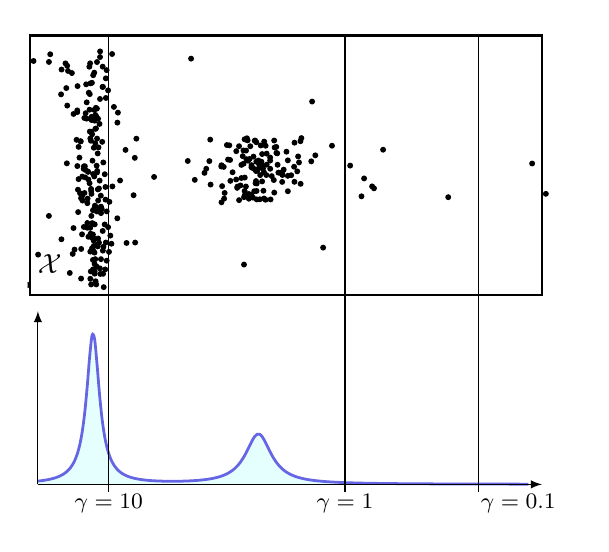
\begin{tikzpicture}[scale=1,declare function={%
    %%cauchy distrib
    c1 = 6.0/10.0;
    c2 = 4.0/10.0;
    seuil = c1/(c1+c2);
    a1 = 0.1;
    a2 = 0.2;
    x01 = 0.8;
    x02 = 2.9;
    cauchyMass1(\x) = c1*a1/( pi*( pow(a1,2) + pow((\x-x01),2) ));
    cauchyMass2(\x) = c2*a2/( pi*( pow(a2,2) + pow((\x-x02),2) ));
      cauchyRepFuncInv1(\x) = a1*tan( 3.142*(\x-0.5) r) + x01;
      cauchyRepFuncInv2(\x) = a2*tan( 3.142*(\x-0.5) r) + x02;
      indicatorFunction(\x) = exp(-pow(\x-3,2)/6);
      %%params
      firstVerticalSplitX = 1;
      lastVerticalSplitX = 5.7;
      verticalDashedSplitX = 2.3;
      verticalSplitX = 4;
      lowHorizontalDashedSplitY = 4.5;
      highHorizontalDashedSplitY = 5.5;
      coeffHomothety = 3.8;
      homothetyBone = -1.7;
      homothetyBtwo = -14;
    },
]
    \definecolor{niceblue}{rgb}{0.4,0.4,0.9}
    \definecolor{blue2}{rgb}{0.9,1,1}

    %%% draw area
    \clip (-0.03,0.5) rectangle (7,6.8);

    %%% TOP RECTANGLES
    \draw[thick] (0,3.4) rectangle (6.5,6.7);
    %\draw[thick] (7,3.4) rectangle (13.5,6.7);
    \node at (0.25,3.8) {$\mathcal{X}$};
    %\node at (7.25,3.8) {$\mathcal{X}_t$};
    %\node[color=niceblue] at
    %(verticalSplitX+0.3,lowHorizontalDashedSplitY-0.2) {$\mathcal{X}_t$};


    %%%%%%%%%%%%%%%%%% LEFT PART
    %%% points sampling
    \foreach \x in {1,2,...,350}{
    \pgfmathsetmacro{\seuil}{c1/(c1+c2)}
    \pgfmathsetmacro{\aleatorio}{rnd}
    \pgfmathsetmacro{\rndCauchy}{\aleatorio>seuil ? 0 : 1 }
    \pgfmathsetmacro{\abscissePoint}{\rndCauchy*cauchyRepFuncInv1(rand) +
    (1-\rndCauchy)*cauchyRepFuncInv2(rand)}
    \pgfmathsetmacro{\ordinatePoint}{\rndCauchy*(1.5*rand+5) +
    (1-\rndCauchy)*(rand*0.4+5)}
    \pgfmathsetmacro{\abscissePointFiltered}{ \abscissePoint>6.6 ? -10 :
    \abscissePoint }
    \pointSampled{\abscissePointFiltered,\ordinatePoint}
    %\pgfmathsetmacro{\rightEnough}{\abscissePoint>verticalDashedSplitX ? true
    %: false }
    %\pgfmathsetmacro{\leftEnough}{\abscissePoint<verticalSplitX ? true : false
    %}
    %\pgfmathsetmacro{\highEnough}{\ordinatePoint>lowHorizontalDashedSplitY ?
    %true : false}
    %\pgfmathsetmacro{\lowEnough}{\ordinatePoint<highHorizontalDashedSplitY ?
    %true : false}
    %\pgfmathsetmacro{\newAbscisse}{\rightEnough && \leftEnough && \highEnough
    %&& \lowEnough ? \abscissePoint*coeffHomothety + homothetyBone : -10  }
    %\pointSampled{\newAbscisse,\ordinatePoint*coeffHomothety + homothetyBtwo}
  }


  %% curve
 \fill [blue2, domain=0.1:6.33, variable=\x]
      (0.1, 1)
      -- plot[samples=200,smooth] ({\x},{cauchyMass1(\x) + cauchyMass2(\x) +1}
      )
      -- (6.33, 1)
      -- cycle;
  \draw [domain=0.1:6.33, scale=1, color=niceblue, line width=1pt, fill=blue2]
  plot[samples=200,smooth] (\x,{cauchyMass1(\x) + cauchyMass2(\x) +1});
  %% axis
  \draw[->,>=latex] (0.1,1) to (0.1,3.2);
  \draw[->,>=latex] (0.1,1) to (6.5,1);

  %% splits
  \draw (firstVerticalSplitX,0.9) -- (firstVerticalSplitX,6.7); % gamma=10
  \draw (verticalSplitX,0.9) -- (verticalSplitX,6.7); % gamma=1
  \draw (lastVerticalSplitX,0.9) -- (lastVerticalSplitX,6.7); % gamma=0.1
  \node[below] at (firstVerticalSplitX,1){\footnotesize $\gamma=10$};
  \node[below] at (verticalSplitX,1){\footnotesize $\gamma=1$};
  \node[below] at (lastVerticalSplitX+0.5,1){\footnotesize $\gamma=0.1$};
  %\draw (verticalDashedSplitX,0.9) -- (verticalDashedSplitX,6.7);
  %\draw (0,lowHorizontalDashedSplitY) -- (6.5,lowHorizontalDashedSplitY);
  %\draw (0,highHorizontalDashedSplitY) -- (6.5,highHorizontalDashedSplitY);
  %% ZOOM
  %\draw[very thick, color=niceblue]
  %(verticalDashedSplitX,lowHorizontalDashedSplitY) rectangle
  %(verticalSplitX,highHorizontalDashedSplitY);
  %\draw[very thick, dashed, color=niceblue,->,>=latex]
  %(verticalDashedSplitX,highHorizontalDashedSplitY) -- (7,6.7);
  %\draw[very thick, dashed, color=niceblue,->,>=latex]
  %(verticalDashedSplitX,lowHorizontalDashedSplitY) -- (7,3.4);

  %%%%%%%%%%%%%%%%%% RIGHT PART second curve
  \vide{
  \fill [blue2, domain=7.1:13.53, variable=\x]
      (7.1, 1)
      -- plot[samples=200,smooth] ({\x},{
      indicatorFunction((\x-7)/5)*coeffHomothety*1.5*cauchyMass2((\x -
      homothetyBone)/coeffHomothety)
      +1 } )
      -- (13.53, 1)
      -- cycle;
  \draw[->,>=latex] (7.1,1) to (7.1,3.2);
  \draw[->,>=latex] (7.1,1) to (13.7,1);
  \draw [domain=7.1:13.53, scale=1, color=niceblue, line width=1pt]
  plot[samples=200,smooth] (\x,{
  indicatorFunction((\x-7)/5)*1.5*coeffHomothety*cauchyMass2((\x -
  homothetyBone)/coeffHomothety)
  +1} );

  %% splits
  \draw (verticalSplitX+7.25,0.9) -- (verticalSplitX+7.25,6.7); % gamma=1
  \draw (13.36,0.9) -- (13.36,6.7); % gammat
  \node[below] (gammaone) at (verticalSplitX+7.25,1){\footnotesize $\gamma=1$};
  \node[below] (gammat) at (13.36,1){\footnotesize $\gamma_t$};
  \draw[dashed] (7.1,1.23) -- (verticalSplitX+7.25,1.23);
  \node[right] at (6.65,1.35){\footnotesize $t_{\gamma}$};

  \draw[->,>=latex, very thick, color=niceblue] (13.3,1.3) to[bend right]
  (verticalSplitX+7.3,1.3);
  \node at (verticalSplitX+8.2,2)  {\color{niceblue} \textbf{adaptivity}};
  }
\end{tikzpicture}}

\caption{Illustration of the standard splitting
criterion on two modes when the proportion $\gamma$ varies.
\label{ocrf:fig:split_alpha_2}}
\end{figure}
\section{Hyper-parameters of tested algorithms}
\label{supp:hyper_choice}
Overall we chose to train the different algorithms with their (default)
hyper-parameters as seen in their respective paper or author's implementation.
Indeed, since we are in an unsupervised setting, there is no trivial way to
select/learn the hyperparameters of the different algorithm in the training
phase -- the labels are not supposed to be available. Hence the more realistic
way to test the algorithms is to use their recommended/default hyperparameters.
\paragraph{}
The \ac{OCSVM} algorithm uses default parameters: \texttt{kernel='rbf'} with
\texttt{tol=1e-3}, \texttt{nu=0.5}, \texttt{shrinking=True} and
\texttt{gamma=1/n\textunderscore features}, where tol is the tolerance for
stopping
criterion.
\paragraph{}
The \ac{LOF} algorithm uses default parameters: \texttt{n\textunderscore
neighbors=5} with the \texttt{leaf\textunderscore size=30} and
\texttt{metric='minkowski'} and \texttt{contamination=0.1} and
\texttt{algorithm='auto'}, where the algorithm parameters stipulates how to
compute the nearest neighbors (either ball-tree, kd-tree or brute-force).
\paragraph{}
The \ac{iForest} algorithm uses default parameters: \texttt{n\textunderscore
estimators=100} and \texttt{max\textunderscore samples=min(256, n\textunderscore
samples)} and \texttt{max\textunderscore features=1} and setting
\texttt{bootstrap=false}, where bootstrap states whether samples are drawn with
replacement.
\paragraph{}
The \acs{OCRFsampling} algorithm uses default parameters: the number of
dimensions for the Random Subspace Method \texttt{krsm=-1}, the number of
features randomly selected at each node during the induction of the tree
\texttt{krfs=-1}, \texttt{n\textunderscore tree=100}, the factor controlling
the extension of the outlier domain used to sample outliers according to the
volume of the hyper-box surrounding the target data \texttt{alpha=1.2}, the
factor controlling the number of outlier data generated according to the number
of target data \texttt{beta=10}, whether outliers are generated from uniform
distribution \texttt{optimize=0} and eventually whether data outside target
bounds are considered as outlier data \texttt{rejectOutOfBounds=0}.
\paragraph{}
The \emph{Orca} algorithm uses default parameter \texttt{k=5} (number of
nearest neighbors) as well as \texttt{N=n/8} (how many anomalies are to be
reported).  The last setting, set up in the empirical evaluation of iForest in
\citet{Liu2012}, allows a better computation time without impacting Orca's
performance.
\paragraph{}
The \ac{RFC} algorithm uses default parameters: \texttt{no.forests=25} with the
number of trees \texttt{no.trees=3000}, the Addcl1 Random Forest dissimilarity
\texttt{addcl1=T}, \texttt{addcl2=F} use the importance measure \texttt{imp=T},
the data generating process \texttt{oob.prox1=T}, the number of features
sampled at each split \texttt{mtry1=3}.
\paragraph{}
The \ac{LSAD} algorithm uses default parameters: the maximum number of samples
per kernel \texttt{n\textunderscore kernels\textunderscore max=500}, the center
of each kernel (the center of the random sample subset by default)
\texttt{kernel\textunderscore pos='None'}, the kernel scale parameter (using
the pairwise median trick by default \citep{jaakkola1999using})
\texttt{gamma='None'}, the regularization parameter \texttt{rho=0.1}.

\section{Description of the datasets}
\label{supp:dataset_description}
%
The characteristics of the twelve reference datasets considered here are
summarized in \cref{ocrf:table:data}. They are all available on the \acs{UCI}
repository \citep{Lichman2013} and the preprocessing is done in a classical
way.
%, excepting for the \emph{adult} dataset. For the latter, we considered the 6
%continuous features.
In anomaly detection, we typically have data from two class (inliers/outliers)
-- in novelty detection, the second class is unavailable in training in outlier
detection, training data are polluted by second class (anonymous) examples. The
classical approach to adapt multi-class data to this framework is to set
classes forming the outlier class, while the other classes form the inlier
class.
\paragraph{}
We removed all categorial attributes. Indeed, our method is designed to handle
data whose distribution is absolutely continuous \acs{wrt}~the Lebesgue
measure.
% If this is not the case but there is still a suffiently large number of
% different values (say, greater than 10), it is still worth testing our method
% with this kind of data.
%
The \emph{http} and \emph{smtp} datasets belong to the \acs{KDD} Cup '99
dataset \citep{KDD99, Tavallaee2009}, which consist of a wide variety of
hand-injected attacks (anomalies) in a closed network (normal/inlier
background). They are classically obtained as described in
\citet{Yamanishi2000}. This two datasets are available on the
\emph{scikit-learn} library \citep{pedregosa2011scikit}. The \emph{shuttle}
dataset is the fusion of the training and testing datasets available in the
\acs{UCI} repository. As in \citet{Liu2008}, we use instances from all
different classes but class $4$.
%, which yields an anomaly ratio (class 1) of $7.17\%$.
In the \emph{forestcover} data, the inliers are the instances from class~$2$
while instances from class $4$ are anomalies (as in \citet{Liu2008}).
%, which yields an anomaly ratio of $0.9\%$.
The \emph{ionosphere} dataset differentiates \say{good} from \say{bad} radars,
considered here as abnormal. A \say{good} radar shows evidence of some type of
structure in the ionosphere. A \say{bad} radar does not, its signal passing
through the ionosphere.
The \emph{spambase} dataset consists of spam or non-spam emails. The former
constitute our anomaly class.  The \emph{annthyroid} medical dataset on
hypothyroidism contains one normal class and two abnormal ones, which form our
outliers.
The \emph{arrhythmia} dataset reflects the presence and absence (class $1$) of
cardiac arrhythmia. The number of attributes being large considering the sample
size, we removed attributes containing missing data.  Besides, we removed
attributes taking less than $10$ different values, the latter breaking too
strongly our absolutely continuous assumption (\acs{wrt}~to $\Leb$).
The \emph{pendigits} dataset contains 10 classes corresponding to the digits
from 0 to 9, examples being handwriting samples. As in \citet{Schubert2012},
the outliers are chosen to be those from class 4.  The \emph{pima} dataset
consists of medical data on diabetes. Patients suffering from diabetes (inlier
class) were considered outliers.  The \emph{wild} dataset involves detecting
diseased trees in Quickbird imagery. Diseased trees (class `w') is our outlier
class.  In the \emph{adult} dataset, the goal is to predict whether income
exceeds \$ 50K/year based on census data. We only keep the 6 continuous
attributes.
\pgfplotsset{minor grid style={very thick,black}}
\begin{figure}
    \centering
    \definecolor{ggreen}{rgb}{0.3,0.7,0.4}
    \definecolor{ggreen2}{rgb}{0.4,0.8,0.5}
    \definecolor{orange2}{rgb}{1,0.7,0}
    \definecolor{violette}{rgb}{0.7,0.15,0.9}
    \resizebox{\textwidth}{!}{%
    \begin{tikzpicture}[scale=0.6,font=\Large]
        \begin{axis}[ at={(0,0)},
                      grid=minor,
                      width=23cm, height=6cm,
                      ybar=0pt,
                      minor xtick={0.5,1.5,...,12.5},
                      xmin=0.5, xmax=12.5,
                      xticklabels={ , , , , , , , , , , , },
                      ymin=0.58,
                      ytick={0.6,0.7,...,1},
                      ymax=1,
                      ylabel={\acs{ROC} \acs{AUC}}, legend
                      entries={\acs{OneClassRF}~~~~,\acs{iForest}~~~~,
                      \acs{OCRFsampling}~~~~, \acs{OCSVM}~~~~, \acs{LOF}~~~~,
                      Orca~~~~, \acs{LSAD}~~~~, \acs{RFC}},
                      legend style={at={(0.5,1.16)}, anchor=north,legend
                      columns=-1}
                      ]
        \draw[dashed,black!30] (axis cs:0,0.6)--(axis cs:12.5,0.6);
        \draw[dashed,black!30] (axis cs:0,0.7)--(axis cs:12.5,0.7);
        \draw[dashed,black!30] (axis cs:0,0.8)--(axis cs:12.5,0.8);
        \draw[dashed,black!30] (axis cs:0,0.9)--(axis cs:12.5,0.9);
        \addplot+[bar width=4.5pt] plot table[x index=1, y
        index=3]{./resultsOCRF/results_semisupervised.txt};%OneClassRF
        \addplot+[bar width=4.5pt] plot table[x index=1, y
        index=7]{./resultsOCRF/results_semisupervised.txt};%iForest
        \addplot+[bar width=4.5pt] plot table[x index=1, y
        index=11]{./resultsOCRF/results_semisupervised.txt};%OCRFsampling
        \addplot+[bar width=4.5pt] plot table[x index=1, y
        index=15]{./resultsOCRF/results_semisupervised.txt};%OneClassSVM
        \addplot+[bar width=4.5pt, fill=ggreen!50, draw=ggreen] plot table[x
        index=1, y index=19]{./resultsOCRF/results_semisupervised.txt};%LOF
        \addplot+[bar width=4.5pt, fill=violette!50, draw=violette] plot
        table[x index=1, y
        index=23]{./resultsOCRF/results_semisupervised.txt};%ORCA
        \addplot+[bar width=4.5pt, fill=orange2!50, draw=orange2] plot table[x
        index=1, y index=27]{./resultsOCRF/results_semisupervised.txt};%LSAD
        \addplot+[bar width=4.5pt,fill=white, draw=black!40] plot table[x
        index=1, y index=31]{../resultsOCRF/results_semisupervised.txt};%RFC
        \end{axis}
        \begin{axis}[ at={(0,-5cm)},
                      grid=minor,
                      width=23cm, height=6cm,
                      ybar=0pt,
                      minor xtick={0.5,1.5,...,12.5},
                      xmin=0.5, xmax=12.5,
                      xticklabels={ , , , , , , , , , , , },
                      ymin=0.0,
                      ytick={0.2,0.4,0.6,0.8,1},
                      ymax=1,
                      ylabel={\acs{PR} \acs{AUC}},
                      %legend entries={OneClassRF~~~~,iForest~~~~,
                      %OCRFsampling~~~~, OneClassSVM~~~~, LOF~~~~, Orca~~~~,
                      %LSAD~~~~, RFC},
                      legend style={at={(0.5,1.16)}, anchor=north,legend
                      columns=-1}
                      ]
        \draw[dashed,black!30] (axis cs:0,0.2)--(axis cs:12.5,0.2);
        \draw[dashed,black!30] (axis cs:0,0.4)--(axis cs:12.5,0.4);
        \draw[dashed,black!30] (axis cs:0,0.6)--(axis cs:12.5,0.6);
        \draw[dashed,black!30] (axis cs:0,0.8)--(axis cs:12.5,0.8);
        \addplot+[bar width=4.5pt] plot table[x index=1, y
        index=5]{./resultsOCRF/results_semisupervised.txt};%OneClassRF
        \addplot+[bar width=4.5pt] plot table[x index=1, y
        index=9]{./resultsOCRF/results_semisupervised.txt};%iForest
        \addplot+[bar width=4.5pt] plot table[x index=1, y
        index=13]{./resultsOCRF/results_semisupervised.txt};%OCRFsampling
        \addplot+[bar width=4.5pt] plot table[x index=1, y
        index=17]{./resultsOCRF/results_semisupervised.txt};%OneClassSVM
        \addplot+[bar width=4.5pt, fill=ggreen!50, draw=ggreen] plot table[x
        index=1, y index=21]{./resultsOCRF/results_semisupervised.txt};%LOF
        \addplot+[bar width=4.5pt, fill=violette!50, draw=violette] plot
        table[x index=1, y
        index=25]{./resultsOCRF/results_unsupervised.txt};%ORCA
        \addplot+[bar width=4.5pt, fill=orange2!50, draw=orange2] plot table[x
        index=1, y index=29]{./resultsOCRF/results_semisupervised.txt};%LSAD
        \addplot+[bar width=4.5pt,fill=white, draw=black!40] plot table[x
        index=1, y index=33]{./resultsOCRF/results_semisupervised.txt};%RFC
        \end{axis}
        \begin{axis}[  at={(0,-13.4)},
                      grid=minor,
                      width=23cm,height=6cm,
                      ybar=0pt,
                      minor xtick={0.5,1.5,...,12.5},
                      xmin=0.5, xmax=12.5,
                      xtick={1,...,12},
                      xticklabels={adult, annthyroid, arrhythmia, forestcover,
                      http, ionosphere, pendigits, pima, shuttle, smtp,
                      spambase, wilt},
                      x tick label style={rotate=20,anchor=east},
                      ymax=60, ymin=0,
                      ytick={0,10,...,60},
                      ylabel={Computation time (sec.)}
                      ]
        \draw[dashed,black!30] (axis cs:0,10)--(axis cs:12.5,10);
        \draw[dashed,black!30] (axis cs:0,20)--(axis cs:12.5,20);
        \draw[dashed,black!30] (axis cs:0,30)--(axis cs:12.5,30);
        \draw[dashed,black!30] (axis cs:0,40)--(axis cs:12.5,40);
        \draw[dashed,black!30] (axis cs:0,50)--(axis cs:12.5,50);
        \addplot+[bar width=4.5pt] plot table[x index=1, y
        index=2]{./resultsOCRF/computationTime_semisupervised.txt};%OneClassRF
        \addplot+[bar width=4.5pt] plot table[x index=1, y
        index=5]{./resultsOCRF/computationTime_semisupervised.txt};%iForest
        \addplot+[bar width=4.5pt] plot table[x index=1, y
        index=8]{./resultsOCRF/computationTime_semisupervised.txt};%OCRFsampling
        \addplot+[bar width=4.5pt] plot table[x index=1, y
        index=9]{./resultsOCRF/computationTime_semisupervised.txt};%OneClassSVM
        \addplot+[bar width=4.5pt, fill=ggreen!50, draw=ggreen] plot table[x
        index=1, y
        index=12]{./resultsOCRF/computationTime_semisupervised.txt};%LOF
        \addplot+[bar width=4.5pt, fill=violette!50, draw=violette] plot
        table[x index=1, y
        index=15]{./resultsOCRF/computationTime_semisupervised.txt};%ORCA
        \addplot+[bar width=4.5pt, fill=orange2!50, draw=orange2] plot table[x
        index=1, y
        index=16]{./resultsOCRF/computationTime_semisupervised.txt};%LSAD
        \addplot+[bar width=4.5pt,fill=white, draw=black!40] plot table[x
        index=1, y
        index=19]{./resultsOCRF/computationTime_semisupervised.txt};%RFC
        \end{axis}
    \end{tikzpicture}}
    \caption[Performances of the novelety detection algorithms]{Performances of
    the algorithms on each dataset in the novelty detection framework:
    \acs{ROC} \acsp{AUC} are displayed on the top, \acs{PR} \acsp{AUC} in the
    middle and training times on the bottom, for each dataset and algorithm.
    The $x$-axis represents the datasets.
    \label{ocrf:figresultssemisupervised}}
\end{figure}
\pgfplotsset{minor grid style={very thick,black}}
\begin{figure}
    \centering
    \definecolor{ggreen}{rgb}{0.3,0.7,0.4}
    \definecolor{ggreen2}{rgb}{0.4,0.8,0.5}
    \definecolor{orange2}{rgb}{1,0.7,0}
    \definecolor{violette}{rgb}{0.7,0.15,0.9}
    \resizebox{\textwidth}{!}{%
    \begin{tikzpicture}[scale=0.6,font=\Large]
        \begin{axis}[ at={(0,0)},
                      grid=minor,
                      width=23cm, height=6cm,
                      ybar=0pt,
                      minor xtick={0.5,1.5,...,12.5},
                      xmin=0.5, xmax=12.5,
                      xticklabels={ , , , , , , , , , , , },
                      ymin=0.45,
                      ytick={0.5,0.6,0.7,...,1},
                      ymax=1,
                      ylabel={\acs{ROC} \acs{AUC}},
                      legend entries={\acs{OneClassRF}~~~~,\acs{iForest}~~~~,
                      \acs{OCRFsampling}~~~~, \acs{OCSVM}~~~~, \acs{LOF}~~~~,
                      Orca~~~~, \acs{LSAD}~~~~, \acs{RFC}},
                      legend style={at={(0.5,1.16)}, anchor=north,legend
                      columns=-1}
                      ]
            \draw[dashed,black!30] (axis cs:0,0.6)--(axis cs:12.5,0.6);
            \draw[dashed,black!30] (axis cs:0,0.7)--(axis cs:12.5,0.7);
            \draw[dashed,black!30] (axis cs:0,0.8)--(axis cs:12.5,0.8);
            \draw[dashed,black!30] (axis cs:0,0.9)--(axis cs:12.5,0.9);
            \addplot+[bar width=4.5pt] plot table[x index=1, y
            index=3]{./resultsOCRF/results_unsupervised.txt};%OneClassRF
            \addplot+[bar width=4.5pt] plot table[x index=1, y
            index=7]{./resultsOCRF/results_unsupervised.txt};%iForest
            \addplot+[bar width=4.5pt] plot table[x index=1, y
            index=11]{./resultsOCRF/results_unsupervised.txt};%OCRFsampling
            \addplot+[bar width=4.5pt] plot table[x index=1, y
            index=15]{./resultsOCRF/results_unsupervised.txt};%OneClassSVM
            \addplot+[bar width=4.5pt, fill=ggreen!50, draw=ggreen] plot
            table[x index=1, y
            index=19]{./resultsOCRF/results_unsupervised.txt};%LOF
            \addplot+[bar width=4.5pt, fill=violette!50, draw=violette] plot
            table[x index=1, y
            index=23]{./resultsOCRF/results_unsupervised.txt};%ORCA
            \addplot+[bar width=4.5pt, fill=orange2!50, draw=orange2] plot
            table[x index=1, y
            index=27]{./resultsOCRF/results_unsupervised.txt};%LSAD
            \addplot+[bar width=4.5pt,fill=white, draw=black!40] plot table[x
            index=1, y index=31]{../resultsOCRF/results_unsupervised.txt};%RFC
        \end{axis}

        \begin{axis}[  at={(0,-5cm)},
                      grid=minor,
                      width=23cm,height=6cm,
                      ybar=0pt,
                      minor xtick={0.5,1.5,...,12.5},
                      xmin=0.5, xmax=12.5,
                      xtick={1,...,12},
                      xticklabels={ , , , , , , , , , , , },
                      x tick label style={rotate=20,anchor=east},
                      ytick={0.2,0.4,0.6,0.8,1},
                      ymin=0,
                      ymax=1,
                      ylabel={\acs{PR} \acs{AUC}}
                      ]
            %\draw[dashed,black!30] (axis cs:0,10)--(axis cs:12.5,10);
            %\draw[dashed,black!30] (axis cs:0,20)--(axis cs:12.5,20);
            %\draw[dashed,black!30] (axis cs:0,30)--(axis cs:12.5,30);
            %\draw[dashed,black!30] (axis cs:0,40)--(axis cs:12.5,40);
            %\draw[dashed,black!30] (axis cs:0,50)--(axis cs:12.5,50);
            \draw[dashed,black!30] (axis cs:0,0.2)--(axis cs:12.5,0.2);
            \draw[dashed,black!30] (axis cs:0,0.4)--(axis cs:12.5,0.4);
            \draw[dashed,black!30] (axis cs:0,0.6)--(axis cs:12.5,0.6);
            \draw[dashed,black!30] (axis cs:0,0.8)--(axis cs:12.5,0.8);
            \addplot+[bar width=4.5pt] plot table[x index=1, y
            index=5]{./resultsOCRF/results_unsupervised.txt};%OneClassRF
            \addplot+[bar width=4.5pt] plot table[x index=1, y
            index=9]{./resultsOCRF/results_unsupervised.txt};%iForest
            \addplot+[bar width=4.5pt] plot table[x index=1, y
            index=13]{./resultsOCRF/results_unsupervised.txt};%OCRFsampling
            \addplot+[bar width=4.5pt] plot table[x index=1, y
            index=17]{./resultsOCRF/results_unsupervised.txt};%OneClassSVM
            \addplot+[bar width=4.5pt, fill=ggreen!50, draw=ggreen] plot
            table[x index=1, y
            index=21]{./resultsOCRF/results_unsupervised.txt};%LOF
            \addplot+[bar width=4.5pt, fill=violette!50, draw=violette] plot
            table[x index=1, y
            index=25]{./resultsOCRF/results_unsupervised.txt};%ORCA
            \addplot+[bar width=4.5pt, fill=orange2!50, draw=orange2] plot
            table[x index=1, y
            index=29]{./resultsOCRF/results_unsupervised.txt};%LSAD
            \addplot+[bar width=4.5pt,fill=white, draw=black!40] plot table[x
            index=1, y index=33]{./resultsOCRF/results_unsupervised.txt};%RFC
        \end{axis}

        \begin{axis}[  at={(0,-13.4)},
                      grid=minor,
                      width=23cm,height=6cm,
                      ybar=0pt,
                      minor xtick={0.5,1.5,...,12.5},
                      xmin=0.5, xmax=12.5,
                      xtick={1,...,12},
                      xticklabels={adult, annthyroid, arrhythmia, forestcover,
                      http, ionosphere, pendigits, pima, shuttle, smtp,
                      spambase, wilt},
                      x tick label style={rotate=20,anchor=east},
                      ymax=60, ymin=0,
                      ytick={0,10,...,60},
                      ylabel={Computation time (sec.)}
                      ]
        \draw[dashed,black!30] (axis cs:0,10)--(axis cs:12.5,10);
        \draw[dashed,black!30] (axis cs:0,20)--(axis cs:12.5,20);
        \draw[dashed,black!30] (axis cs:0,30)--(axis cs:12.5,30);
        \draw[dashed,black!30] (axis cs:0,40)--(axis cs:12.5,40);
        \draw[dashed,black!30] (axis cs:0,50)--(axis cs:12.5,50);
        \addplot+[bar width=4.5pt] plot table[x index=1, y
        index=2]{./resultsOCRF/computationTime_unsupervised.txt};%OneClassRF
        \addplot+[bar width=4.5pt] plot table[x index=1, y
        index=5]{./resultsOCRF/computationTime_unsupervised.txt};%iForest
        \addplot+[bar width=4.5pt] plot table[x index=1, y
        index=8]{./resultsOCRF/computationTime_unsupervised.txt};%OCRFsampling
        \addplot+[bar width=4.5pt] plot table[x index=1, y
        index=9]{./resultsOCRF/computationTime_unsupervised.txt};%OneClassSVM
        \addplot+[bar width=4.5pt, fill=ggreen!50, draw=ggreen] plot table[x
        index=1, y
        index=12]{./resultsOCRF/computationTime_unsupervised.txt};%LOF
        \addplot+[bar width=4.5pt, fill=violette!50, draw=violette] plot
        table[x index=1, y
        index=15]{./resultsOCRF/computationTime_unsupervised.txt};%ORCA
        \addplot+[bar width=4.5pt, fill=orange2!50, draw=orange2] plot table[x
        index=1, y
        index=16]{./resultsOCRF/computationTime_unsupervised.txt};%LSAD
        \addplot+[bar width=4.5pt,fill=white, draw=black!40] plot table[x
        index=1, y
        index=19]{./resultsOCRF/computationTime_unsupervised.txt};%RFC
        \end{axis}
    \end{tikzpicture}}
    \caption[Performances of the outlier detection algorithms]{Performances of
    the algorithms on each dataset in the outlier detection framework:
    \acs{ROC} \acsp{AUC} are on the top, \acs{PR} \acsp{AUC} in the middle and
    processing times are displayed below (for each dataset and algorithm). The
    $x$-axis represents the datasets.  \label{ocrf:figresultsunsupervised}}
\end{figure}
%Concerning the \emph{internet_ads} dataset, it contains characteristic of
%images, which may (class `ad', outlier) or not (class `nonad') be an
%advertisement.
\section{Further details on benchmarks and outlier detection results}
\label{sup:outlier_detection}


\Cref{ocrf:figresultssemisupervised} shows that the amount of time to
train\footnote{For \ac{OneClassRF}, Orca and \ac{RFC}, testing and training
time cannot be isolated because of algorithms implementation: for these
algorithms, the sum of the training and testing times are displayed in
\Cref{ocrf:figresultssemisupervised} and \Cref{ocrf:figresultsunsupervised}.}
and test any dataset takes less than one minute with \ac{OneClassRF}, whereas
some algorithms have far higher computation times (\ac{OCRFsampling},
\ac{OCSVM}, \ac{LOF} and Orca have computation times higher than $30$ minutes
in some datasets). Our approach yields results similar to quite new algorithms
such as \ac{iForest} and \ac{LSAD}.
We also present experiments in the outlier detections setting. For each
algorithm, $10$ experiments on random training and testing datasets are
performed. Averaged \acs{ROC} and \acs{PR} curves \acs{AUC} are summarized in
\cref{ocrf:table:results-unsupervised}.
%
For the experiments made in an unsupervised framework (meaning that the
training set is polluted by outliers), the anomaly rate is arbitrarily bounded
to $10\%$ max (before splitting data into training and testing sets).
%XXX TODO: description of the table
% M = np.array([[ 0.625, 0.161, 0.644, 0.234, np.NAN, np.NAN, 0.622, 0.179,
% 0.546 , 0.100   , 0.593 , 0.179   , 0.633 , 0.204       , np.NAN   , np.NAN],
% [ 0.842 , 0.226   , 0.820 , 0.310   , 0.992 , 0.869   , 0.688 , 0.193   ,
% 0.731 , 0.188   , 0.561 , 0.132   , 0.762 , 0.246       , np.NAN   , np.NAN],
% [ 0.698 , 0.485   , 0.746 , 0.418   , 0.704 , 0.276   , 0.916 , 0.630   ,
% 0.765 , 0.468   , 0.741 , 0.502   , 0.733 , 0.393       , 0.711 , 0.309], [
% 0.845 , 0.044   , 0.882 , 0.062   , np.NAN   , np.NAN     , np.NAN , np.NAN
% , 0.550 , 0.017   , 0.696 , 0.045   , 0.816 , 0.072       , np.NAN   ,
% np.NAN], [ 0.984 , 0.120   , 0.999 , 0.685   , np.NAN   , np.NAN    , np.NAN
% , np.NAN   , np.NAN   , np.NAN     , 0.998 , 0.402   , 0.277 , 0.074       ,
% np.NAN   , np.NAN], [ 0.903 , 0.508   , 0.888 , 0.545   , 0.879 , 0.664   ,
% 0.956 , 0.813   , 0.956 , 0.789   , 0.929 , 0.917   , 0.915 , 0.773       ,
% 0.943 , 0.725], [ 0.453 , 0.085   , 0.463 , 0.077   , 0.999 , 0.993   , 0.366
% , 0.066   , 0.491 , 0.086   , 0.495 , 0.086   , 0.513 , 0.091       , np.NAN
% , np.NAN], [ 0.708 , 0.229   , 0.743 , 0.205   , 0.790 , 0.296   , 0.706 ,
% 0.226   , 0.670 , 0.137   , 0.585 , 0.170   , 0.686 , 0.190       , 0.505 ,
% 0.091], [ 0.947 , 0.491   , 0.997 , 0.979   , np.NAN   , np.NAN     , 0.992 ,
% 0.904   , 0.526 , 0.115   , 0.655 , 0.320   , 0.686 , 0.218       , np.NAN  ,
% np.NAN], [ 0.916 , 0.400   , 0.902 , 0.005   , np.NAN   , np.NAN     , 0.881
% , 0.372   , 0.909 , 0.053   , 0.824 , 0.236   , 0.888 , 0.398       , np.NAN
% , np.NAN], [ 0.830 , 0.300   , 0.799 , 0.303   , 0.970 , 0.877   , 0.722 ,
% 0.192   , 0.664 , 0.120   , 0.603 , 0.210   , 0.731 , 0.229       , 0.684 ,
% 0.134], [ 0.520 , 0.053   , 0.443 , 0.044   , 0.966 , 0.554   , 0.316 , 0.036
% , 0.627 , 0.069   , 0.441 , 0.029   , 0.530 , 0.053       , 0.876 , 0.472]])
% np.nanmean(M, axis=0)


\begin{figure*}[!ht]
    \caption{\acs{ROC} and \acs{PR} curves for \acs{OneClassRF} (novelty
    detection framework)}
    \label{ocrf:fig:oneclassrf_roc_pr}
    \centering
    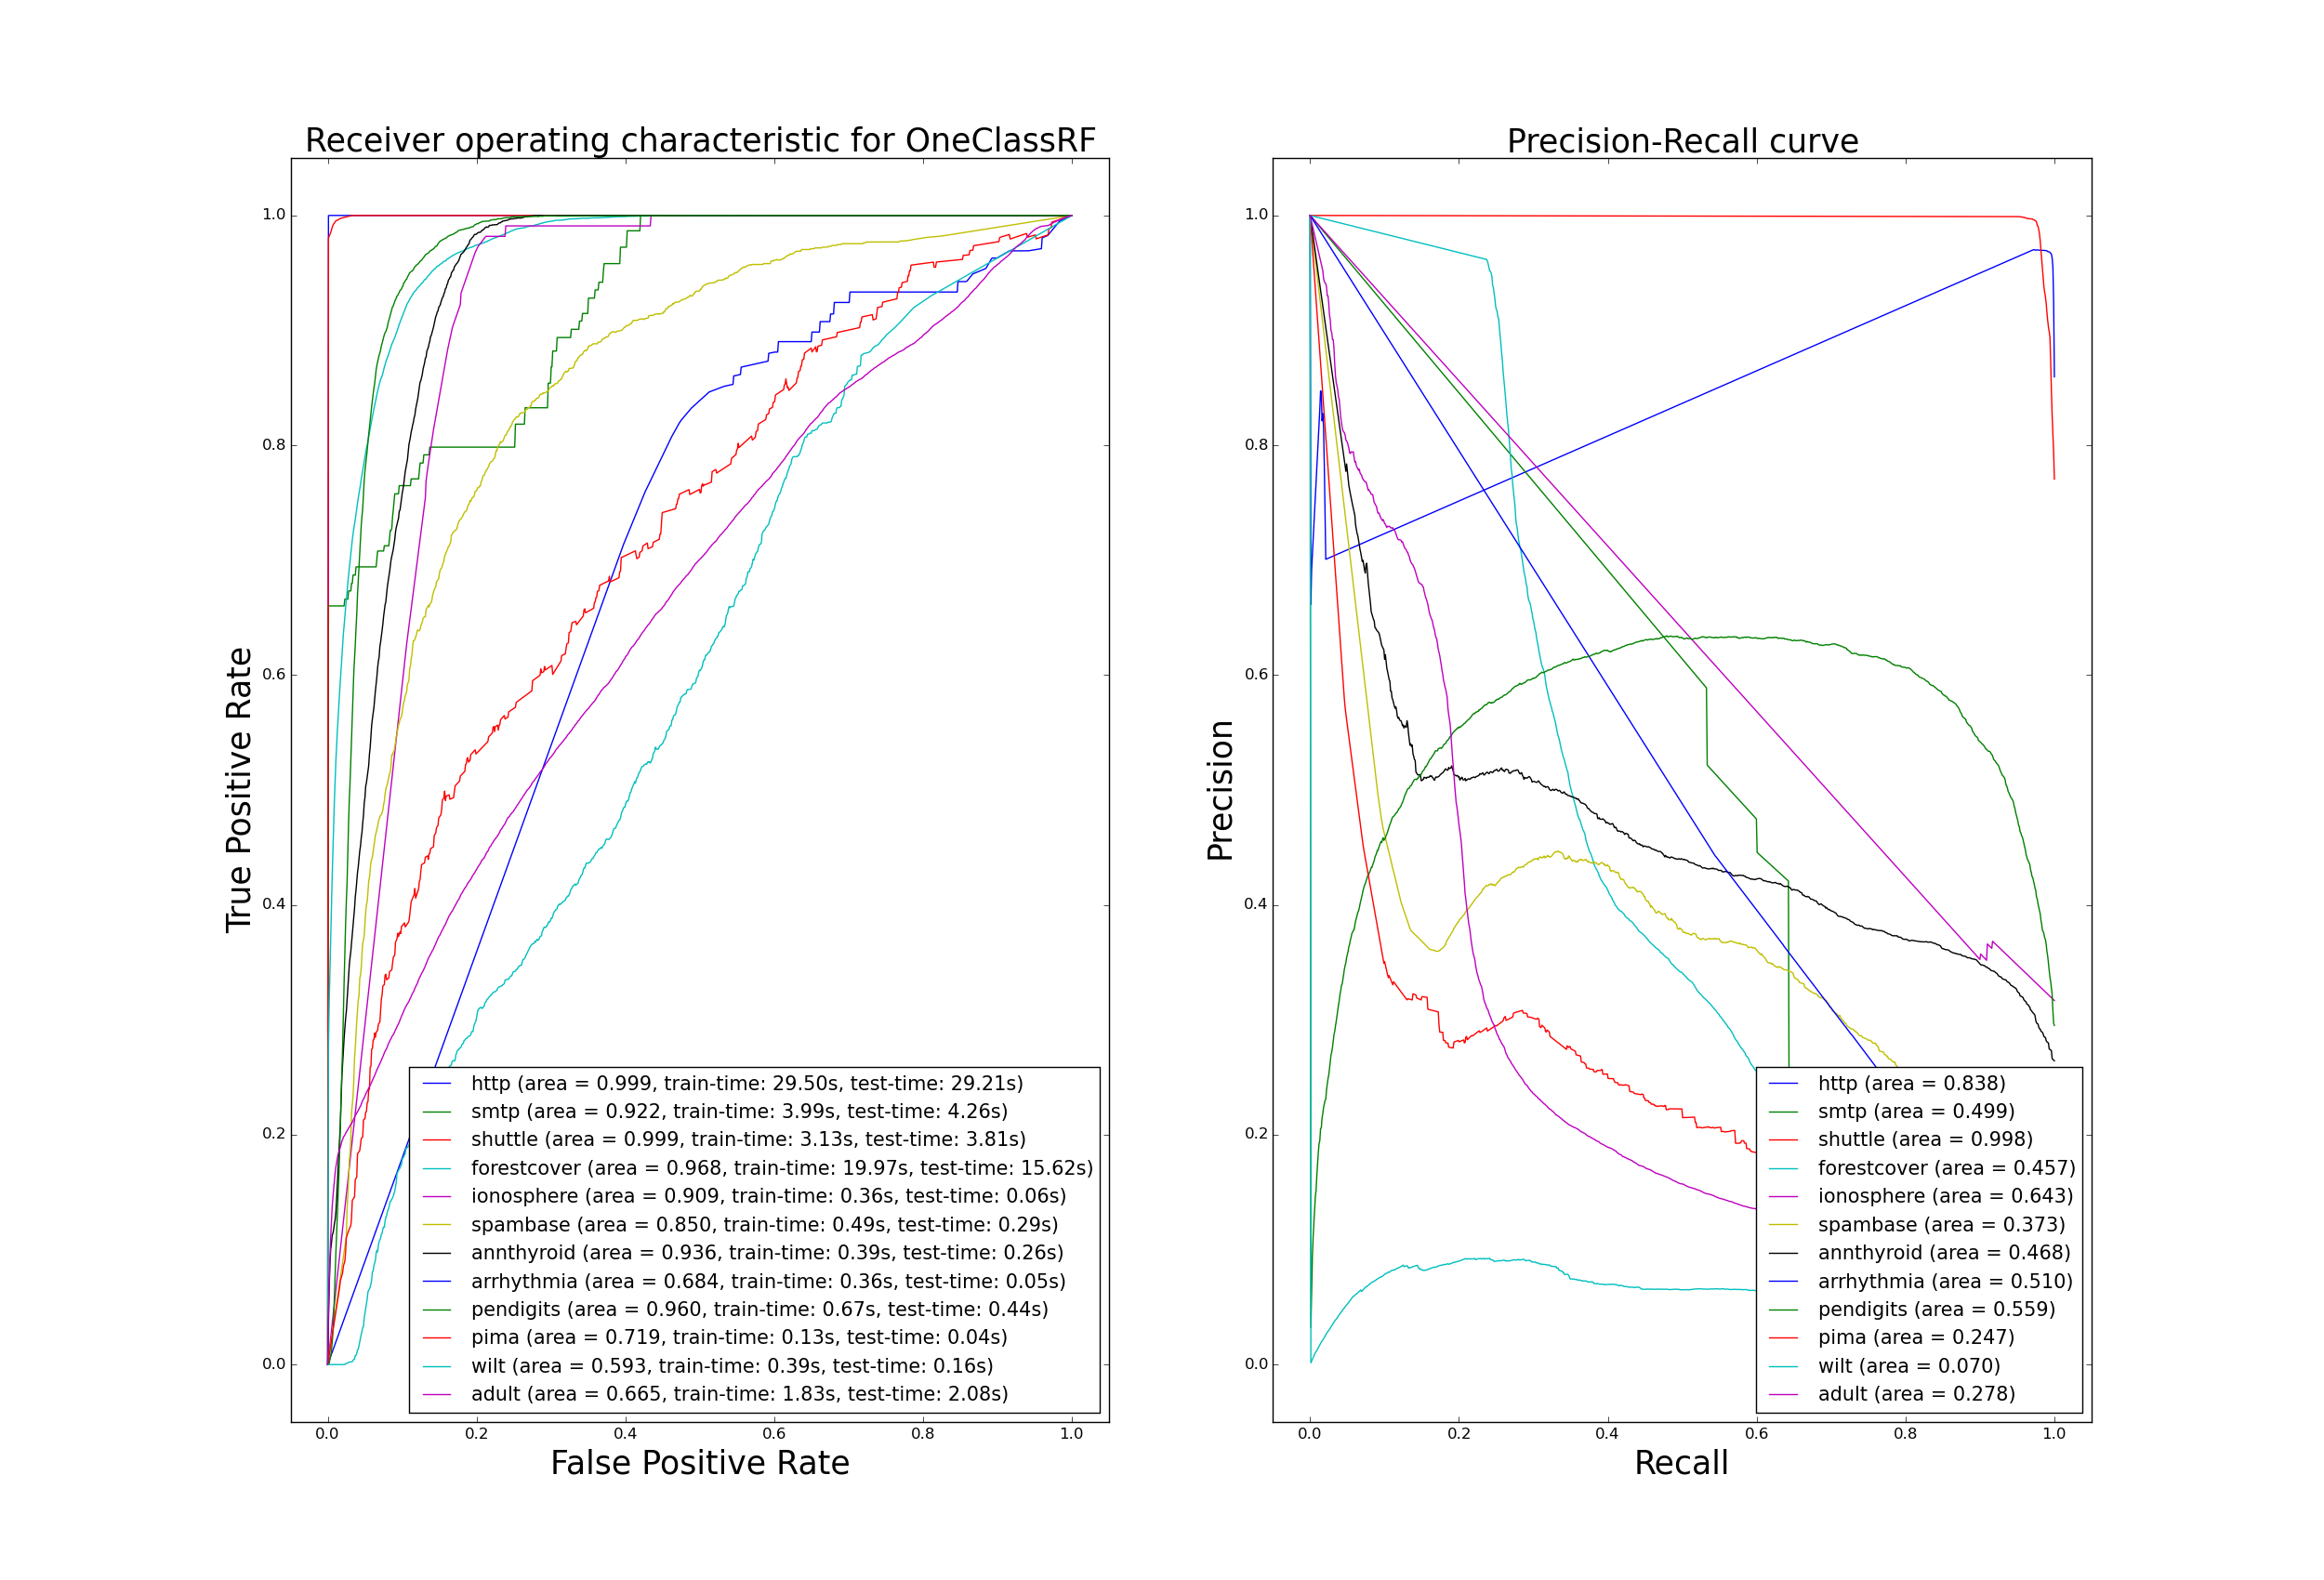
\includegraphics[trim=175 80 175 123, clip,
    width=0.75\textwidth]{./gfx/bench_oneclassrf_roc_pr_supervised_factorized.png}
\end{figure*}
\begin{figure*}[!ht]
    \caption{\acs{ROC} and \acs{PR} curves for \acs{OneClassRF} (outlier
    detection framework)}
    \label{ocrf:fig:oneclassrf_roc_pr_unsupervised}
    \centering
    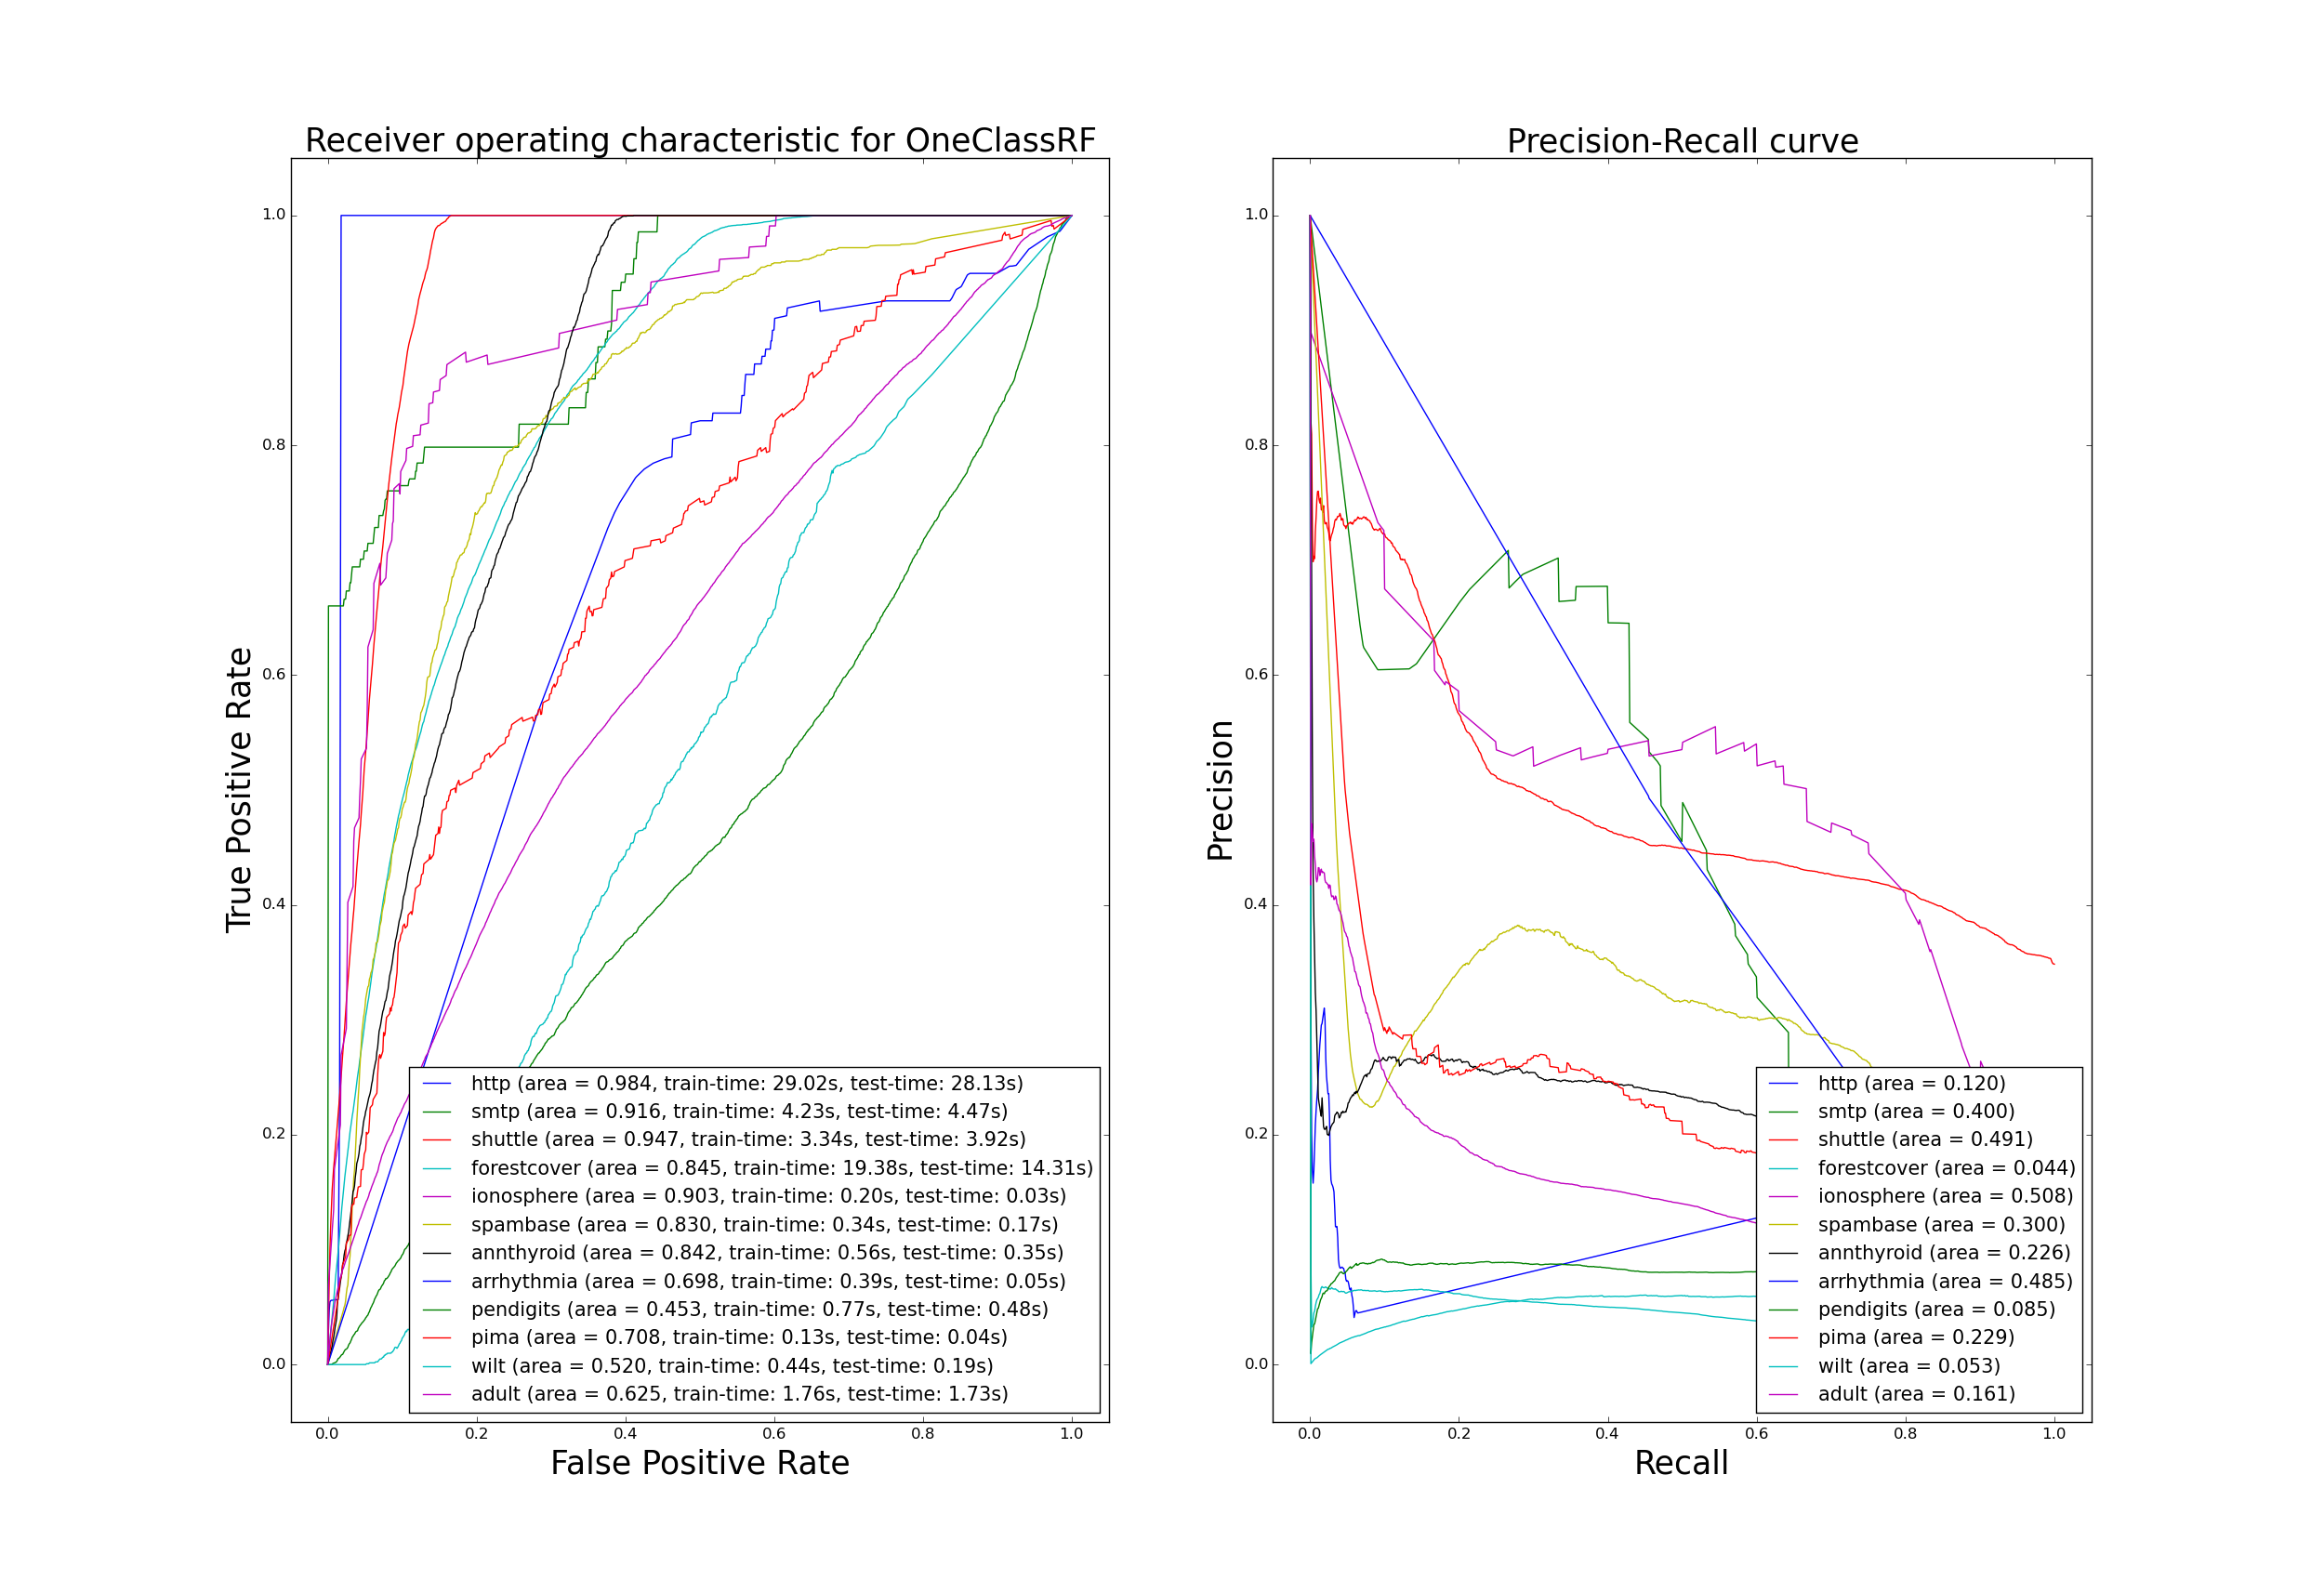
\includegraphics[trim=175 80 175 123, clip,
    width=0.75\textwidth]{./gfx/bench_oneclassrf_roc_pr_unsupervised_factorized.png}
\end{figure*}
\begin{figure*}[!ht]
    \caption{\acs{ROC} and \acs{PR} curves for \acs{iForest} (novelty detection
    framework)}
    \label{ocrf:fig:iforest_roc_pr}
    \centering
    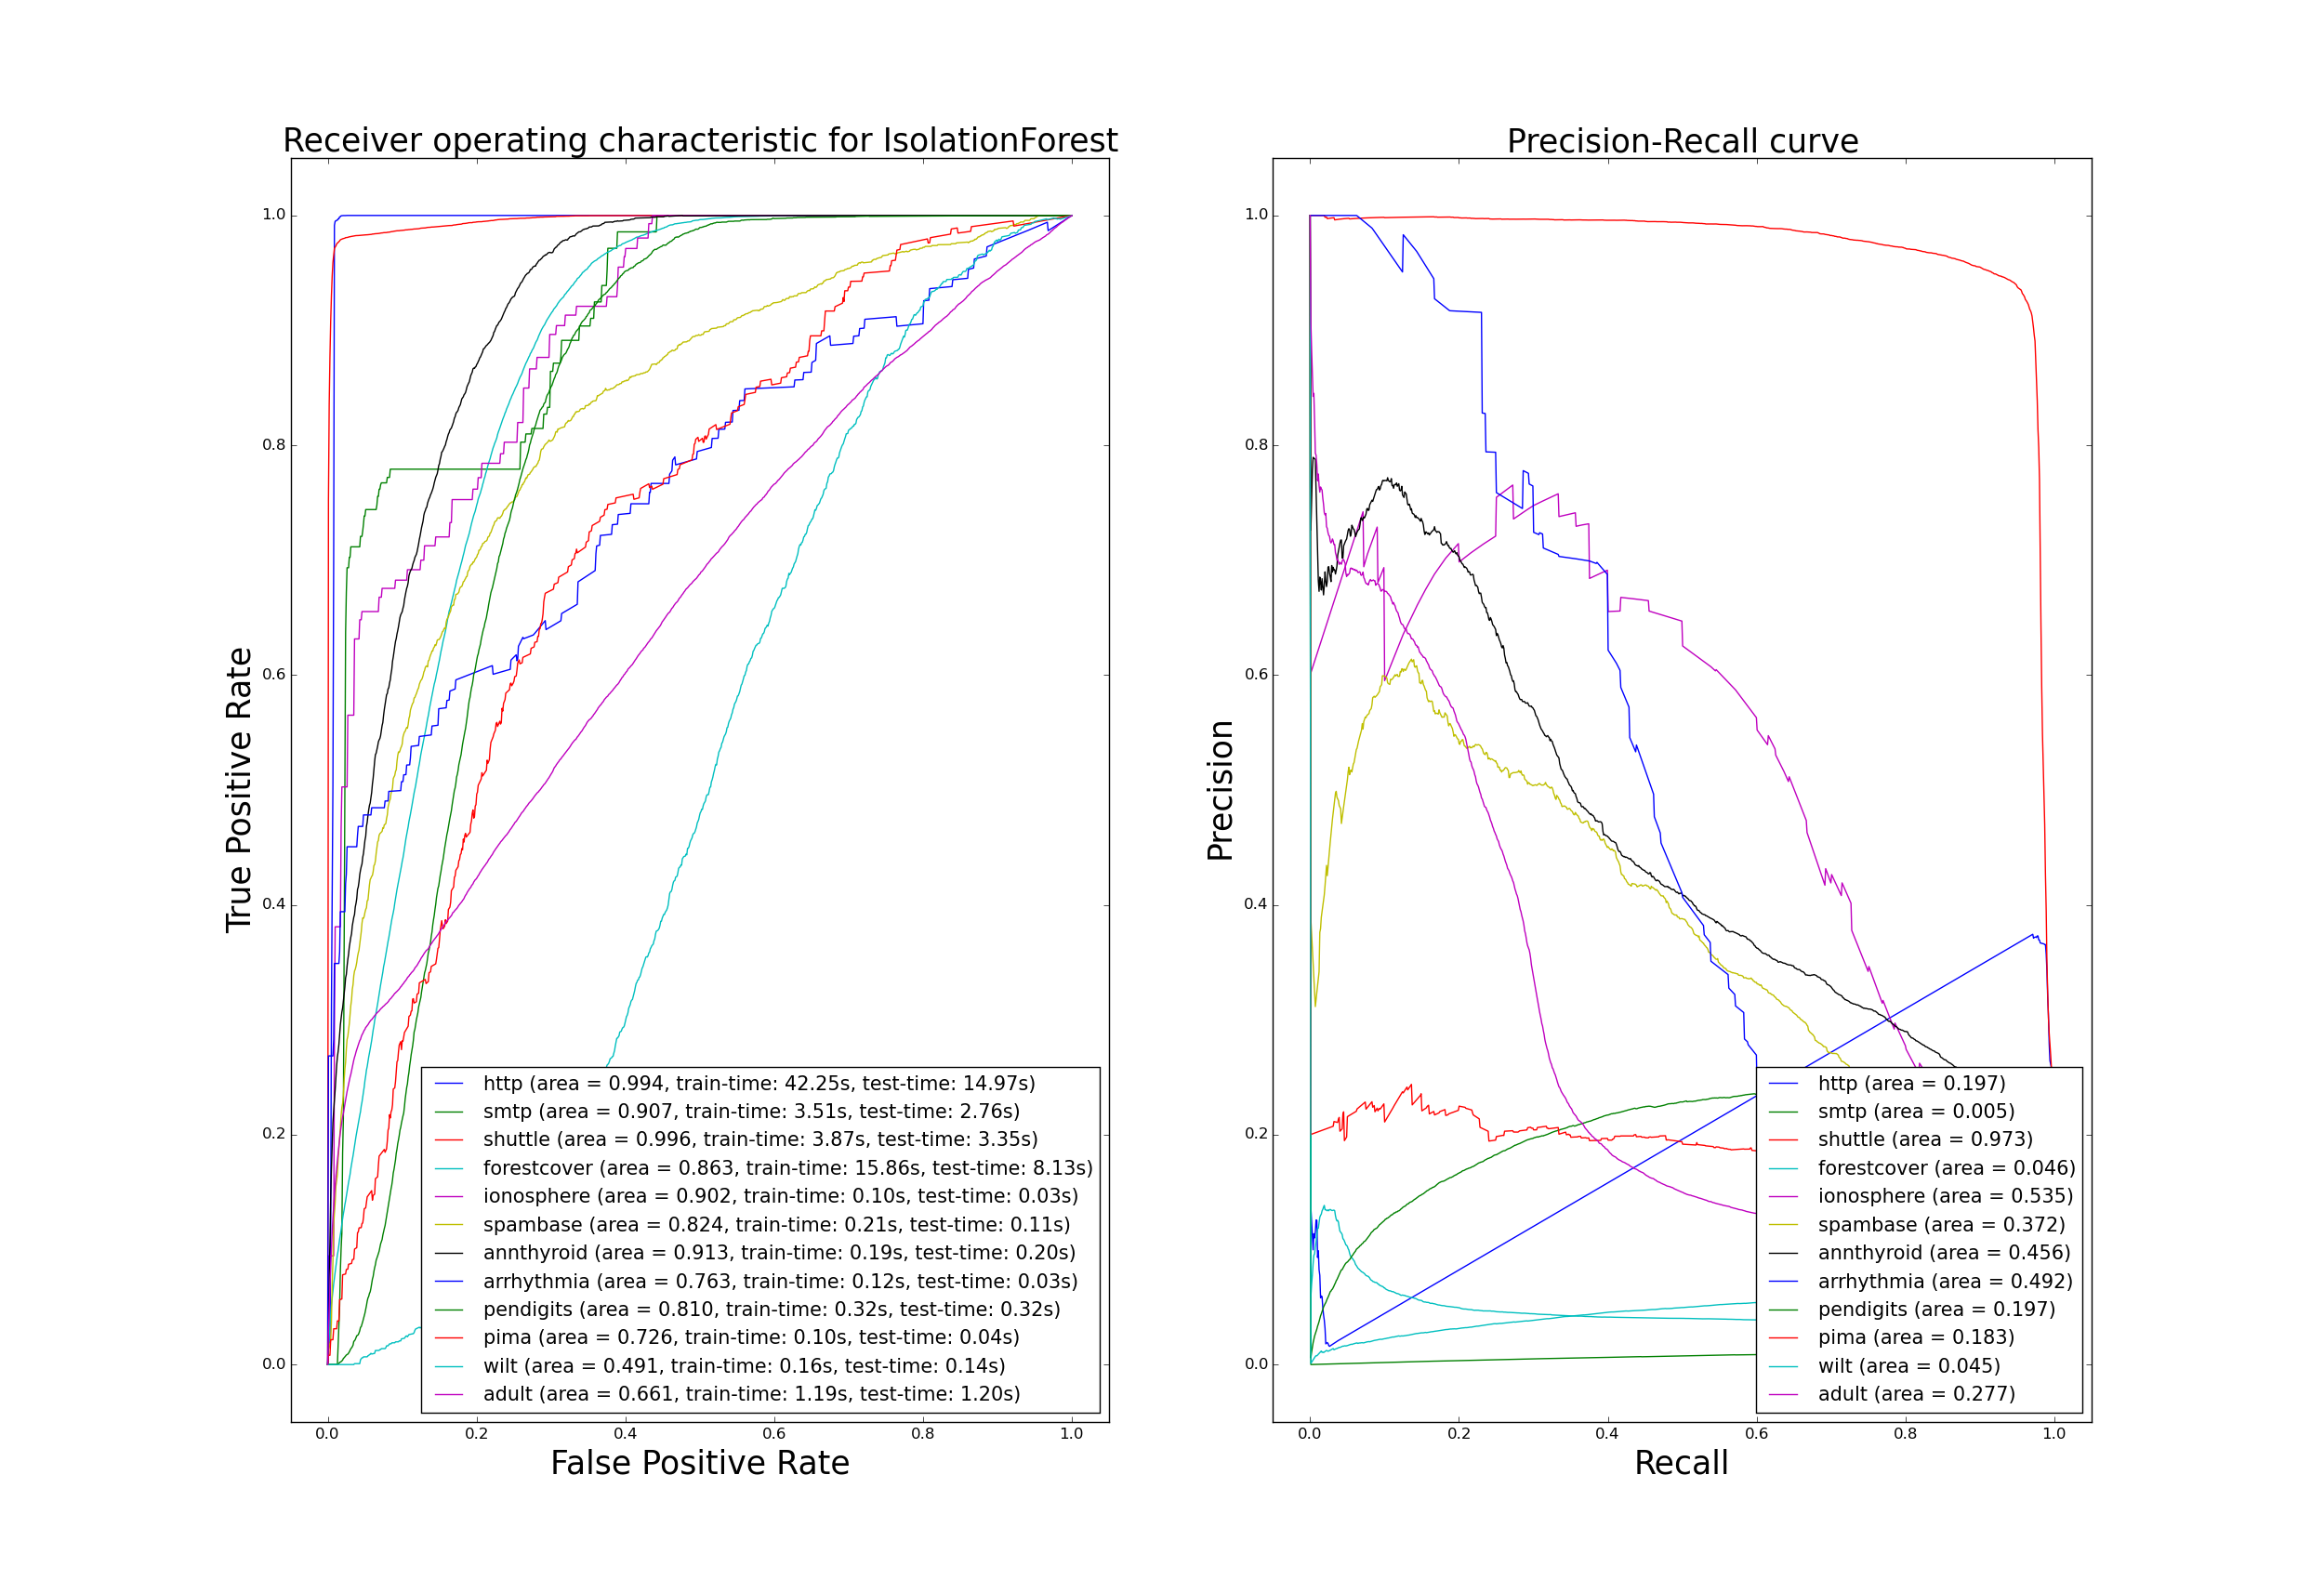
\includegraphics[trim=175 80 175 123, clip,
    width=0.75\textwidth]{./gfx/bench_iforest_roc_pr_supervised_factorized.png}
\end{figure*}
\begin{figure*}[!ht]
    \caption{\acs{ROC} and \acs{PR} curves for \acs{iForest} (outlier detection
    framework)}
    \label{ocrf:fig:iforest_roc_pr_unsupervised}
    \centering
    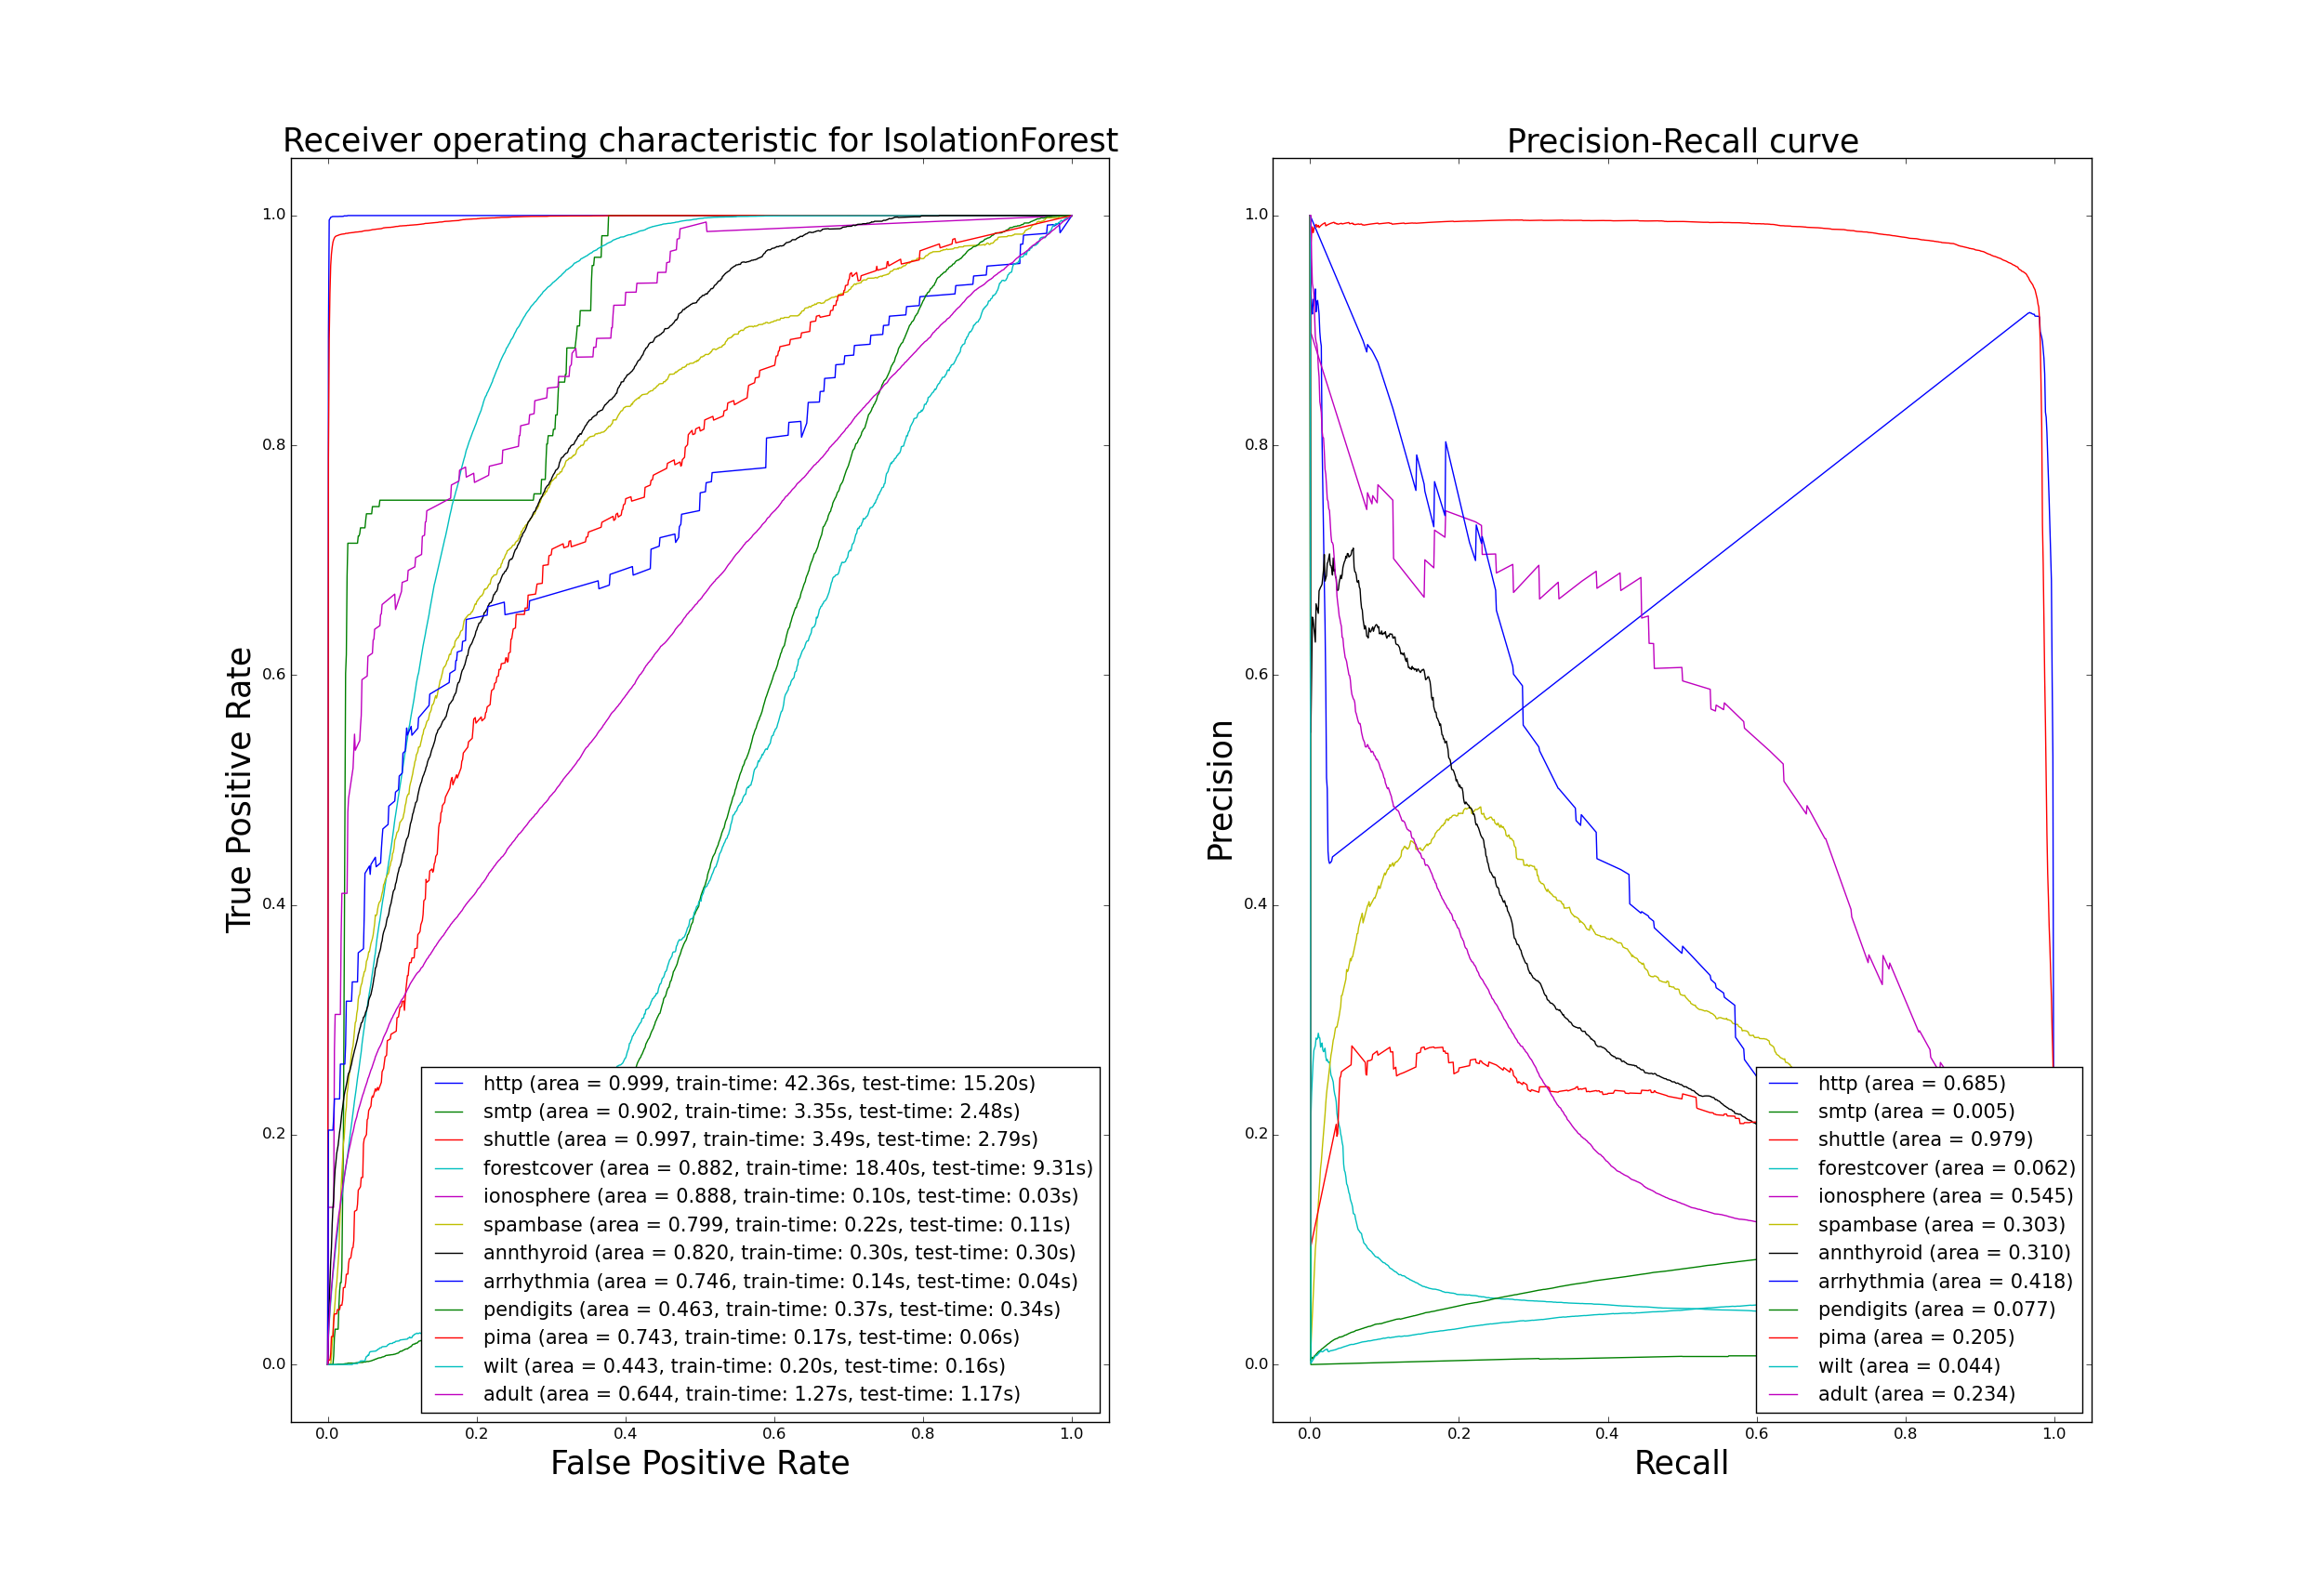
\includegraphics[trim=175 80 175 123, clip,
    width=0.75\textwidth]{./gfx/bench_iforest_roc_pr_unsupervised_factorized.png}
\end{figure*}
\begin{figure*}[!ht]
    \caption{\acs{ROC} and \acs{PR} curves for \acs{OCRFsampling} (novelty
    detection framework)}
    \label{ocrf:fig:ocrfm_roc_pr}
    \centering
    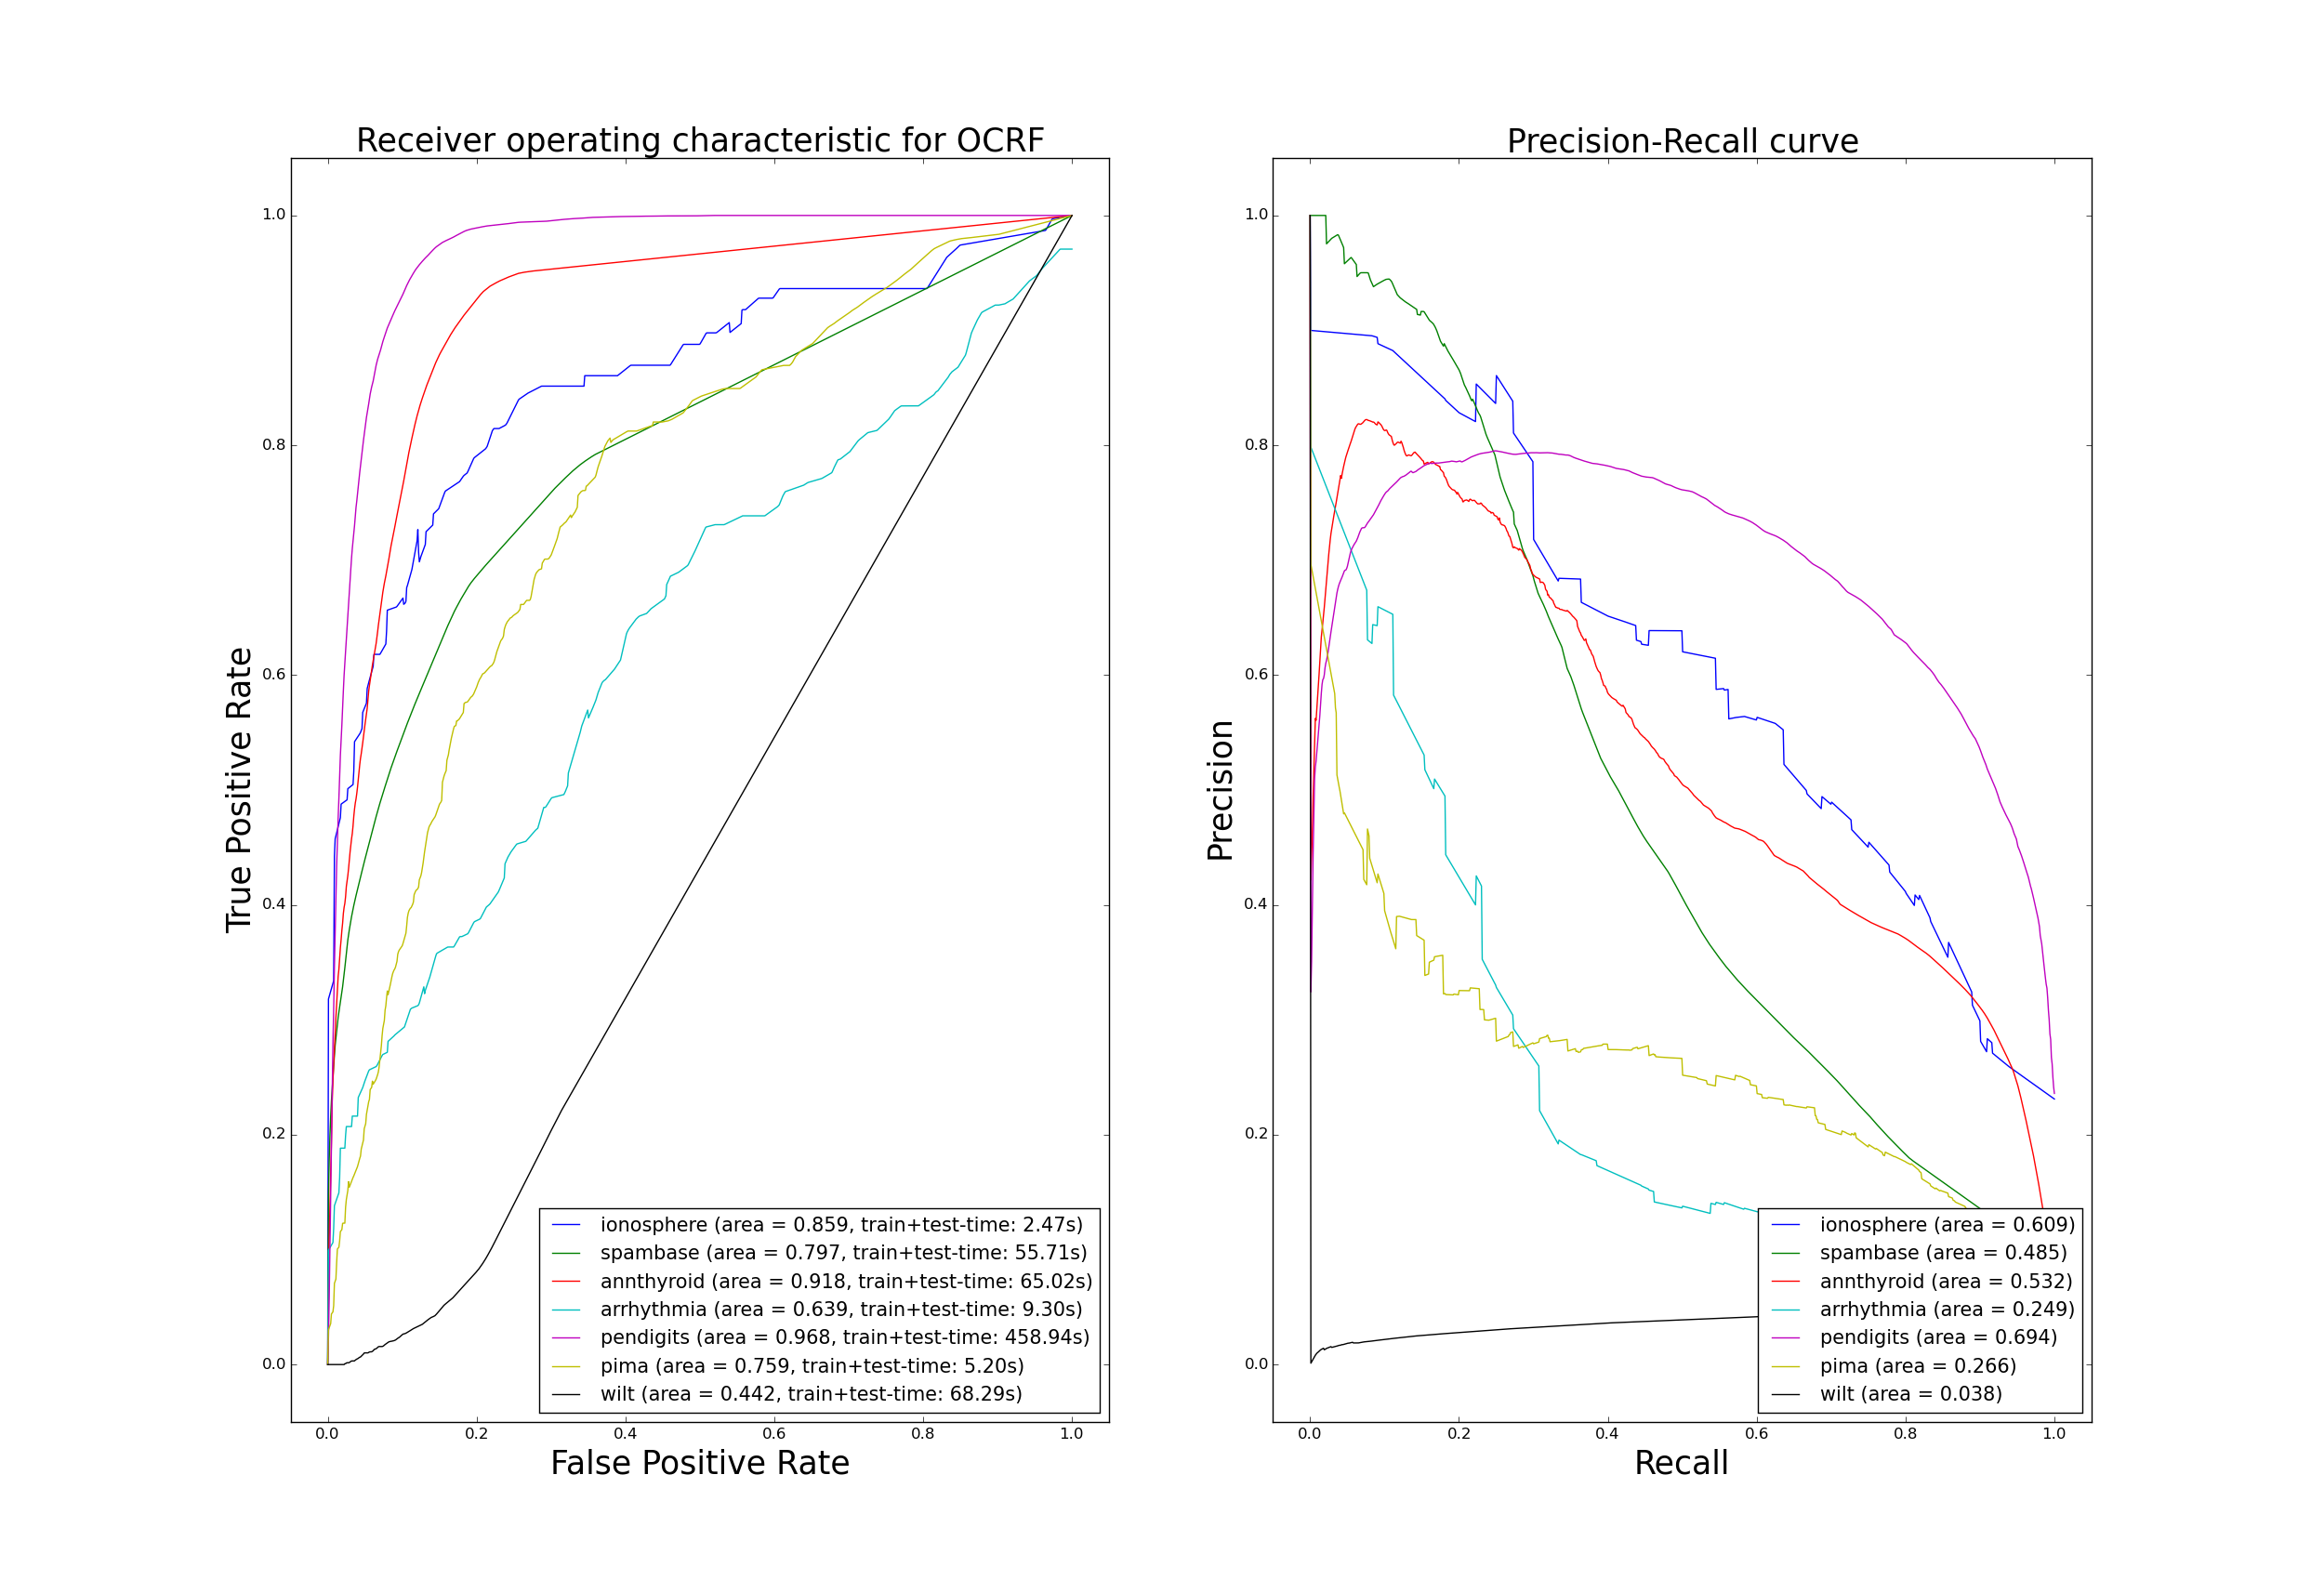
\includegraphics[trim=175 80 175 123, clip,
    width=0.75\textwidth]{./gfx/bench_ocrf_roc_pr_supervised_factorized.png}
\end{figure*}
\begin{figure*}[!ht]
    \caption{\acs{ROC} and \acs{PR} curves for \acs{OCRFsampling} (outlier
    detection framework)}
    \label{ocrf:fig:ocrfm_roc_pr_unsupervised}
    \centering
    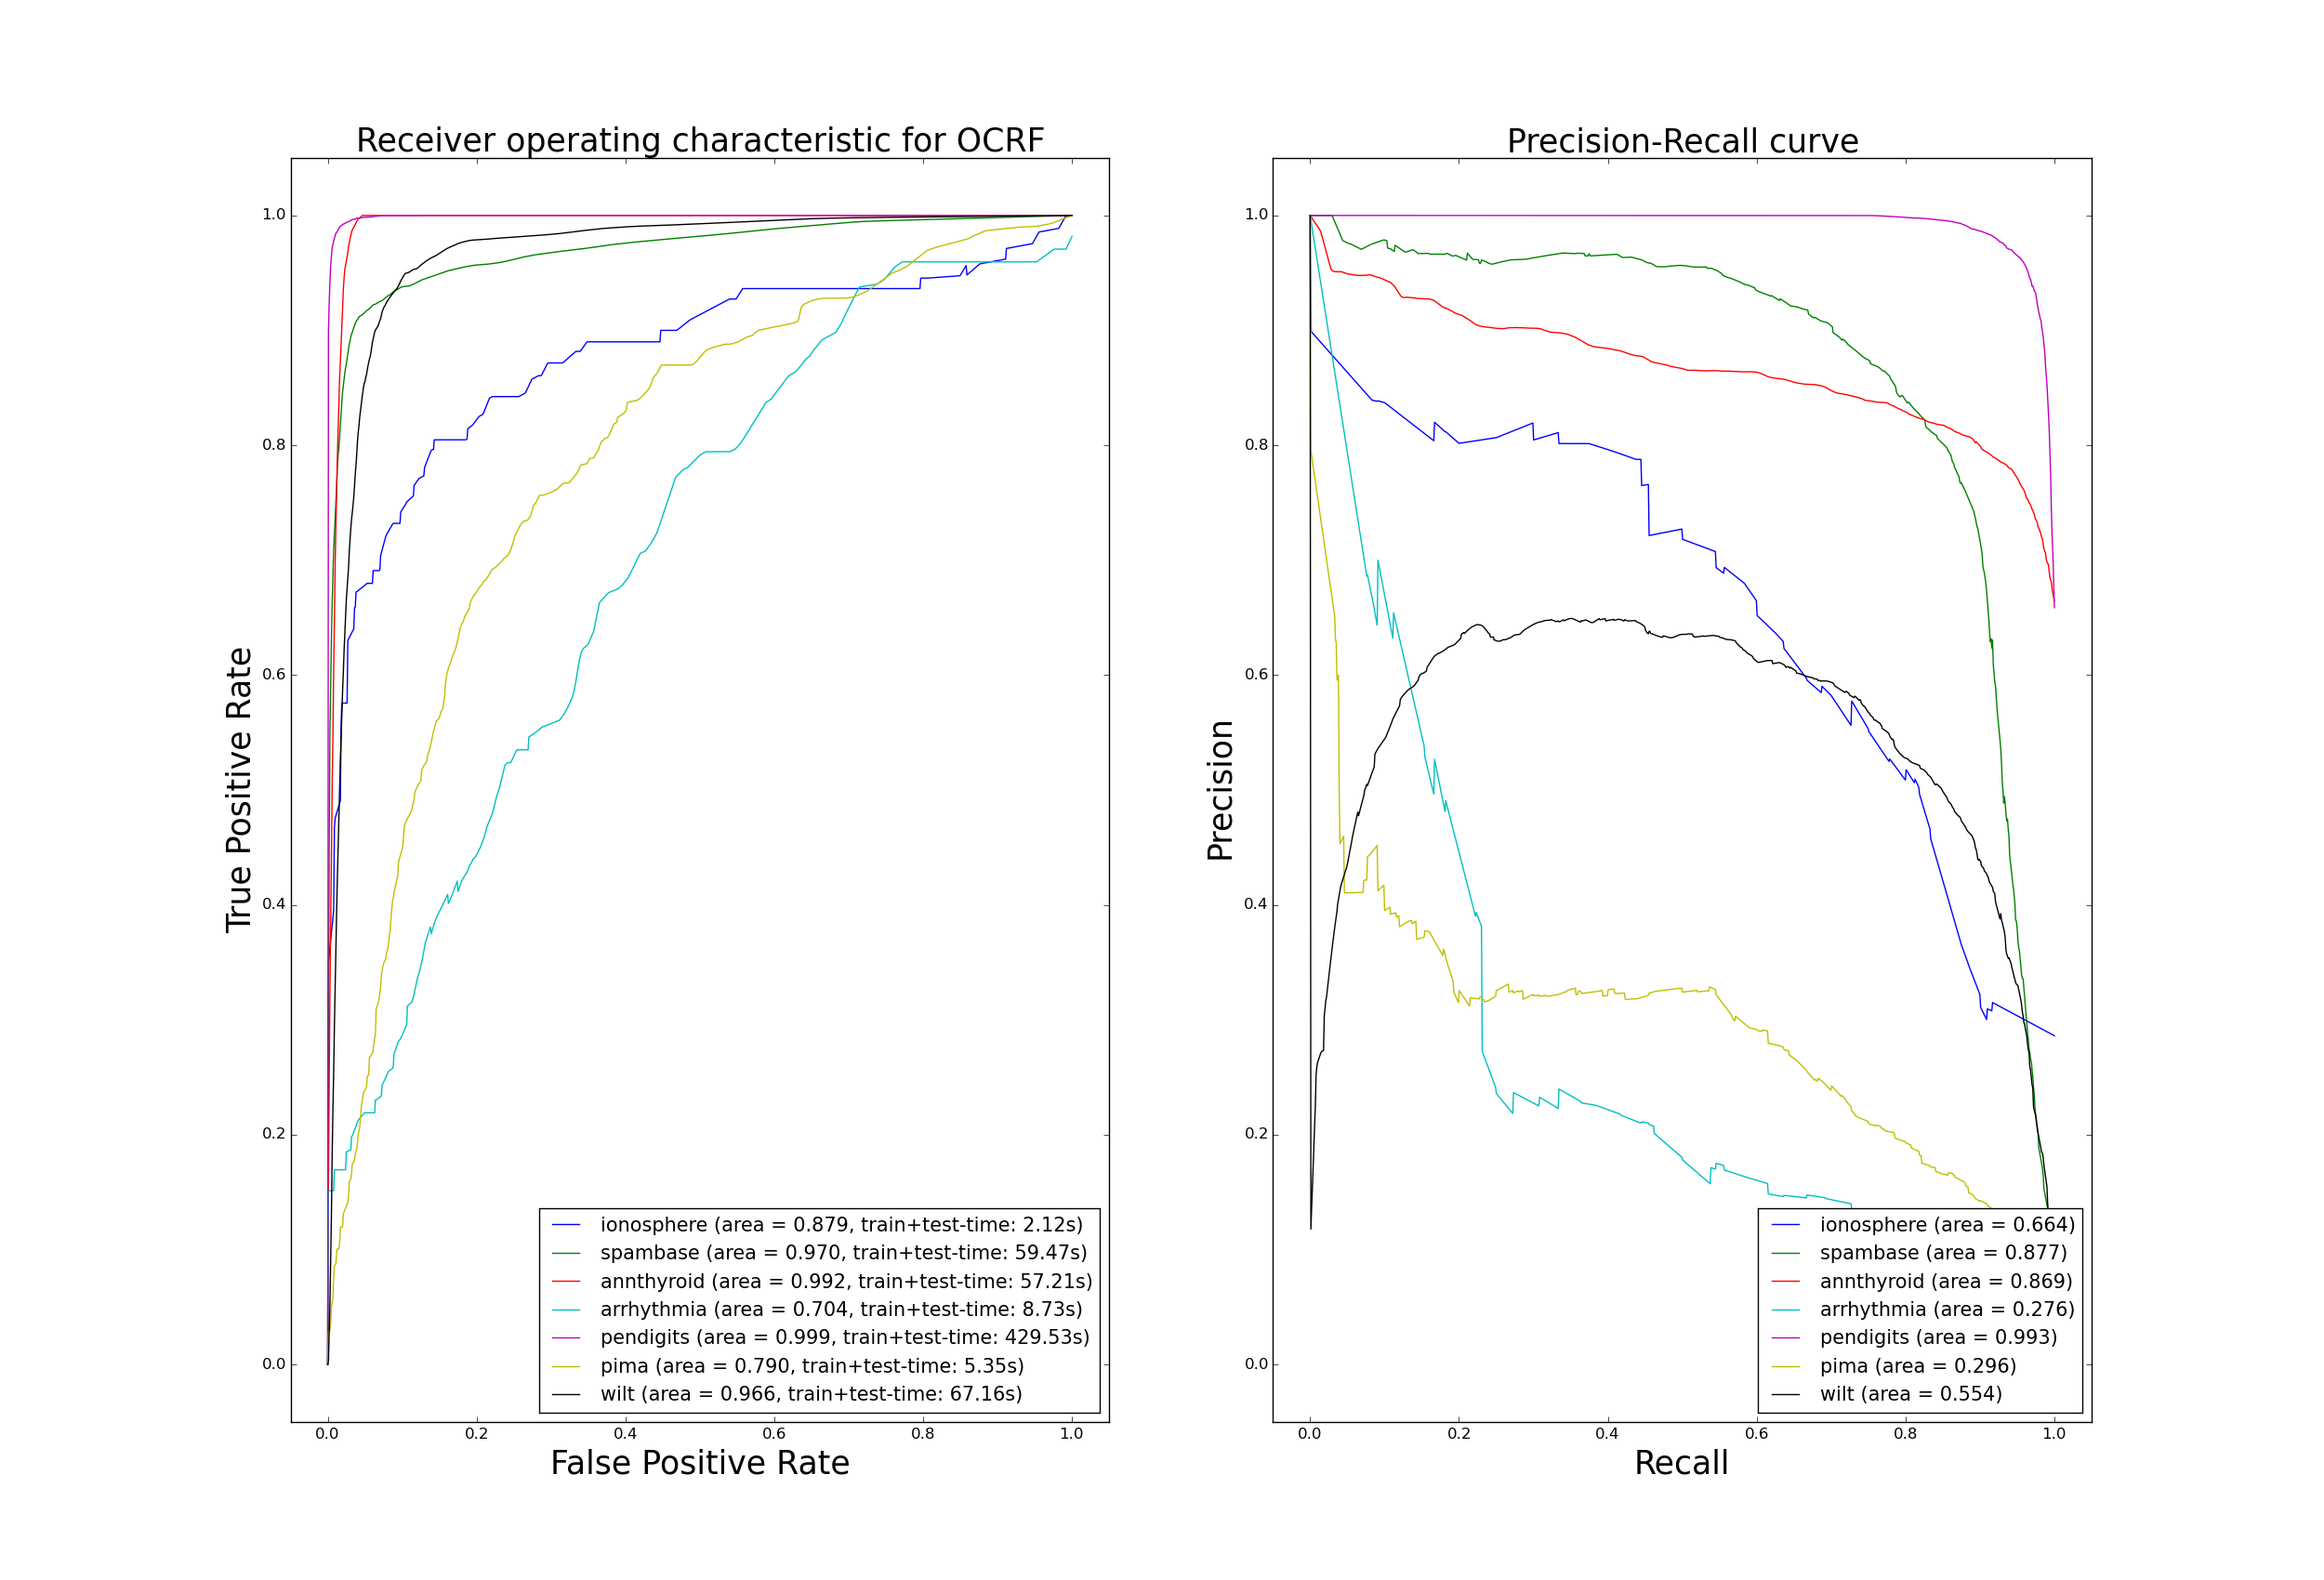
\includegraphics[trim=175 80 175 123, clip,
    width=0.75\textwidth]{./gfx/bench_ocrf_roc_pr_unsupervised_factorized.png}
\end{figure*}
\begin{figure*}[!ht]
    \caption{\acs{ROC} and \acs{PR} curves for \acs{OCSVM} (novelty detection
    framework)}
    \label{ocrf:fig:ocsvm_roc_pr}
    \centering
    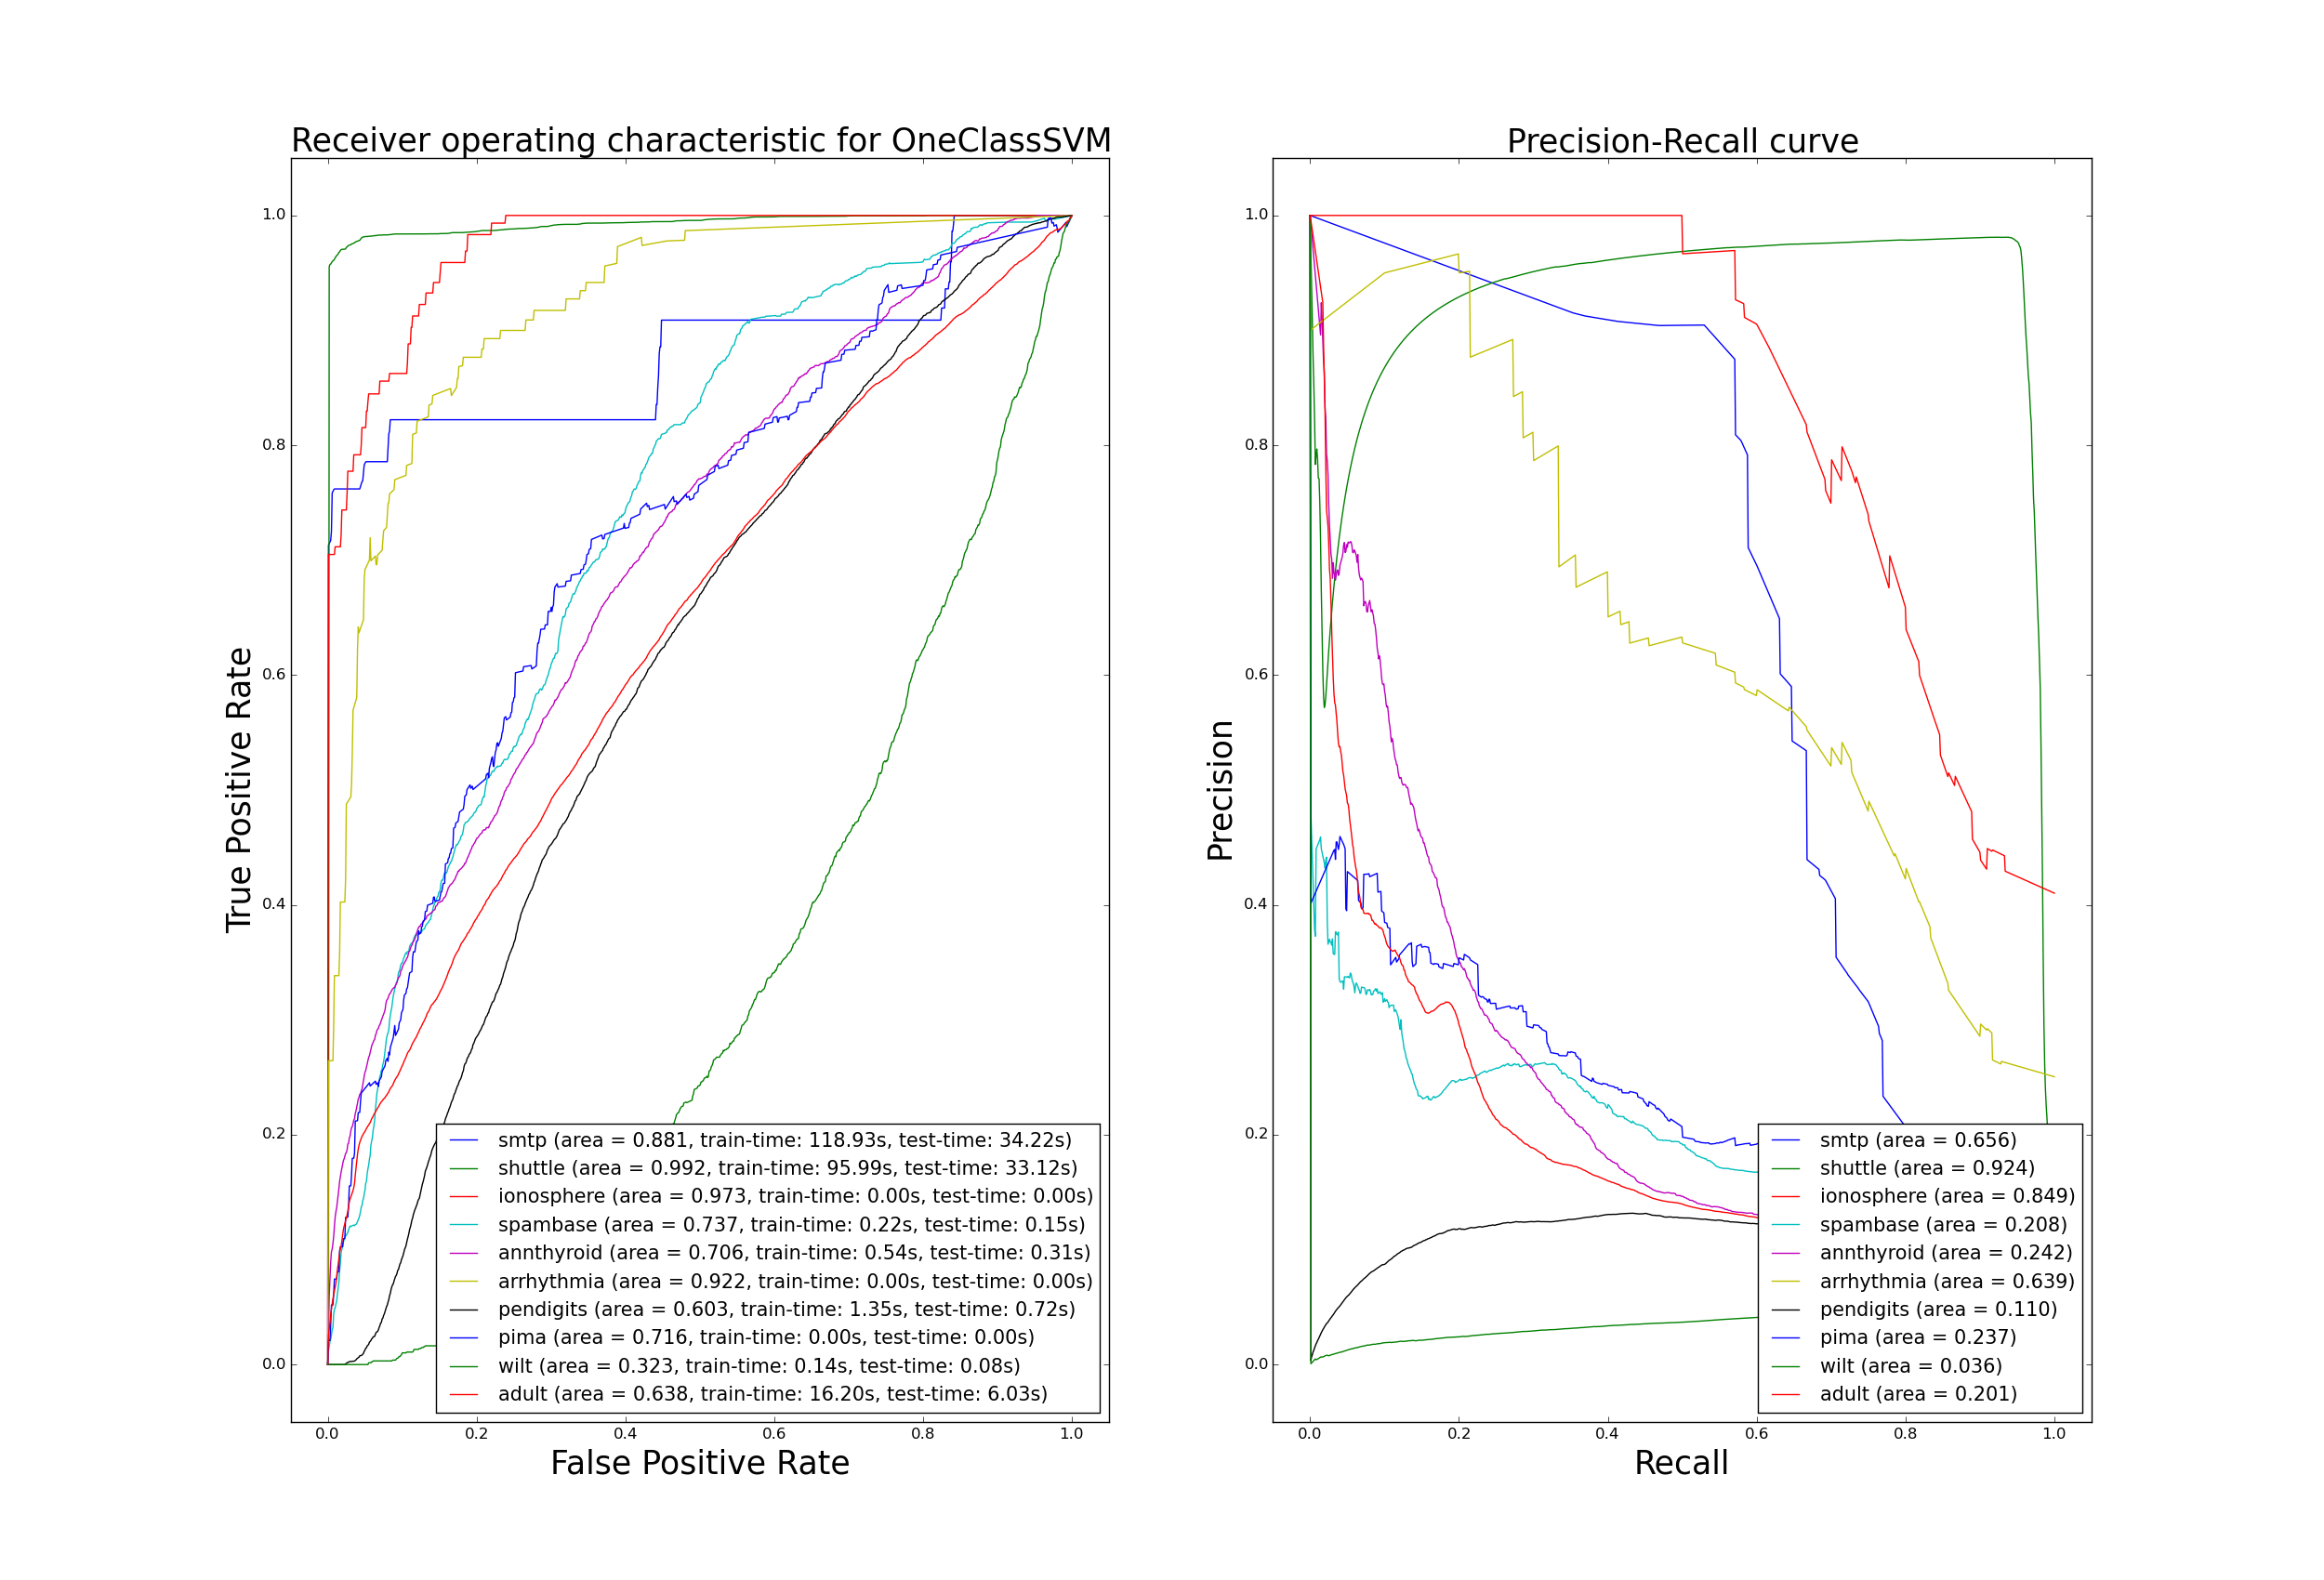
\includegraphics[trim=175 80 175 123, clip,
    width=0.75\textwidth]{./gfx/bench_ocsvm_roc_pr_supervised_factorized.png}
\end{figure*}
\begin{figure*}[!ht]
    \caption{\acs{ROC} and \acs{PR} curves for \acs{OCSVM} (outlier detection
    framework)}
    \label{ocrf:fig:ocsvm_roc_pr_unsupervised}
    \centering
    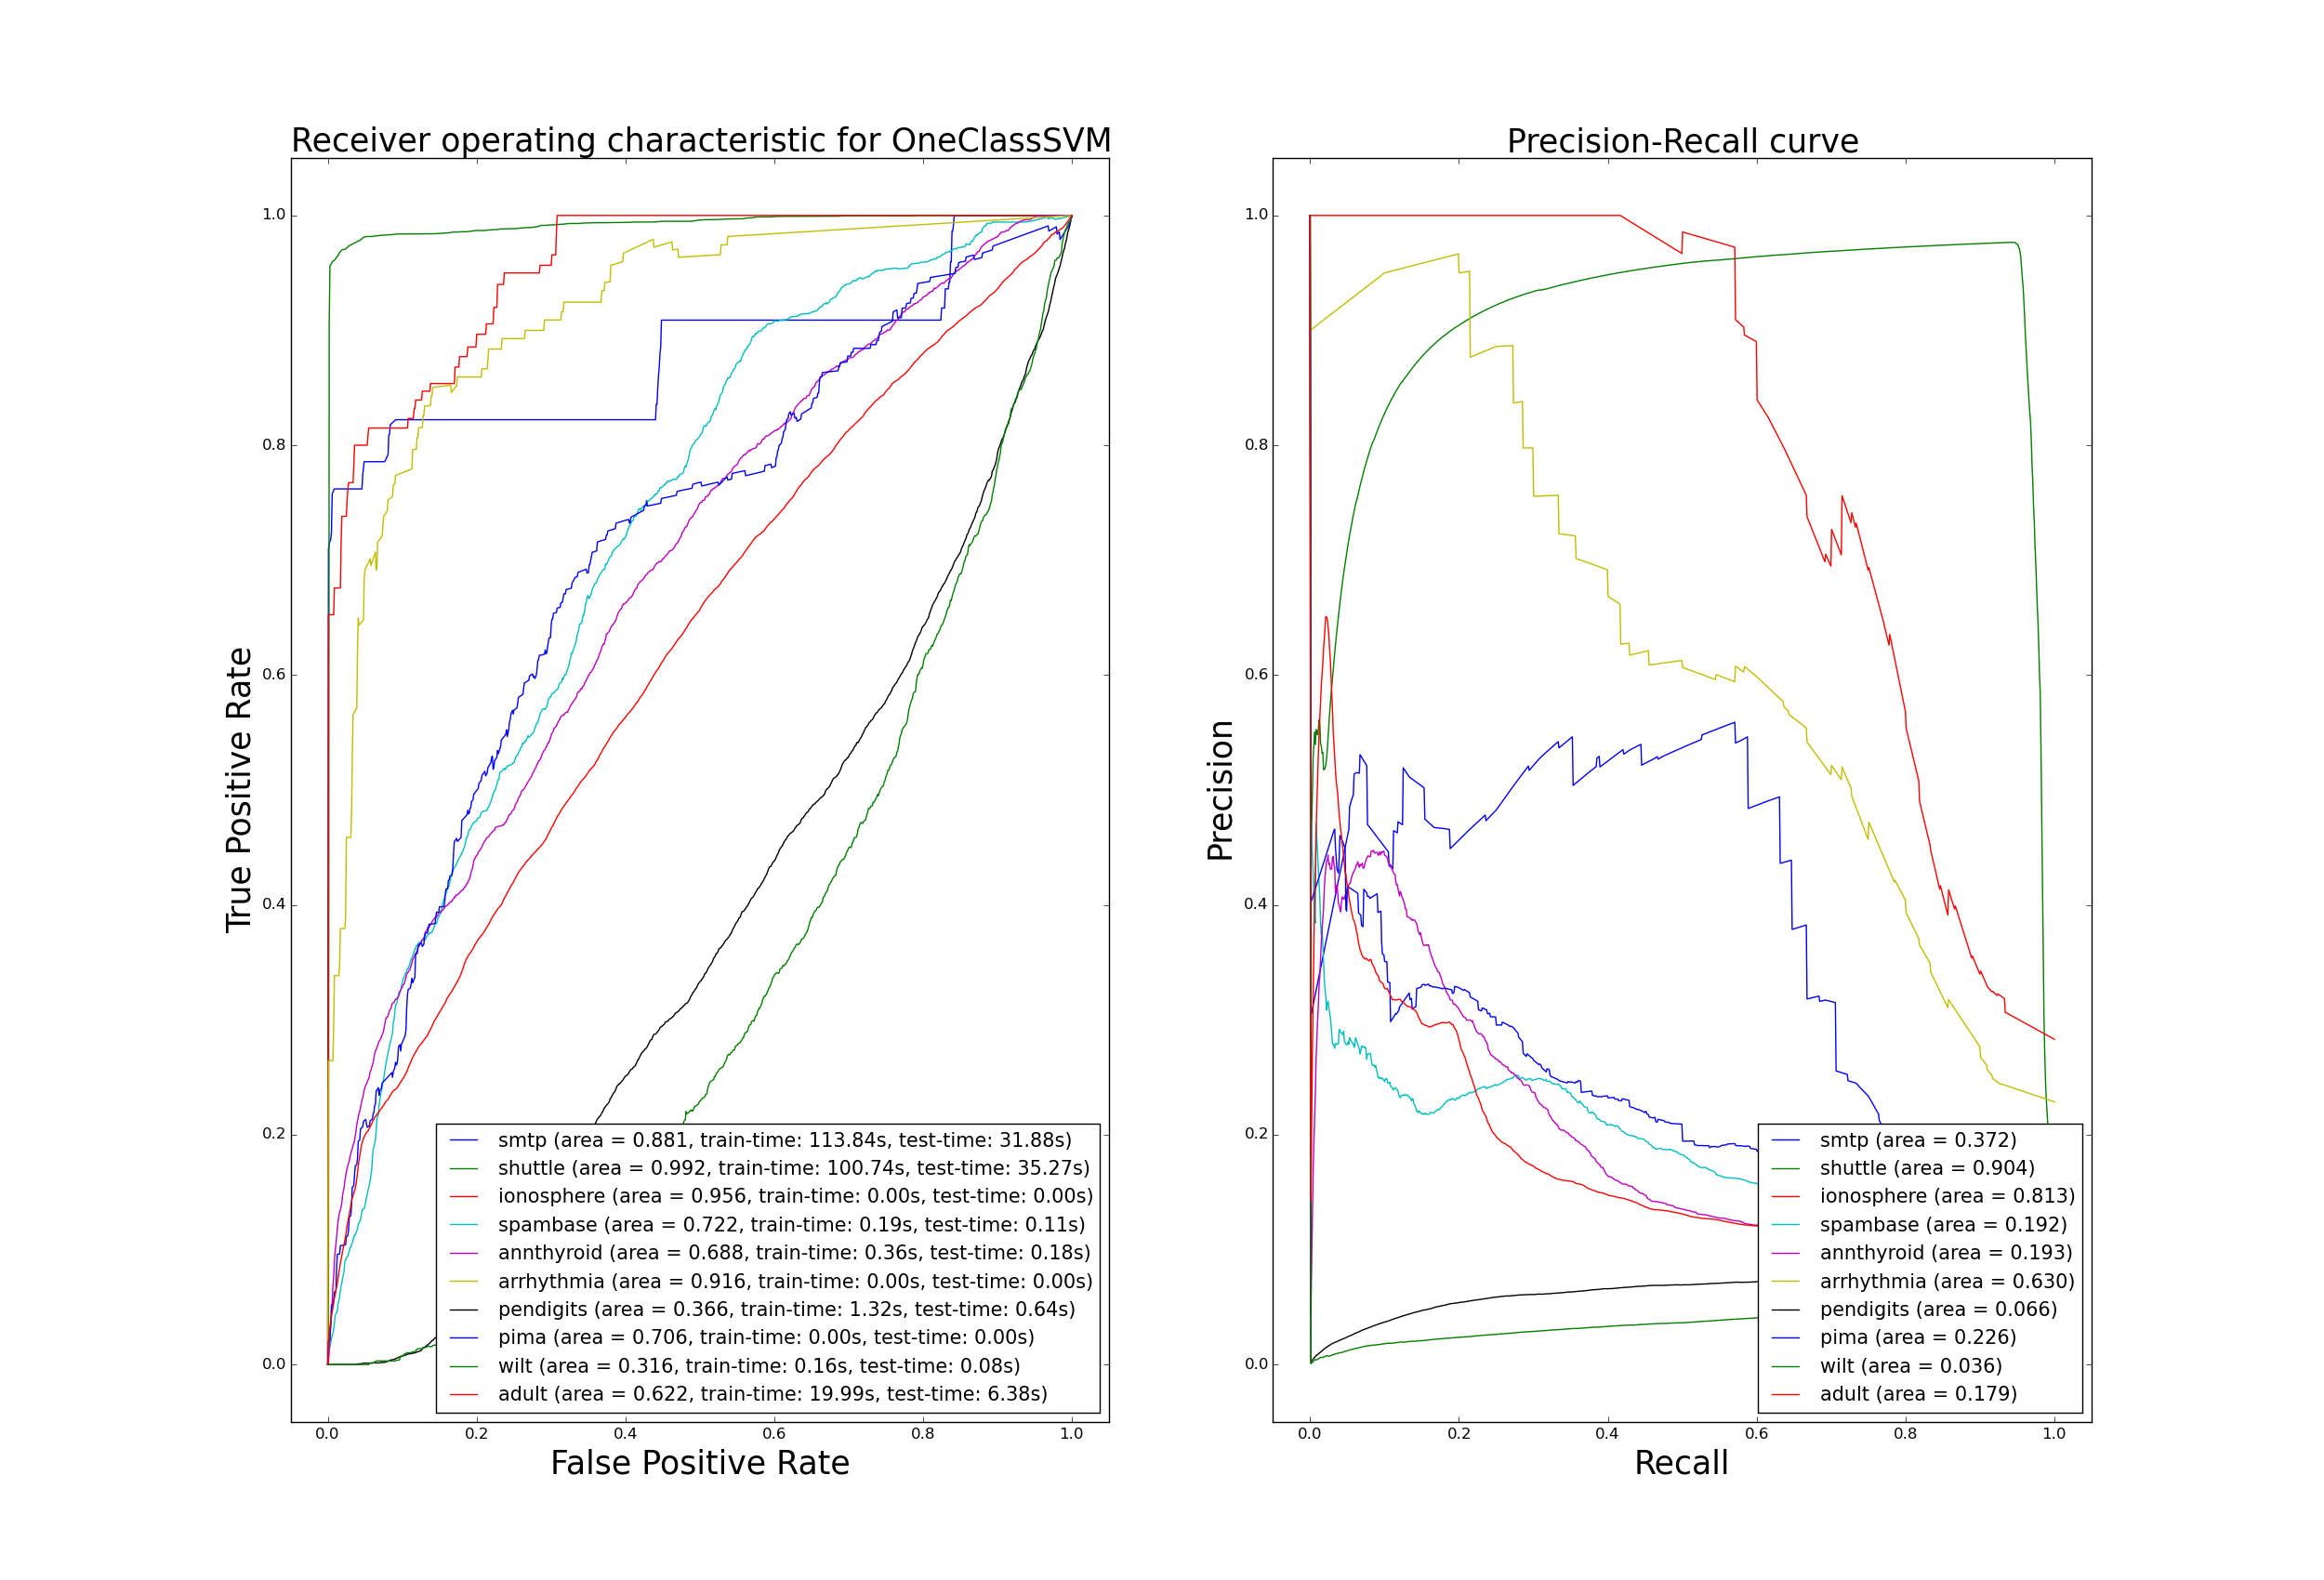
\includegraphics[trim=175 80 175 123, clip,
    width=0.75\textwidth]{./gfx/bench_ocsvm_roc_pr_unsupervised_factorized.png}
\end{figure*}
\begin{figure*}[!ht]
    \caption{\acs{ROC} and \acs{PR} curves for \acs{LOF} (novelty detection
    framework)}
    \label{ocrf:fig:lof_roc_pr}
    \centering
    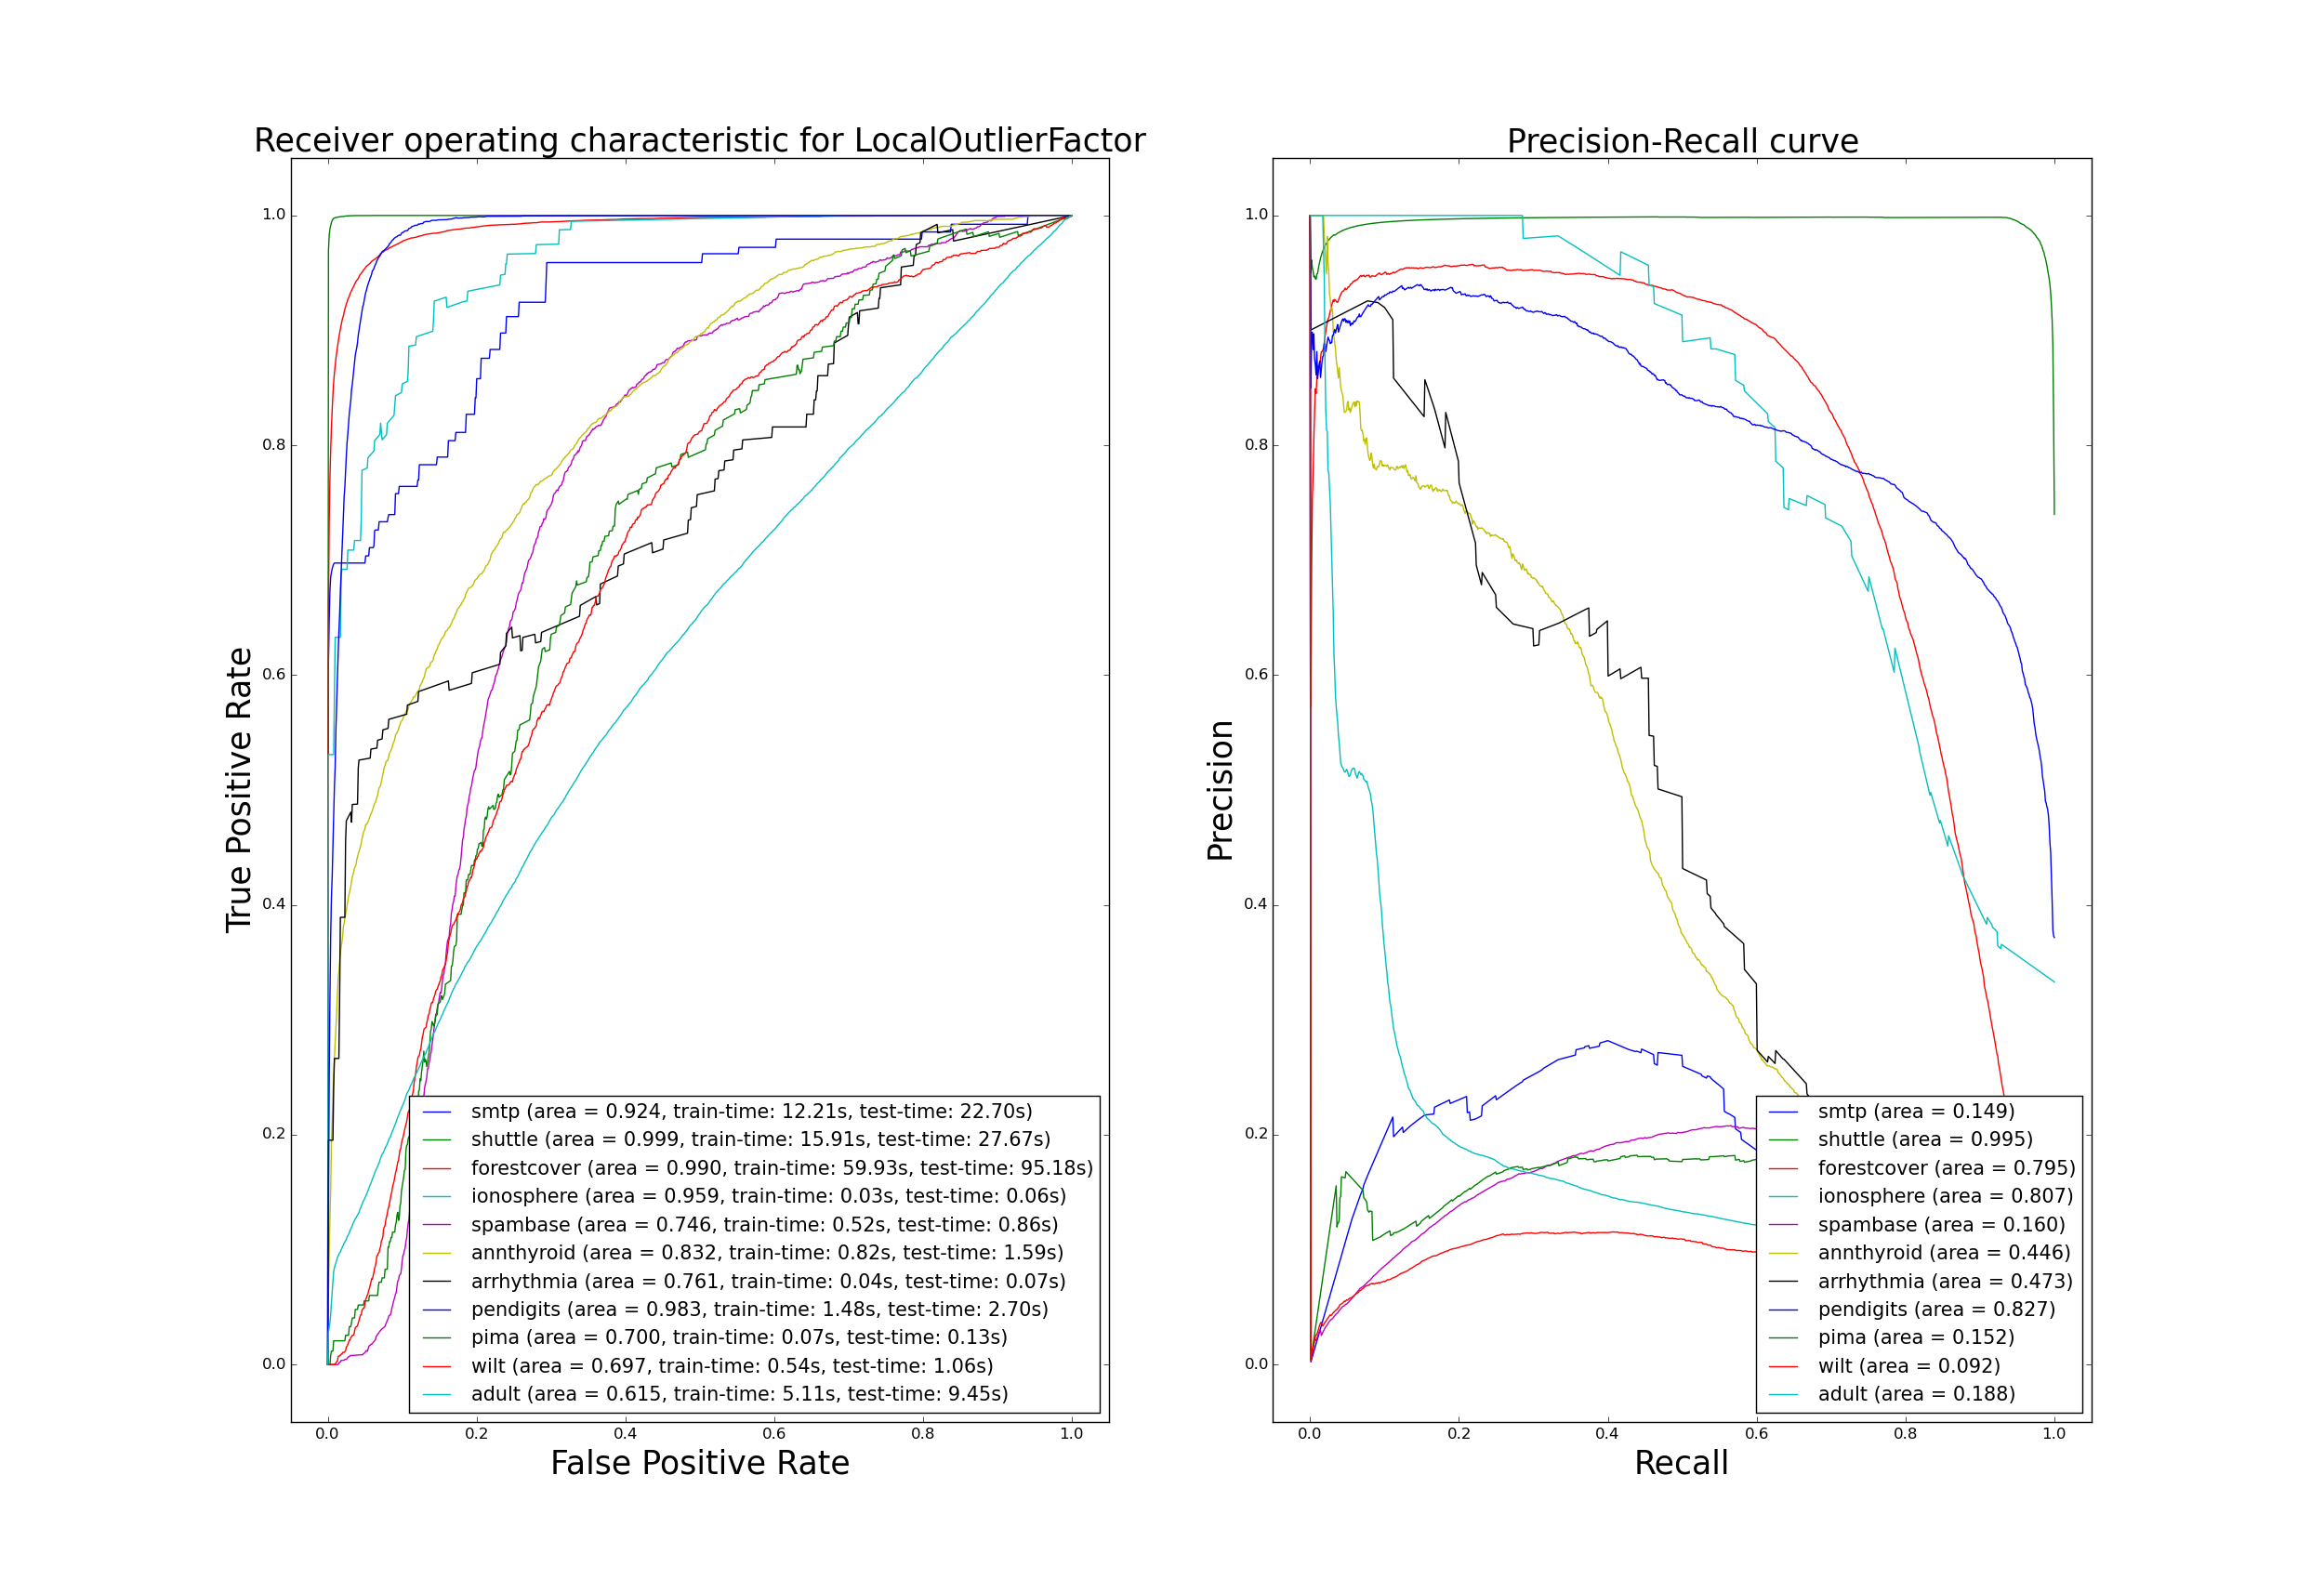
\includegraphics[trim=175 80 175 123, clip,
    width=0.75\textwidth]{./gfx/bench_lof_roc_pr_supervised_factorized.png}
\end{figure*}
\begin{figure*}[!ht]
    \caption{\acs{ROC} and \acs{PR} curves for \acs{LOF} (outlier detection
    framework)}
    \label{ocrf:fig:lof_roc_pr_unsupervised}
    \centering
    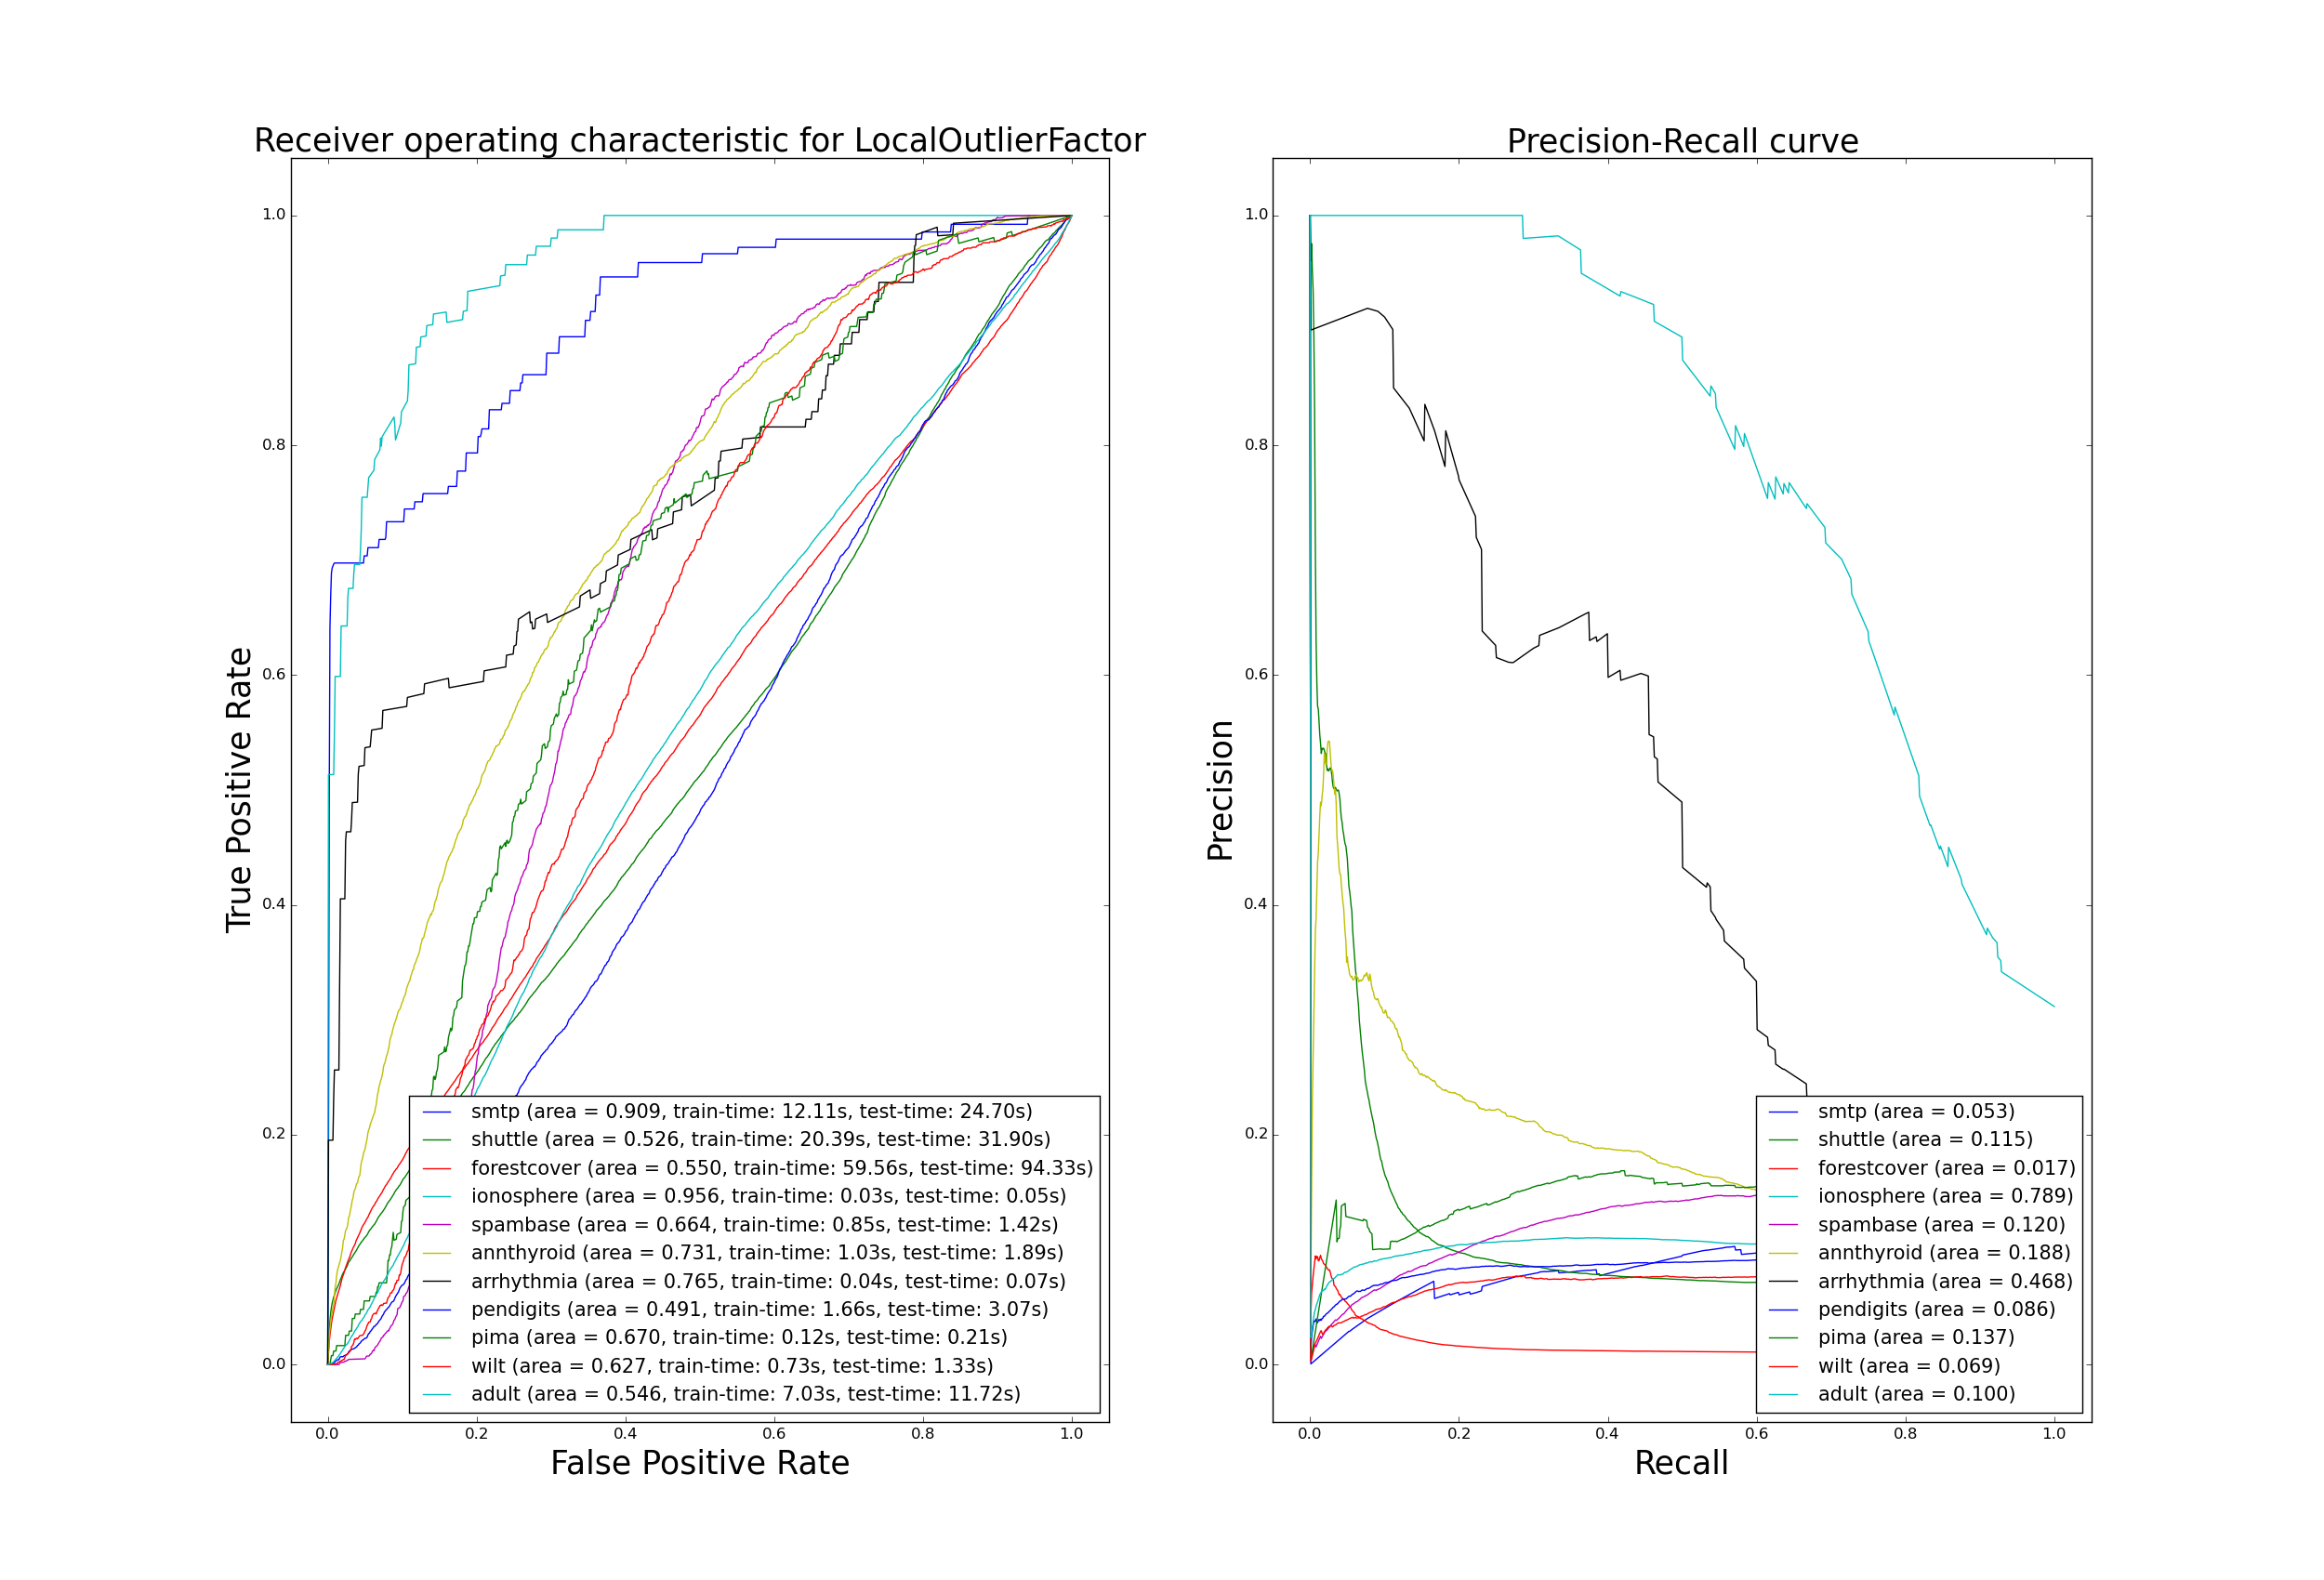
\includegraphics[trim=175 80 175 123, clip,
    width=0.75\textwidth]{./gfx/bench_lof_roc_pr_unsupervised_factorized.png}
\end{figure*}
\begin{figure*}[!ht]
    \caption{\acs{ROC} and \acs{PR} curves for Orca (novelty detection
    framework)}
    \label{ocrf:fig:orca_roc_pr}
    \centering
    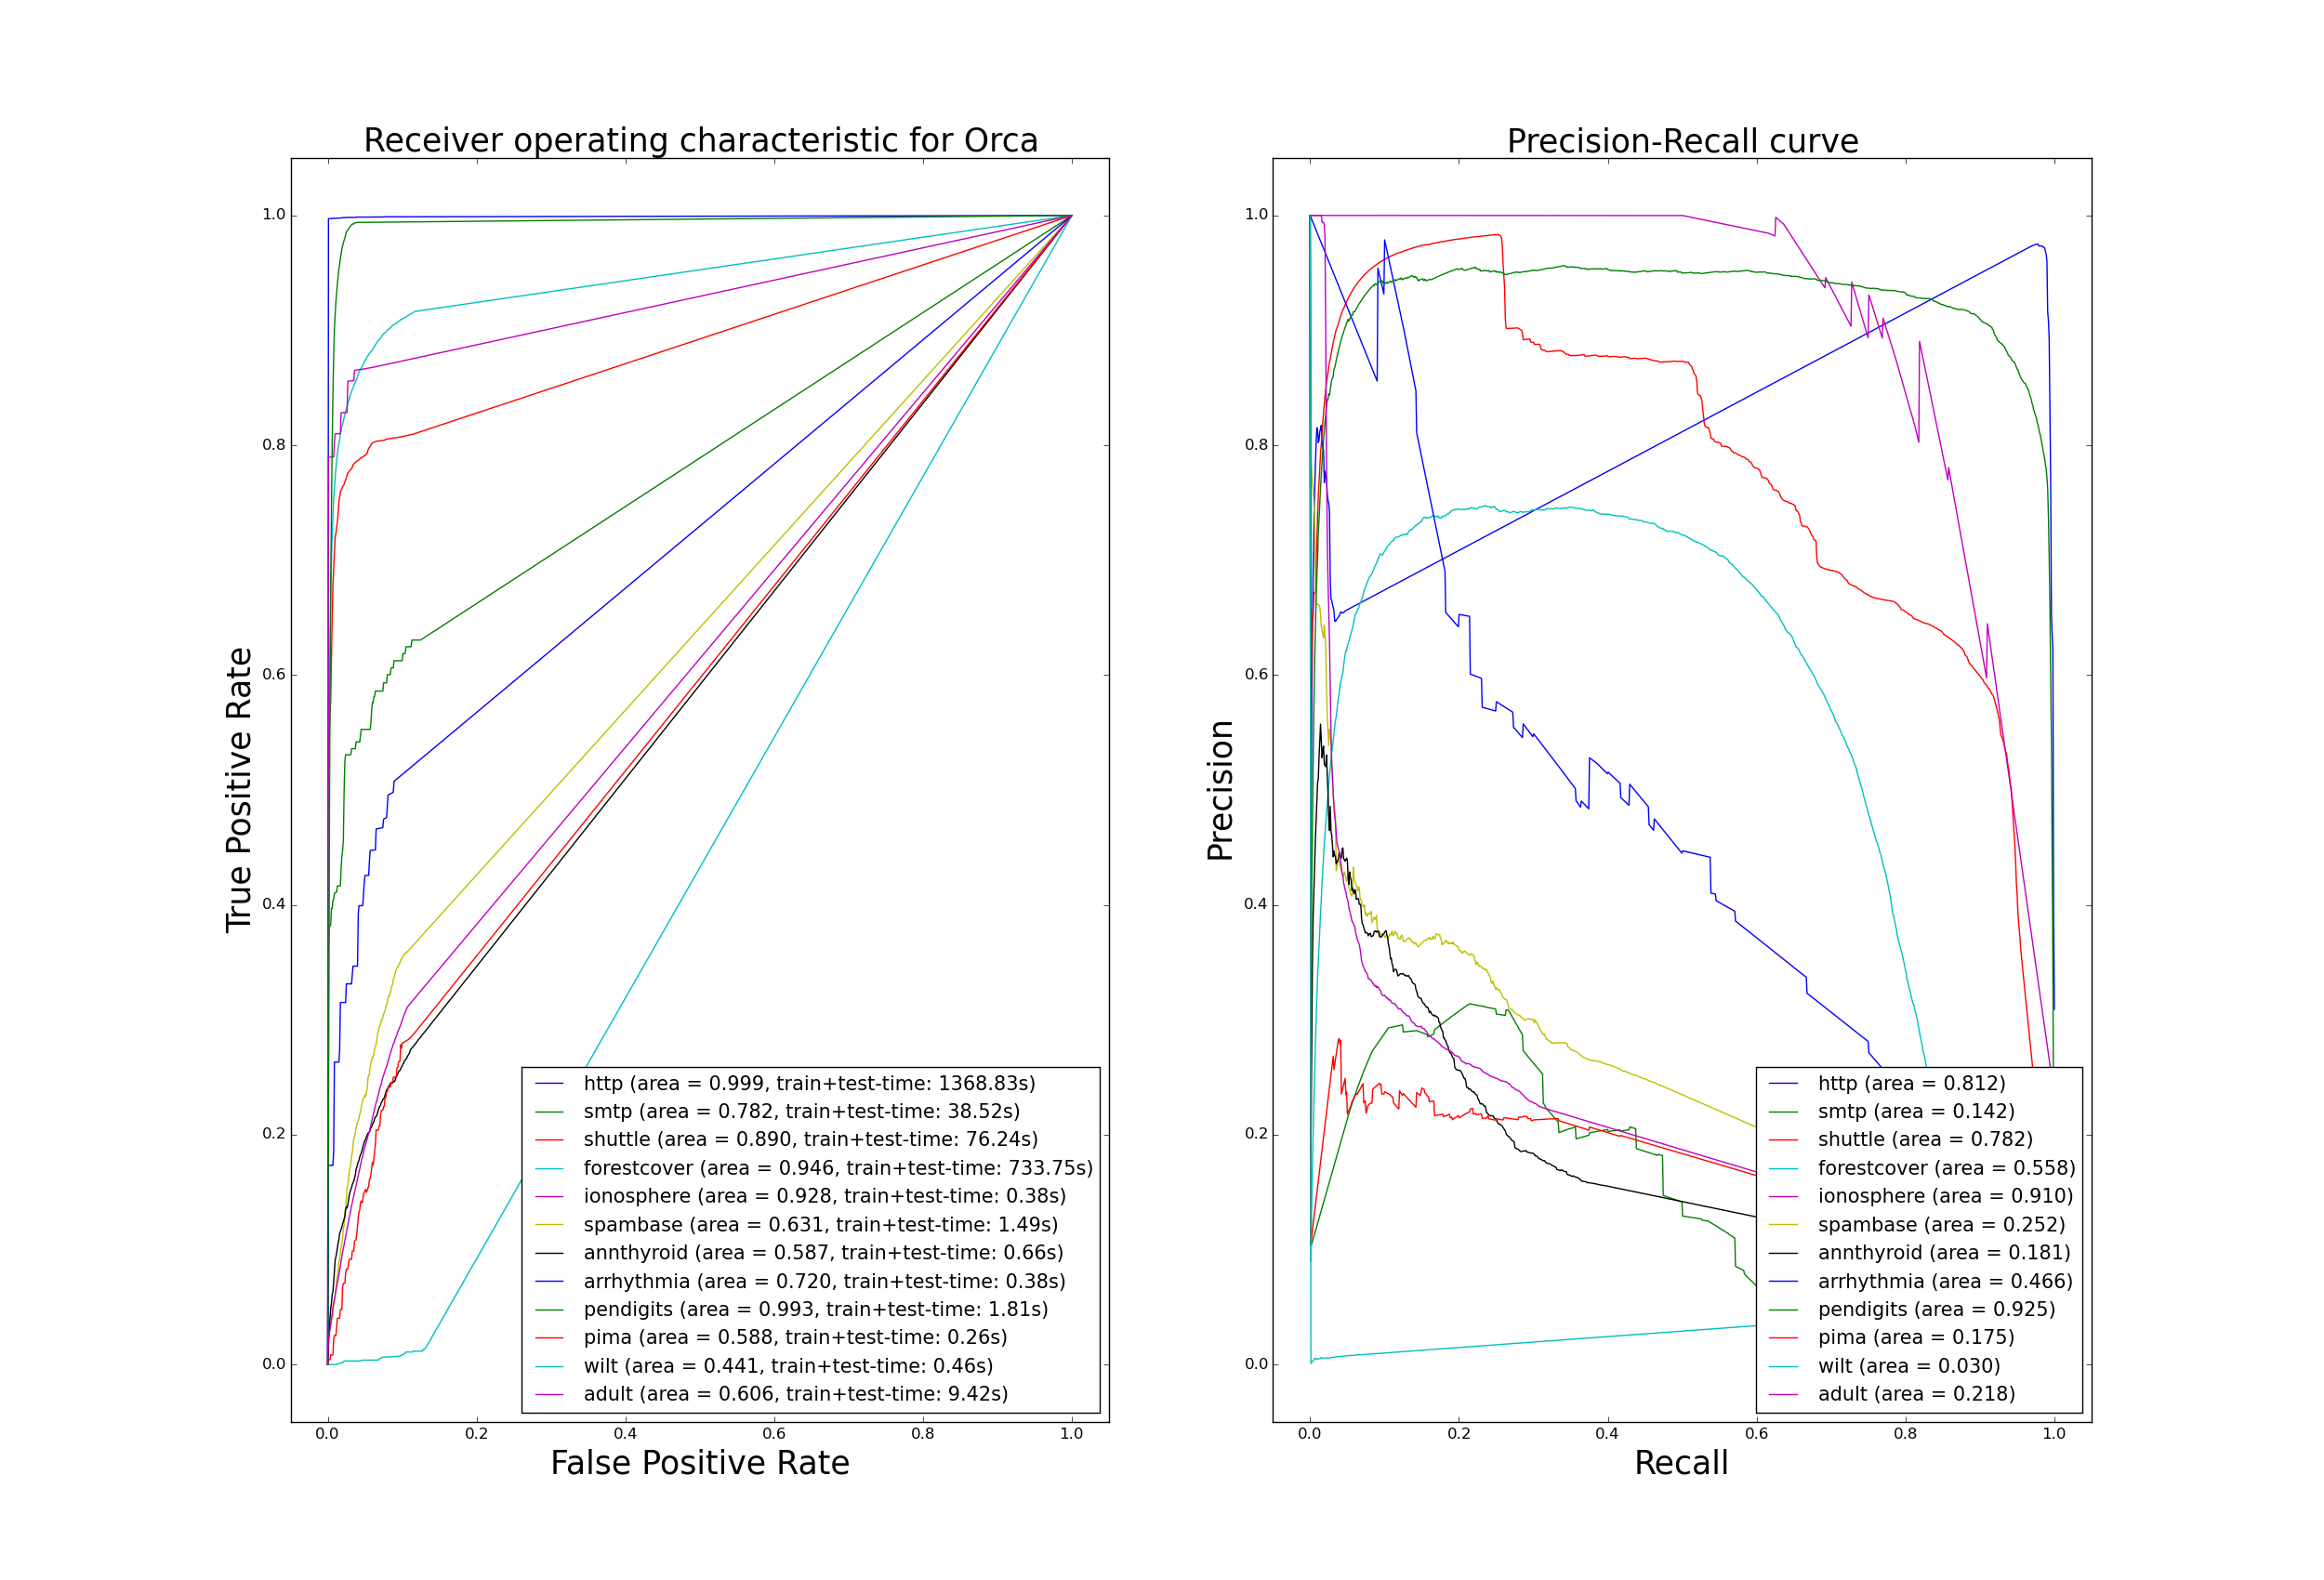
\includegraphics[trim=175 80 175 123, clip,
    width=0.75\textwidth]{./gfx/bench_orca_roc_pr_supervised_factorized.png}
\end{figure*}
\begin{figure*}[!ht]
    \caption{\acs{ROC} and \acs{PR} curves for Orca (outlier detection
    framework)}
    \label{ocrf:fig:orca_roc_pr_unsupervised}
    \centering
    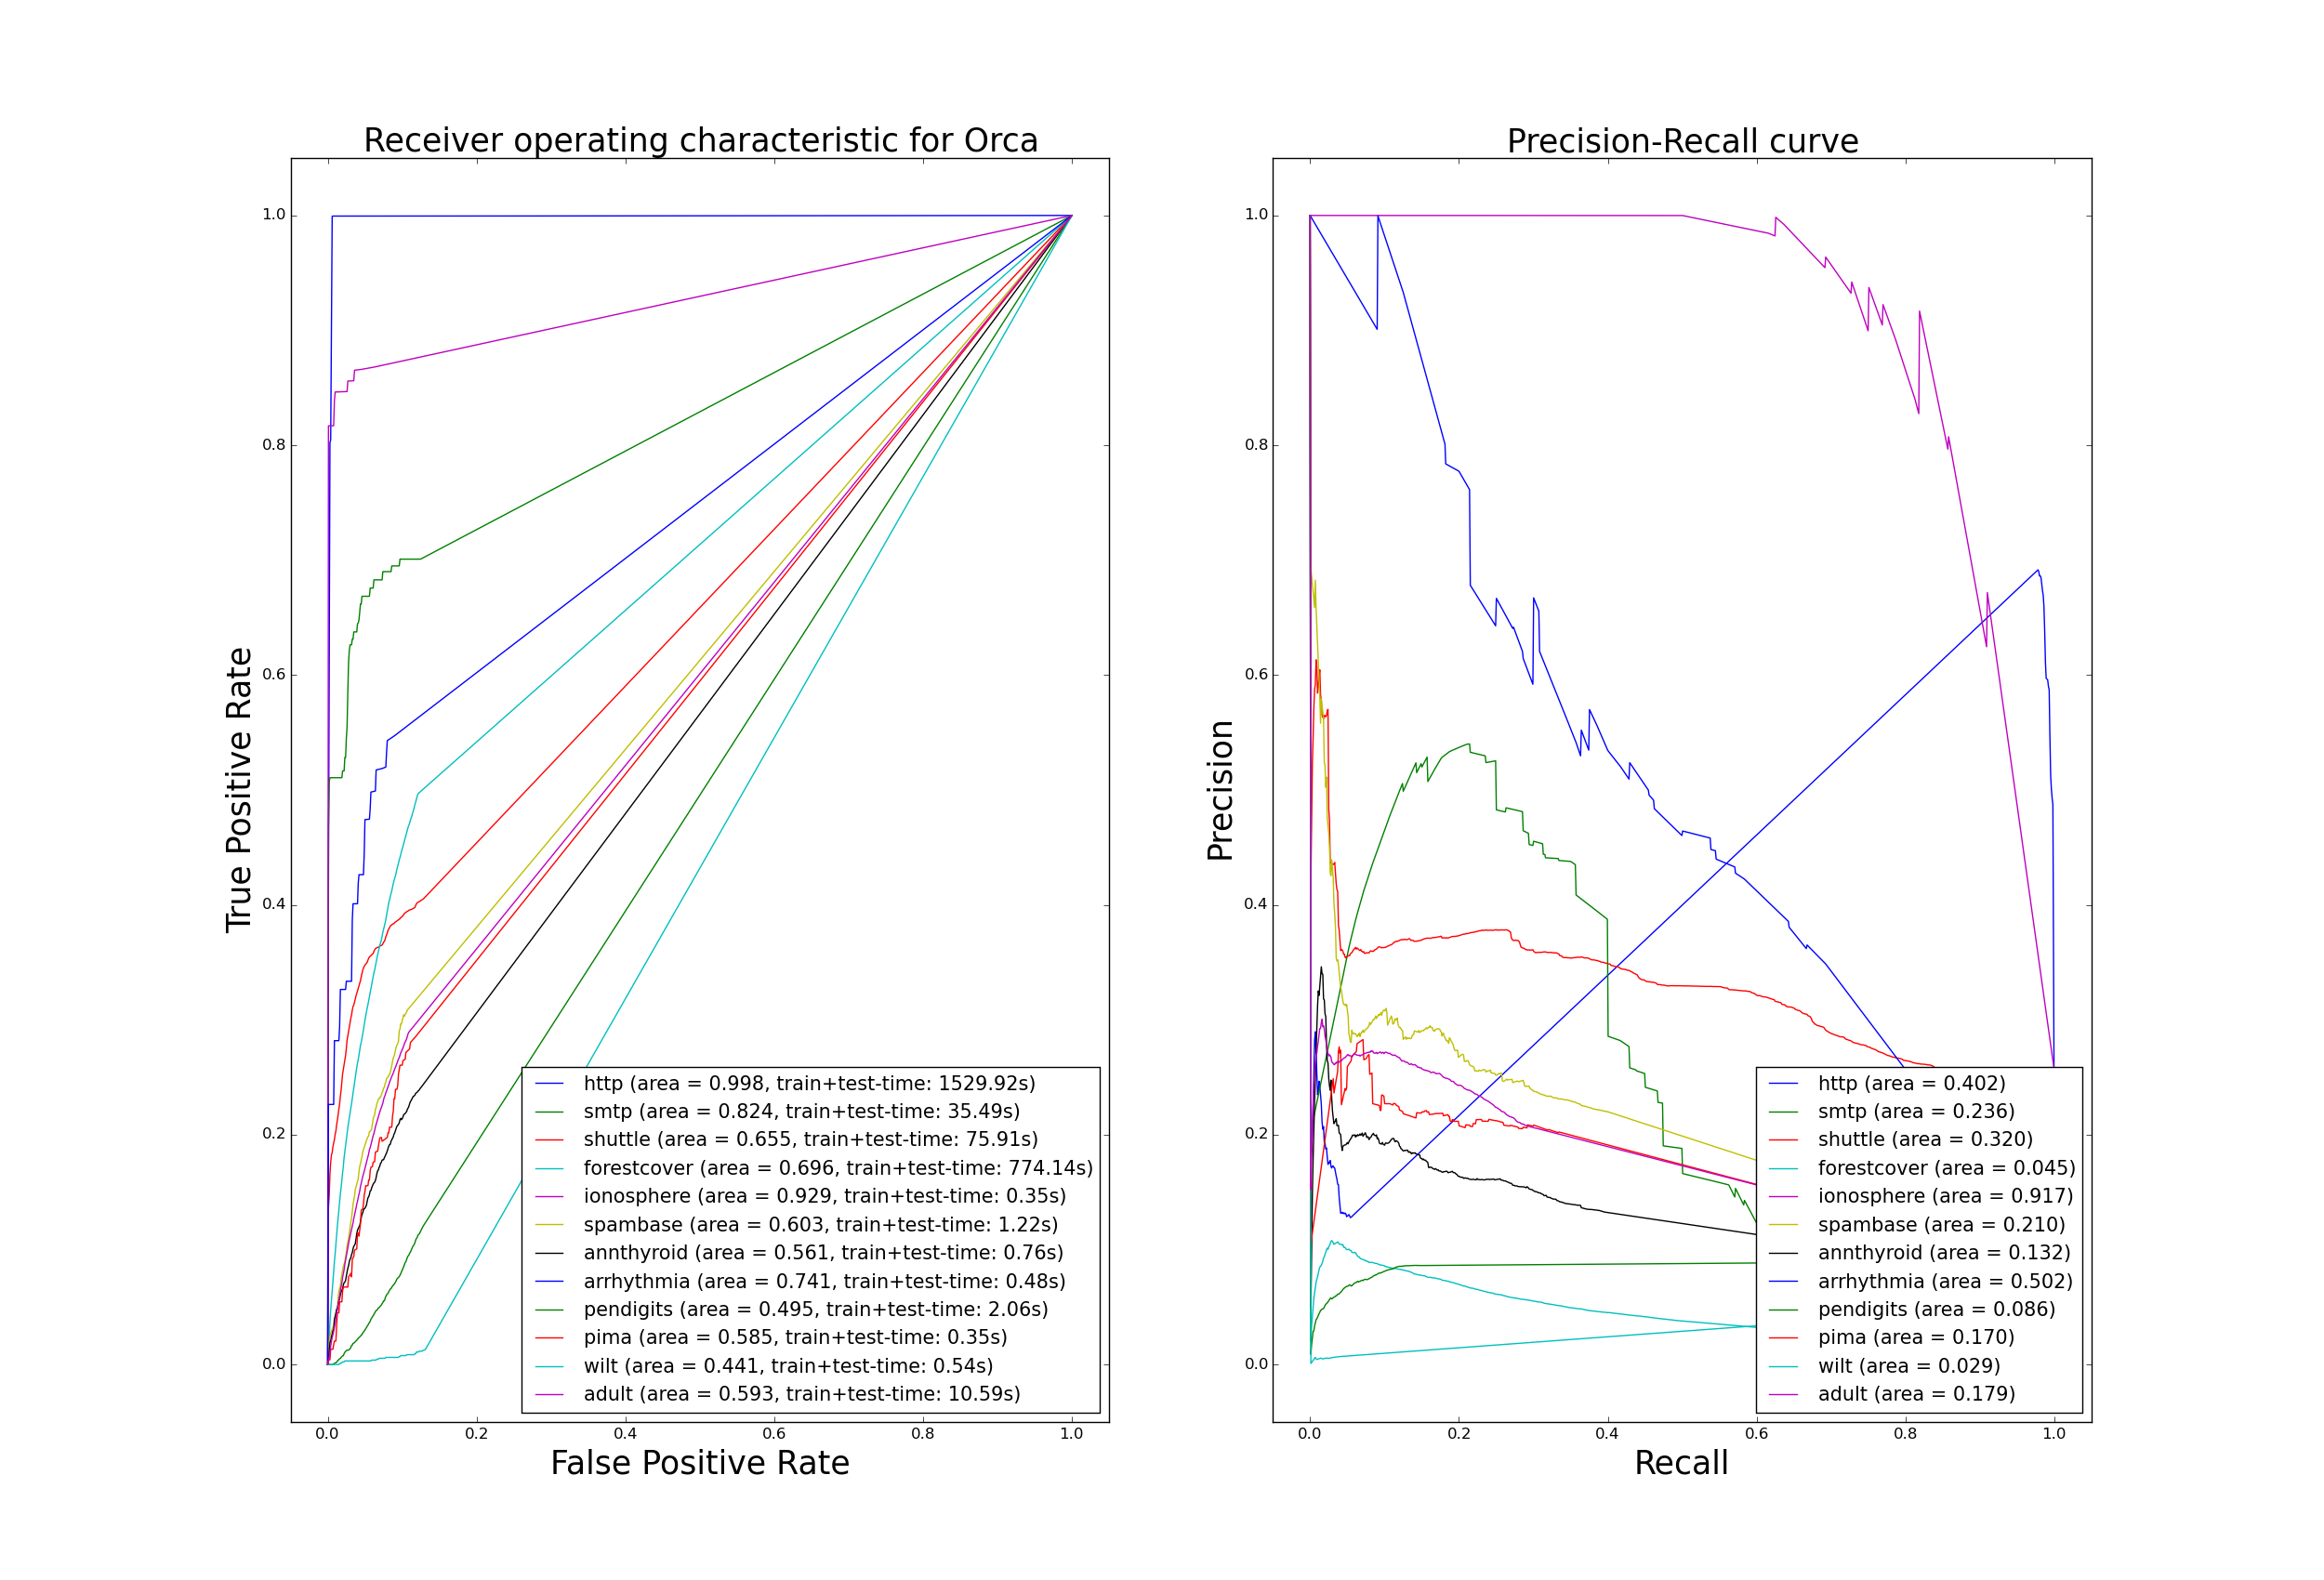
\includegraphics[trim=175 80 175 123, clip,
    width=0.75\textwidth]{./gfx/bench_orca_roc_pr_unsupervised_factorized.png}
\end{figure*}
\begin{figure*}[!ht]
    \caption{\acs{ROC} and \acs{PR} curves for \acs{LSAD} (novelty detection
    framework)}
    \label{ocrf:fig:LSAnomaly_roc_pr}
    \centering
    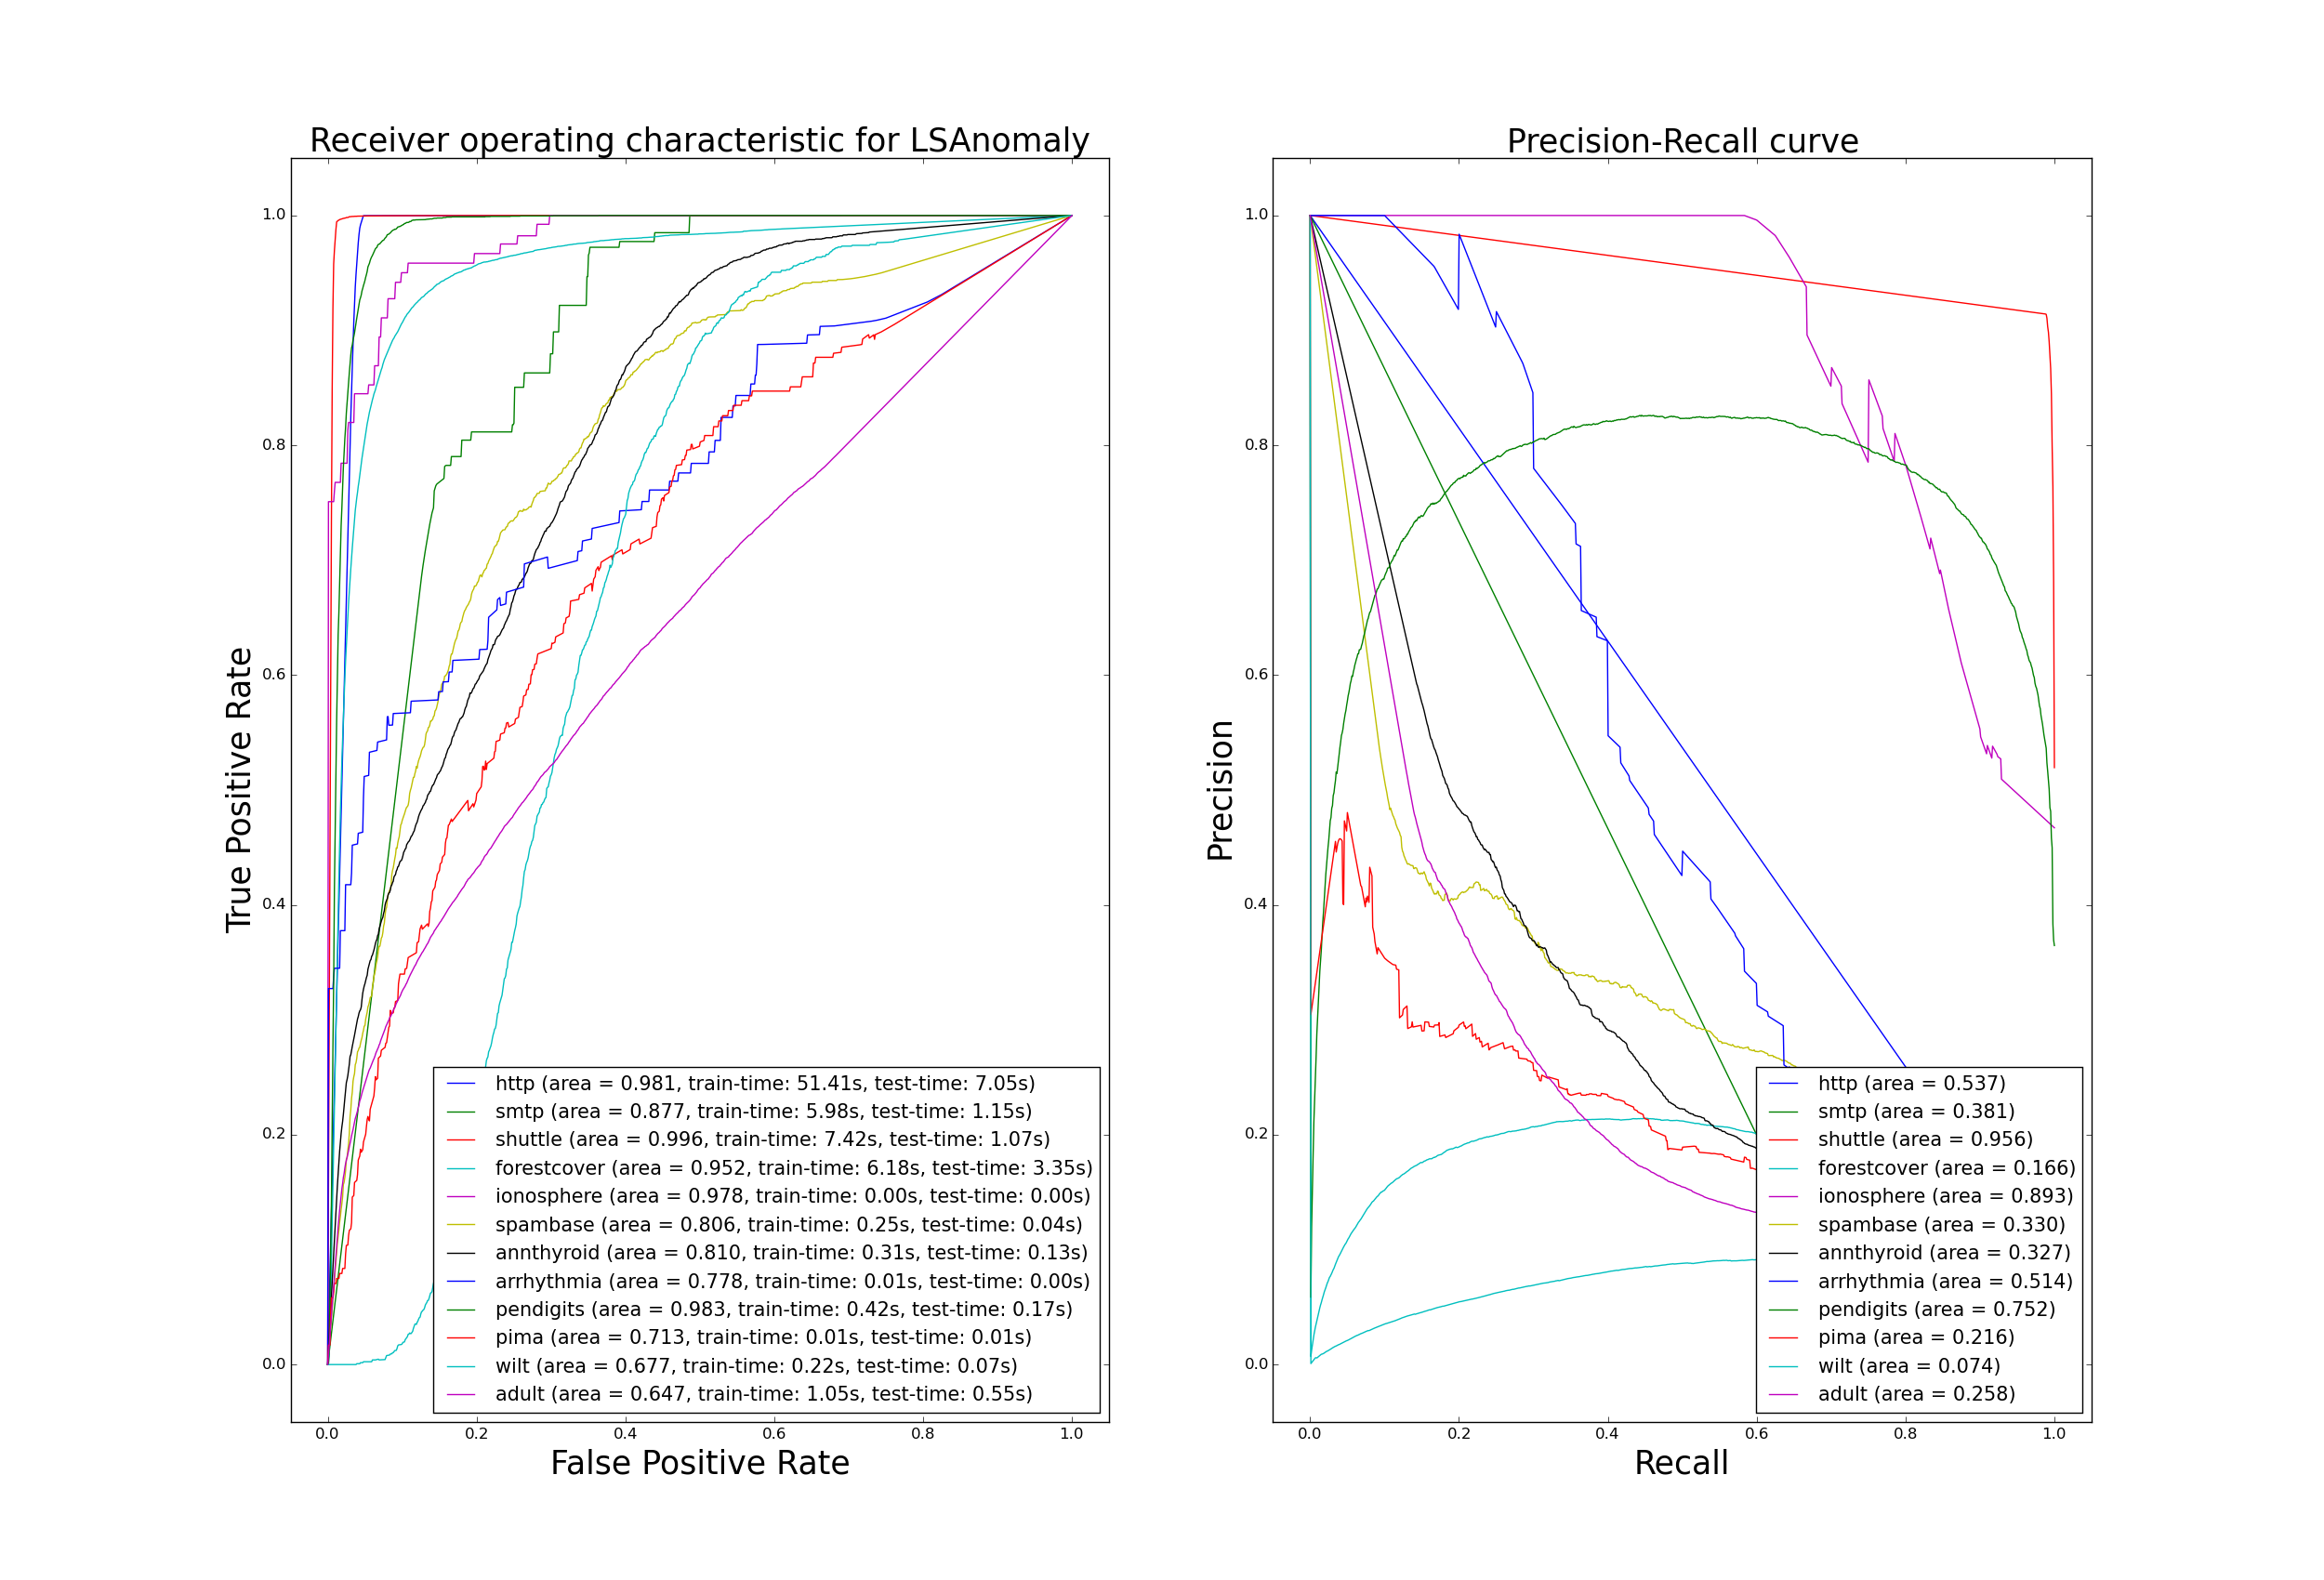
\includegraphics[trim=175 80 175 123, clip,
    width=0.75\textwidth]{./gfx/bench_LSAnomaly_roc_pr_supervised_factorized.png}
\end{figure*}
\begin{figure*}[!ht]
    \caption{\acs{ROC} and \acs{PR} curves for \acs{LSAD} (outlier detection
    framework)}
    \label{ocrf:fig:LSAnomaly_roc_pr_unsupervised}
    \centering
    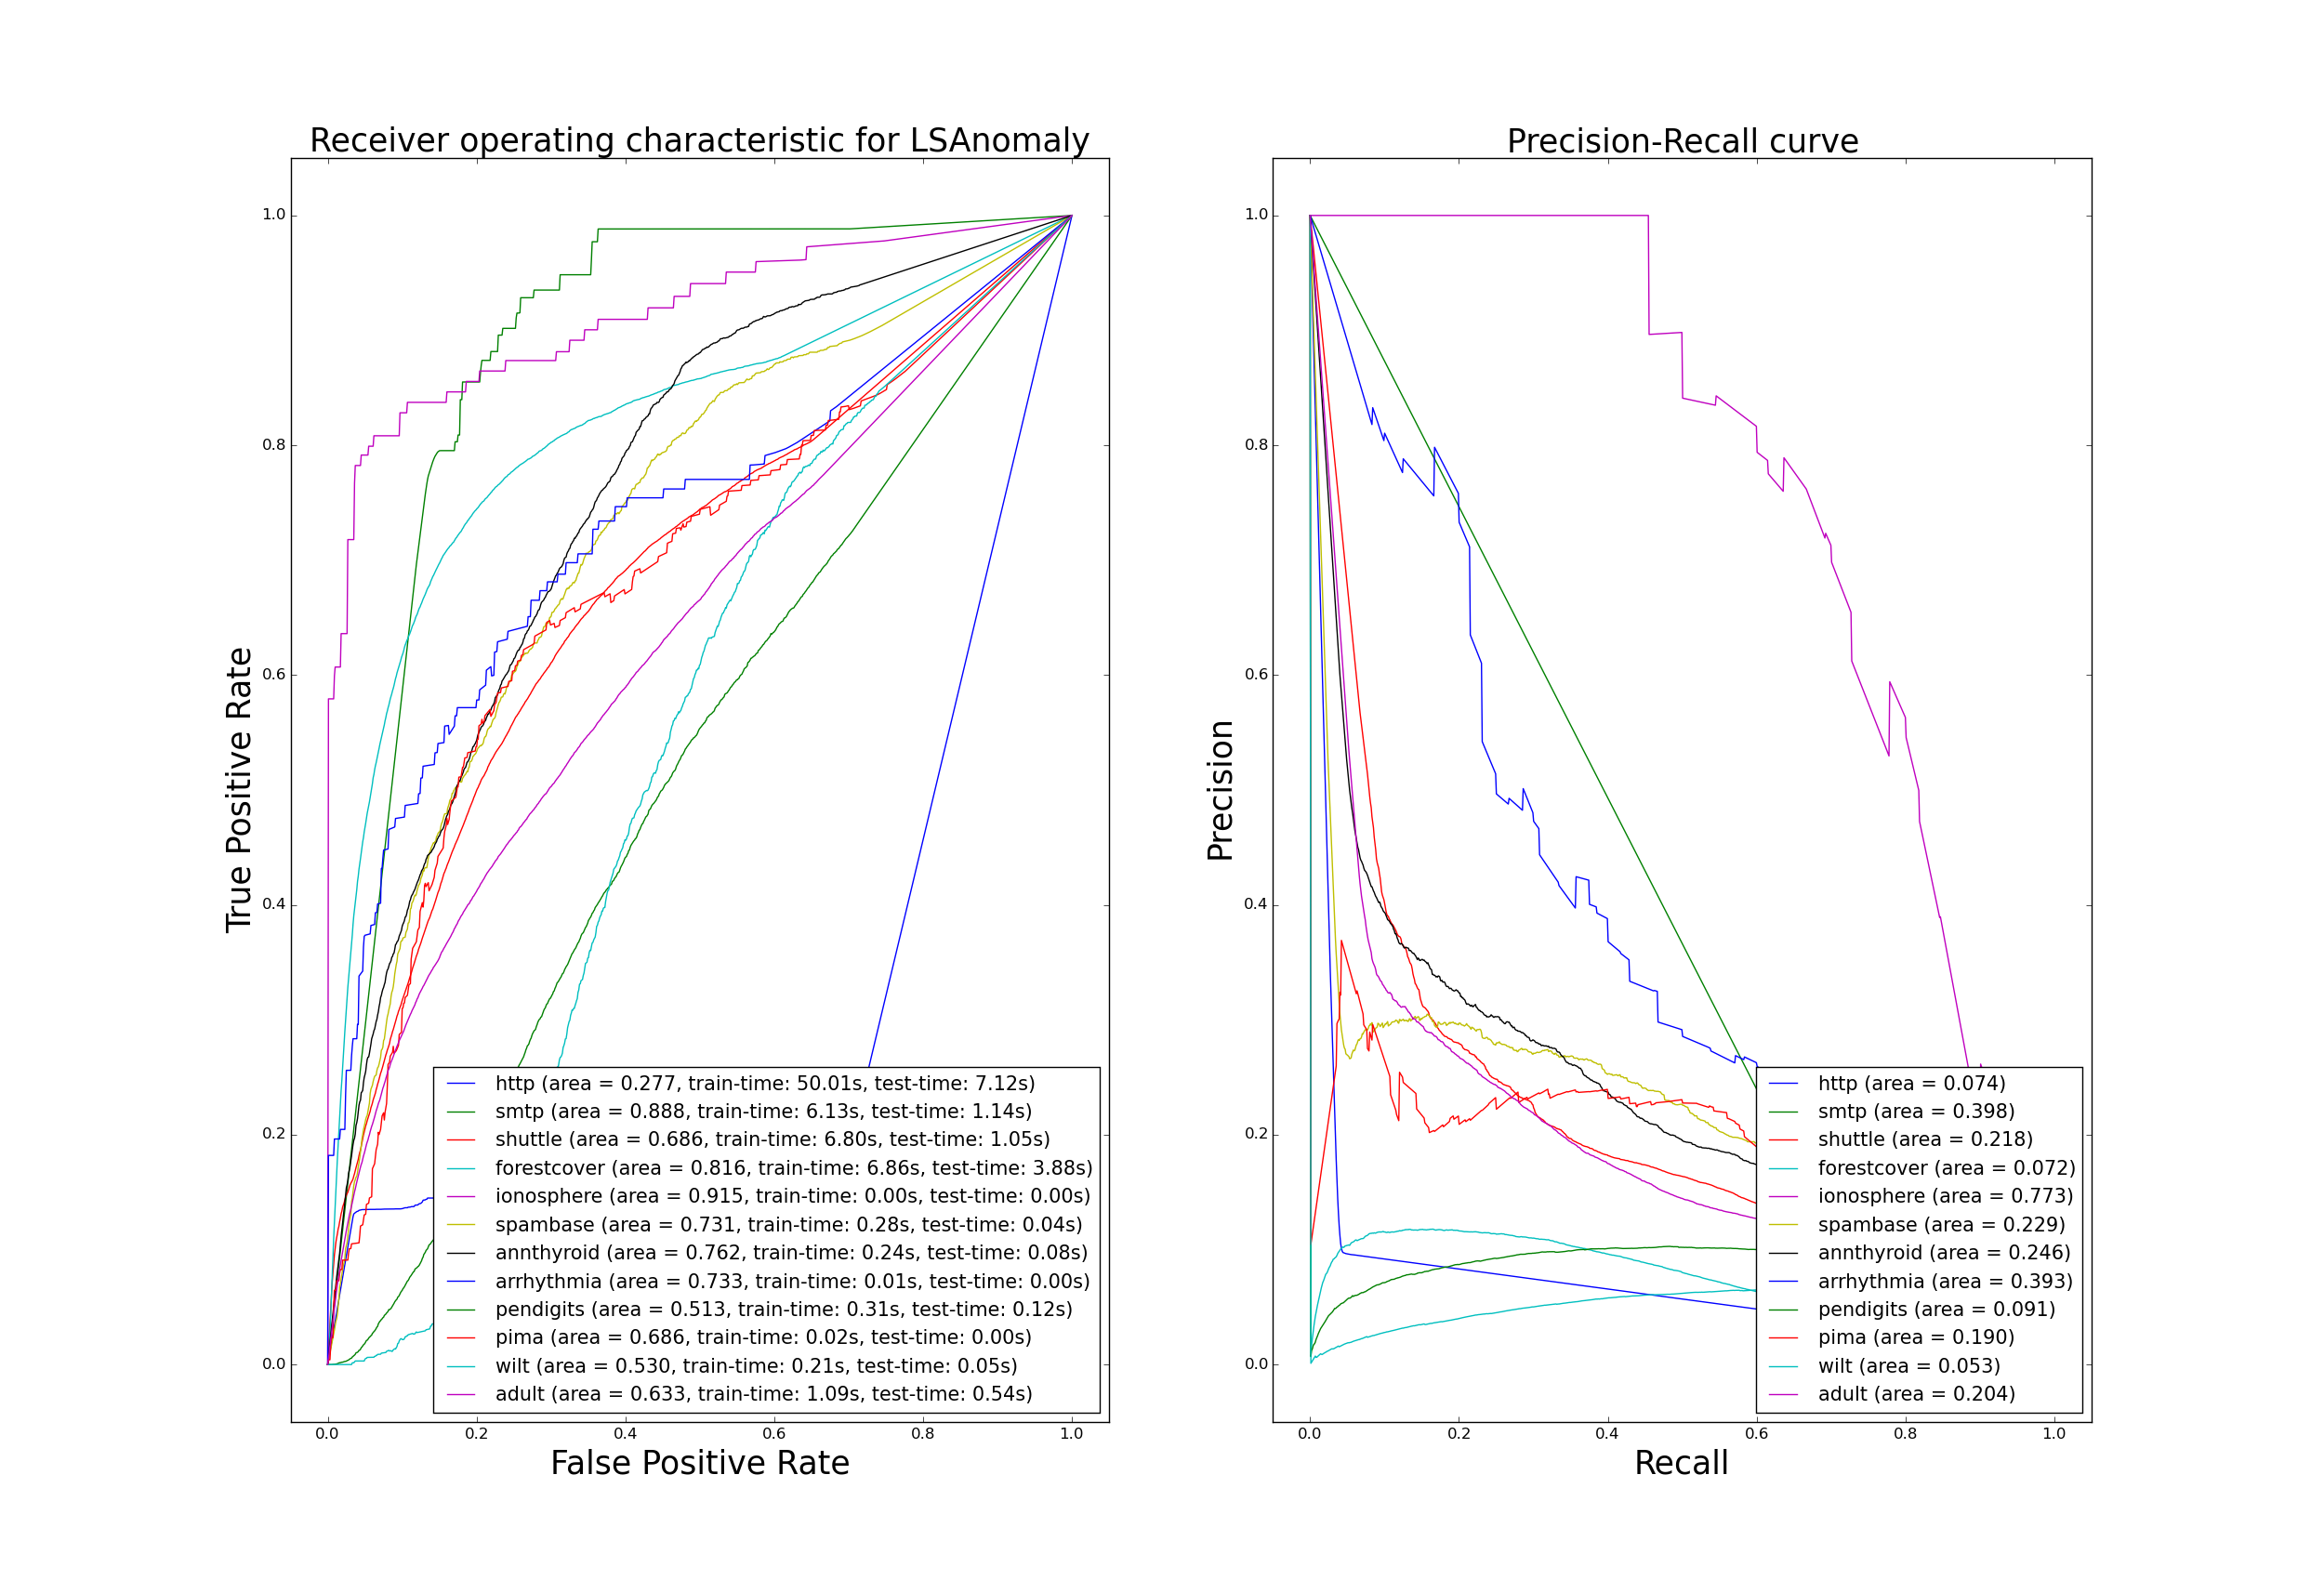
\includegraphics[trim=175 80 175 123, clip,
    width=0.75\textwidth]{./gfx/bench_LSAnomaly_roc_pr_unsupervised_factorized.png}
\end{figure*}
\begin{figure*}[!ht]
    \caption{\acs{ROC} and \acs{PR} curves for \acs{RFC} (novelty detection
    framework)}
    \label{ocrf:fig:rf_roc_pr}
    \centering
    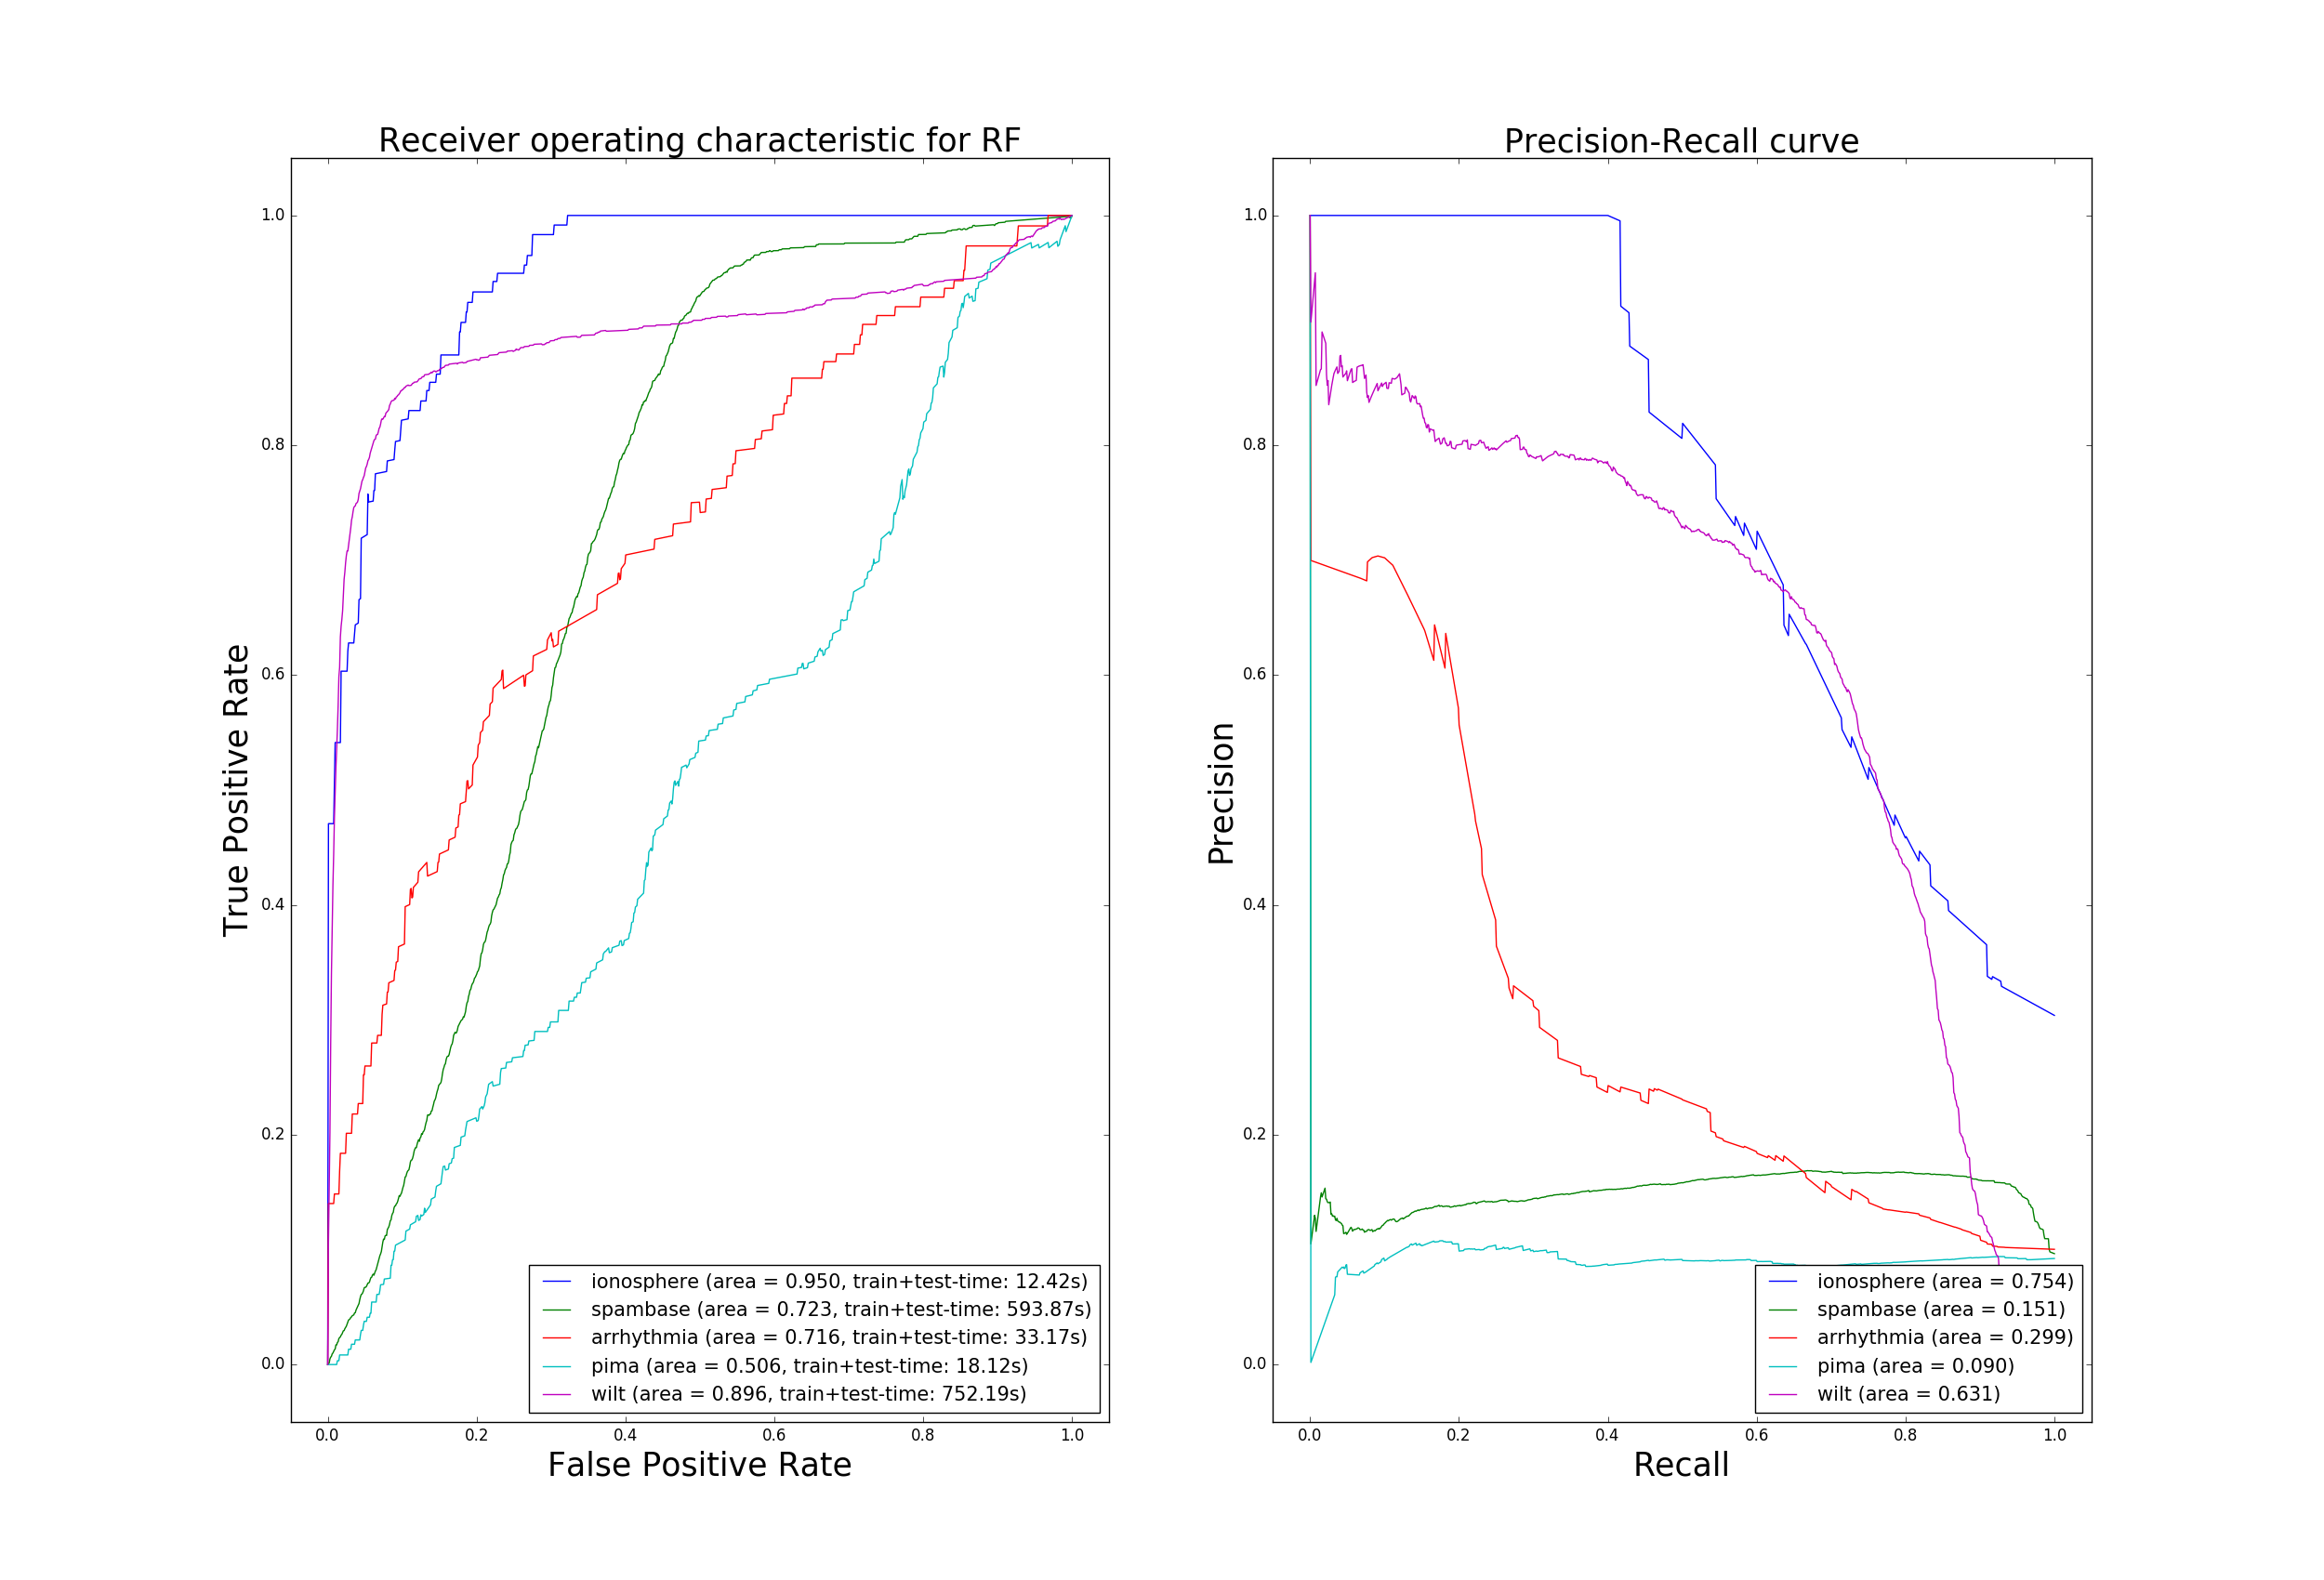
\includegraphics[trim=175 80 175 123, clip,
    width=0.75\textwidth]{./gfx/bench_rf_roc_pr_supervised_factorized.png}
\end{figure*}
\begin{figure*}[!ht]
    \caption{\acs{ROC} and \acs{PR} curves for \acs{RFC} (outlier detection
    framework)}
    \label{ocrf:fig:rf_roc_pr_unsupervised}
    \centering
    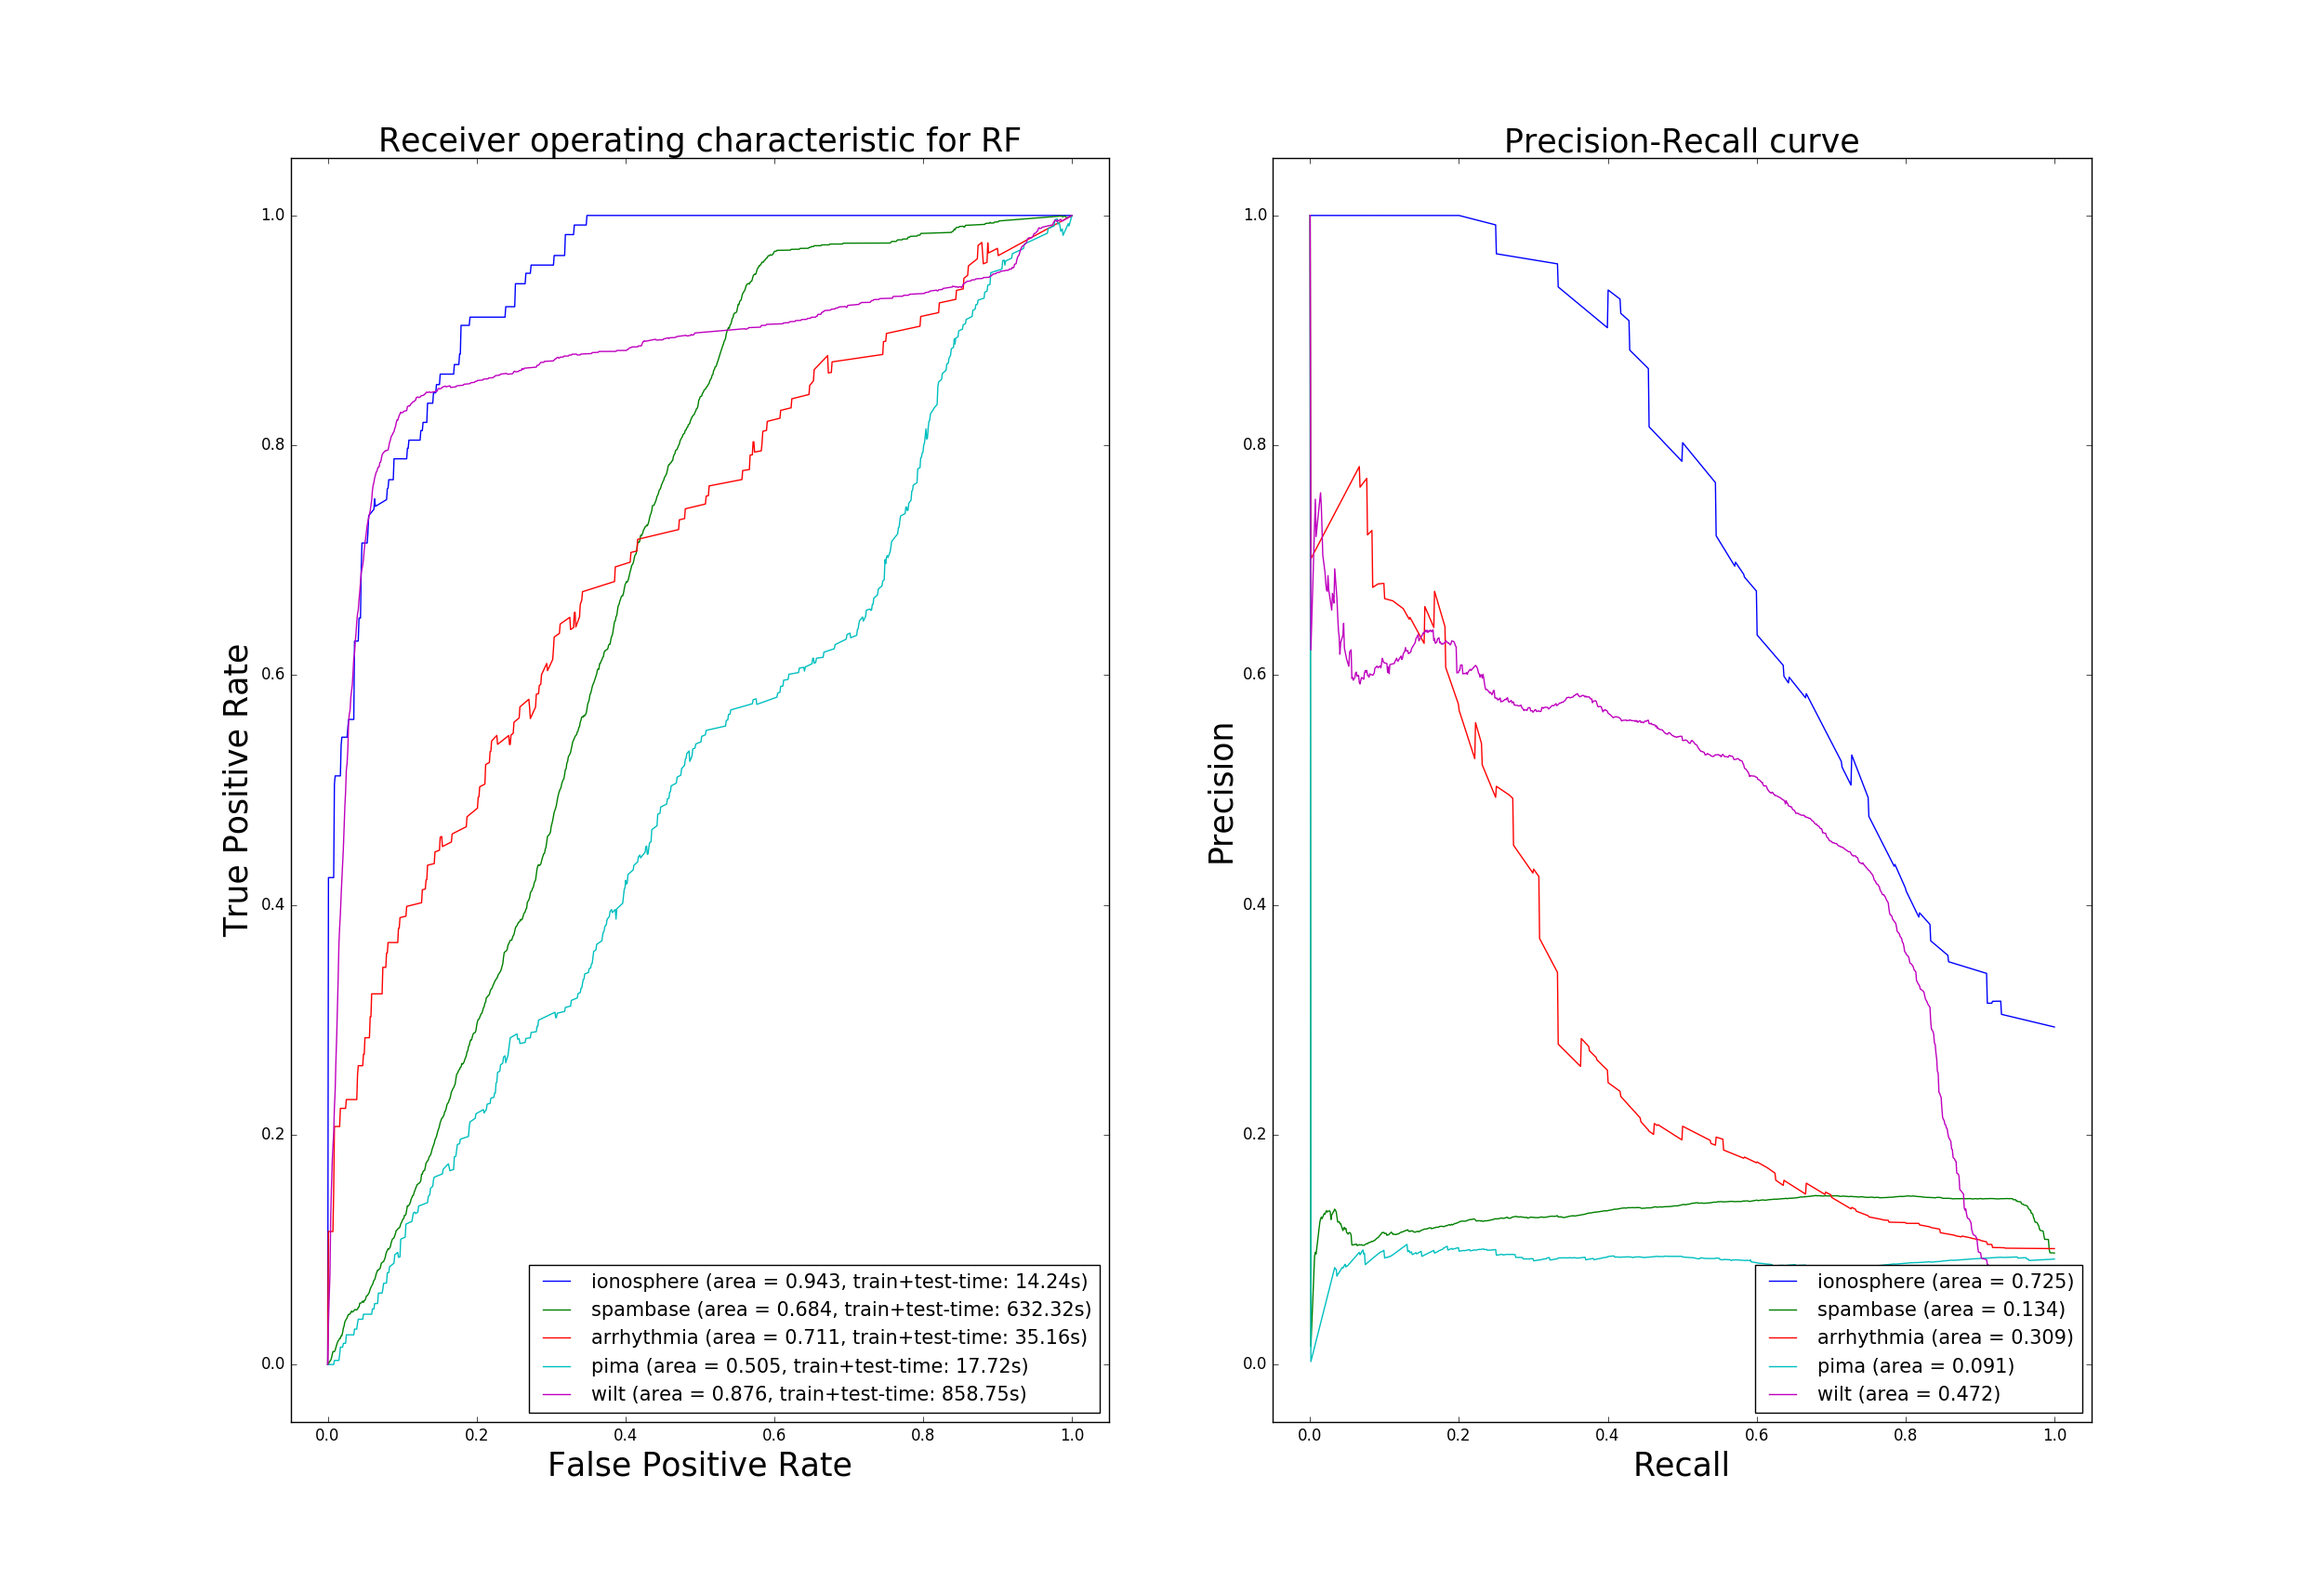
\includegraphics[trim=175 80 175 123, clip,
    width=0.75\textwidth]{./gfx/bench_rf_roc_pr_unsupervised_factorized.png}
\end{figure*}

%XXX TODO: description of the table
\afterpage{%
\begin{landscape}
    \begin{table}[htb]
        \caption{Results for the outlier detection setting}
        \label{ocrf:table:results-unsupervised}

        \centering
        %\scriptsize
        \resizebox{\textheight}{!}{%
        \begin{tabular}{lcccccccccccccccc}
        \toprule
            Dataset & \multicolumn{2}{c }{\acs{OneClassRF}} & \multicolumn{2}{c
            }{\acs{iForest}} & \multicolumn{2}{c }{\acs{OCRFsampling}} &
            \multicolumn{2}{c }{\acs{OCSVM}} & \multicolumn{2}{c }{\acs{LOF}} &
            \multicolumn{2}{c }{Orca}& \multicolumn{2}{c }{\acs{LSAD}}&
            \multicolumn{2}{c }{\acs{RFC}}  \\%&
            %parameters $(\epsilon, k)$\\
        \cmidrule{1-17}
            \acs{AUC}          & \acs{ROC} &  \acs{PR} & \acs{ROC} &  \acs{PR}
            & \acs{ROC} & \acs{PR}  & \acs{ROC} & \acs{PR}  & \acs{ROC} &
            \acs{PR} & \acs{ROC}  & \acs{PR}  & \acs{ROC} &  \acs{PR} &
            \acs{ROC} & \acs{PR}  \\
            adult                 & 0.625 & 0.161   & \textbf{0.644} & 0.234 &
            \acs{NA} & \acs{NA}     & 0.622 & 0.179   & 0.546 & 0.100   & 0.593
            & 0.179 & 0.633 & 0.204       & \acs{NA}   & \acs{NA}  \\
            annthyroid             & 0.842 & 0.226   & 0.820 & 0.310   &
            \textbf{0.992} & 0.869   & 0.688 & 0.193   & 0.731 & 0.188   &
            0.561 & 0.132   & 0.762 & 0.246       & \acs{NA}   & \acs{NA}  \\
            arrhythmia             & 0.698 & 0.485   & 0.746 & 0.418   & 0.704
            & 0.276   & \textbf{0.916} & 0.630   & 0.765 & 0.468   & 0.741 &
            0.502 & 0.733 & 0.393       & 0.711 & 0.309 \\
            forestcover             & 0.845 & 0.044   & \textbf{0.882} & 0.062
            & \acs{NA}  & \acs{NA}     & \acs{NA} & \acs{NA}   & 0.550 & 0.017
            & 0.696 & 0.045   & 0.816 & 0.072       & \acs{NA}   & \acs{NA} \\
            http                  & 0.984 & 0.120   & \textbf{0.999} & 0.685 &
            \acs{NA} & \acs{NA}    & \acs{NA} & \acs{NA}   & \acs{NA}   &
            \acs{NA}     & 0.998 & 0.402   & 0.277 & 0.074 & \acs{NA}   &
            \acs{NA}   \\
            ionosphere              & 0.903 & 0.508   & 0.888 & 0.545   & 0.879
            & 0.664   & \textbf{0.956} & 0.813   & \textbf{0.956} & 0.789   &
            0.929 & 0.917   & 0.915 & 0.773       & 0.943 & 0.725 \\
            pendigits             & 0.453 & 0.085   & 0.463 & 0.077   &
            \textbf{0.999} & 0.993   & 0.366 & 0.066   & 0.491 & 0.086   &
            0.495 & 0.086   & 0.513 & 0.091       & \acs{NA}   & \acs{NA}   \\
            pima & 0.708 & 0.229   & 0.743 & 0.205   & \textbf{0.790} & 0.296 &
            0.706 & 0.226   & 0.670 & 0.137   & 0.585 & 0.170   & 0.686 & 0.190
            & 0.505 & 0.091 \\
            shuttle               & 0.947 & 0.491   & \textbf{0.997} & 0.979 &
            \acs{NA} & \acs{NA}     & 0.992 & 0.904   & 0.526 & 0.115   & 0.655
            & 0.320 & 0.686 & 0.218       & \acs{NA}  & \acs{NA}   \\
            smtp                  & \textbf{0.916} & 0.400   & 0.902 & 0.005 &
            \acs{NA} & \acs{NA}     & 0.881 & 0.372   & 0.909 & 0.053   & 0.824
            & 0.236 & 0.888 & 0.398       & \acs{NA}   & \acs{NA}   \\
            spambase             & 0.830 & 0.300   & 0.799 & 0.303   &
            \textbf{0.970} & 0.877   & 0.722 & 0.192   & 0.664 & 0.120   &
            0.603 & 0.210   & 0.731 & 0.229       & 0.684 & 0.134 \\
            wilt                 & 0.520 & 0.053   & 0.443 & 0.044   &
            \textbf{0.966} & 0.554   & 0.316 & 0.036   & 0.627 & 0.069   &
            0.441 & 0.029   & 0.530 & 0.053       & 0.876 & 0.472 \\
            %internet_ads &     &       & & & & & & & &\\
        \cmidrule{1-17}
            average & 0.773 &  0.259 & 0.777 & 0.322 & \textbf{0.900} & 0.647 &
            0.717 & 0.361 & 0.676 & 0.195 & 0.677 & 0.269 & 0.681 & 0.245 &
            0.744 & 0.346 \\
            \acs{cum} train time & \multicolumn{2}{c }{\textbf{61s}} &
            \multicolumn{2}{c }{70s} & \multicolumn{2}{c }{\acs{NA}} &
            \multicolumn{2}{c }{\acs{NA}}& \multicolumn{2}{c }{\acs{NA}} &
            \multicolumn{2}{c }{2432s}& \multicolumn{2}{c }{72s}&
            \multicolumn{2}{c }{\acs{NA}}  \\
        \bottomrule
        \end{tabular}}
    \end{table}
\end{landscape}}
\FloatBarrier
\chapterend


